\documentclass[a4paper, 12pt]{amsart}
\usepackage{amssymb}
\usepackage{amsthm}
\usepackage{amsmath}
\usepackage{cite}
\usepackage{bbm}
\usepackage{stmaryrd} 
\usepackage{url} 
\usepackage{lineno}
\usepackage[margin=2.5cm]{geometry}
\usepackage{tikz}
\usetikzlibrary{arrows}
\usepackage{mathabx}



%Packages from forcing axiom paper
%\usepackage{aliascnt}
\usepackage[all,cmtip,color]{xy} 
\usepackage{float}
%\usepackage[dvipsnames]{xcolor}

\usepackage[textsize=footnotesize]{todonotes}
\newcommand{\comment}[1]{\todo[fancyline]{#1}}

%\pagenumbering{arabic}

%\setlength{\textwidth}{16cm}    %16
%\setlength\textheight{24.2cm}  %24.2
%\setlength\oddsidemargin{-0.2cm}
%\setlength\topmargin{-1cm}
%\setlength\footskip{-0.8cm}


%%%%%%% Hyperref setup
\usepackage{hyperref}
\definecolor{dblue}{rgb}{0,0,0.70}
\hypersetup{
	unicode=true,
	colorlinks=true,
	citecolor=dblue,
	linkcolor=dblue,
	anchorcolor=dblue, 
	urlcolor   = dblue
}


\newtheorem{lemma}{Lemma}[section]
\newtheorem*{lemma*}{Lemma}
\newtheorem{theorem}[lemma]{Theorem}
\newtheorem{corollary}[lemma]{Corollary}
\newtheorem{proposition}[lemma]{Proposition}
\newtheorem{claim}[lemma]{Claim}
\newtheorem*{subclaim}{Subclaim}
\newtheorem*{fact}{Fact}


%\newaliascnt{example}{theorem}
%\newtheorem{example}[example]{Example}
\newtheorem{example}{Example}
\newtheorem*{question*}{Question}

\theoremstyle{definition}
\newtheorem{definition}[lemma]{Definition}
\newtheorem*{definition*}{Definition}
\newtheorem*{notation}{Notation}
\newtheorem{question}{Question}

\newtheorem{remark}[lemma]{Remark}

%\usepackage{vmargin}
%\setpapersize{A4}
%\setmarginsrb{25mm}{10mm}{15mm}{10mm}{12pt}{11mm}{0pt}{11mm}

\DeclareMathOperator{\On}{On}
\DeclareMathOperator{\lub}{lub}
\DeclareMathOperator{\supp}{supp}
\DeclareMathOperator{\const}{const_0}
\DeclareMathOperator{\ran}{ran}
\DeclareMathOperator{\Lim}{Lim}
\DeclareMathOperator{\Card}{Card}
\DeclareMathOperator{\Reg}{Reg}
\DeclareMathOperator{\Def}{Def}
\DeclareMathOperator{\rud}{rud}
\DeclareMathOperator{\id}{id}
\DeclareMathOperator{\cf}{cf}
\DeclareMathOperator{\PFA}{\axiomft{PFA}}
\DeclareMathOperator{\Cof}{Cof}
\DeclareMathOperator{\Cofw}{Cof_\omega}
\DeclareMathOperator{\Omache}{O^{Machete_\epsilon}}
\DeclareMathOperator{\Omp}{O^{M\varphi}}
\DeclareMathOperator{\Ome}{O^{M\epsilon}}
\DeclareMathOperator{\Omn}{O^{Mn}}
\DeclareMathOperator{\Omepsilon}{O^{M\epsilon}}
\DeclareMathOperator{\Oml}{O^{M\lambda}}
\DeclareMathOperator{\dom}{dom}
\DeclareMathOperator{\Ult}{Ult}
\DeclareMathOperator{\ZFC}{\axiomft{ZFC}}
\DeclareMathOperator{\ZF}{\axiomft{ZF}}
\DeclareMathOperator{\MK}{MK}
\DeclareMathOperator{\LST}{LST}
\DeclareMathOperator{\NM}{NM}
\DeclareMathOperator{\col}{Col}
\DeclareMathOperator{\height}{ht}
\DeclareMathOperator{\length}{length}

\newcommand{\PP}{\mathbb{P}}
\newcommand{\QQ}{\mathbb{Q}}
\newcommand{\RR}{\mathbb{R}}
\newcommand{\BB}{\mathbb{B}}

%Commands for the forcing axiom paper
\newcommand{\axiomft}[1]{\mathsf{#1}} 
\newcommand{\FA}{\mathsf{FA}}
\newcommand{\BFA}{\mathsf{BFA}}
\newcommand{\NP}{\mathsf{N}}
\newcommand{\BN}{\mathsf{BN}}
%{\mathsf{NP}}
\newcommand{\club}{\mathsf{club}\text{-}}
\newcommand{\stat}{\mathsf{stat}\text{-}}
\newcommand{\ub}{\mathsf{ub}\text{-}}
\newcommand{\spec}{\mathrm{spec}}
\newcommand{\rspec}{\mathrm{rspec}}
\newcommand{\bspec}{\mathrm{bspec}}
\newcommand{\brspec}{\mathrm{brspec}}
\newcommand{\fo}{\Sigma_0^{\mathrm{(sim)}}\text{-}}
\newcommand{\bfo}{\mathrm{bsim}}
\newcommand{\sforces}{\Vdash^+} 
%{\Vvdash}
\newcommand{\Tr}{\mathrm{Tr}}
\newcommand{\forces}{\mathrel{\Vdash}}
\newcommand{\MA}{\axiomft{MA}}
\newcommand{\CH}{\axiomft{CH}}
\DeclareMathOperator{\crit}{crit}
\newcommand{\cof}{\mathrm{Cof}}
\newcommand{\Lev}{\mathrm{Lev}}
\newcommand{\pow}{\mathcal{P}}
\DeclareMathOperator{\rank}{rank}
\DeclareMathOperator{\Add}{Add}

\DeclareMathOperator{\Meas}{Meas}
\DeclareMathOperator{\Core}{Core}
\DeclareMathOperator{\Succ}{Succ}

\DeclareMathOperator{\form}{Form}

\newcommand{\bbfamily}{\fontencoding{U}\fontfamily{bbold}\selectfont}
\DeclareMathAlphabet{\mathbbold}{U}{bbold}{m}{n}


\usepackage{enumitem}

\newenvironment{enumerate-(a)}{\begin{enumerate}[label={\upshape (\alph*)}, leftmargin=2pc]}{\end{enumerate}}
\newenvironment{enumerate-(1)}{\begin{enumerate}[label={\upshape (\arabic*)}, leftmargin=2pc]}{\end{enumerate}}
\newenvironment{enumerate-(i)}{\begin{enumerate}[label={\upshape (\roman*)}, leftmargin=2pc]}{\end{enumerate}}
\newenvironment{itemizenew}{\begin{itemize}[leftmargin=2pc]}{\end{itemize}}

\title{LST Numbers for $Q^\text{e.c.}$ and $I$ style quantifiers}
\author{Christopher Turner}
\address{School of Mathematics, 
	University of Bristol, 
	Fry Building.
	Woodland Road, 
	Bristol, BS8~1UG, UK}
\email{christopher.turner@bristol.ac.uk}

\date{\today}
\keywords{L\"owenheim-Skolem-Tarski numbers, H\"artig quantifier, equal cofinality quantifier}

\thanks{This paper is adapted from part of the author's Ph.D. thesis, and he is grateful to his supervisor Philip Welch for his invaluable guidance. He would also like to thank Andrew Brooke-Taylor and Jonathan Osinski for pointing out various glitches in a previous version of the paper. The author was supported in his research by EPSRC grant EP/R513179/1 and a scholarship from the Heilbronn Institute, and by an internal grant from the University of Bristol. For the purpose of open access, the author has applied a ‘Creative Commons Attribution' (CC BY) public copyright licence to any Author Accepted Manuscript (AAM) version arising from this submission.} 

\begin{document}
	
	\begin{abstract}
		We introduce two schemes of quantifiers analogous to $I$ and $Q^\text{e.c.}$, which tell us about regular cardinals of small Cantor-Bendixson rank. We examine how the L\"owenheim-Skolem-Tarski numbers of these quantifiers interact with one another, and with those of $I$ and $Q^{\text{e.c.}}$. We then find the exact lower bound for each of the $\LST$ numbers, assuming the consistency of supercompacts.
	\end{abstract}
	
\maketitle
	
\section{Introduction}

%\todo[inline]{Work through the proof, getting rid of bits that give too much detail

%Ask Philipp if he can cite that lemma - see todonote.}

The L\"owenheim-Skolem theorem famously says that for any first-order language $\mathcal{L}$, any first order $\mathcal{L}$ structure contains an elementary substructure of size less than $\max(\lvert \mathcal{L}\rvert,\omega_1)$. The concept of the L\"owenheim-Skolem-Tarski number generalises this to simple second order logics. The $\LST$ number of a second-order logic is the smallest cardinal $\kappa$ such that every structure contains a substructure of size less than $\kappa$.

In \cite{magidorVaananan}, Magidor and V\"a\"an\"anen investigate $\LST$ numbers for two second order quantifiers: the H\"artig quantifier $I$ and the equal cofinality quantifier $Q^{\text{e.c.}}$. Roughly speaking, we can think of $I$ as telling us about the class $\Card$ of all cardinals (or, equivalently, about the class of all successor cardinals), while $Q^{\text{e.c.}}$ tells us about the class $\Reg$ of all (infinite) regular cardinals. In both cases, the lower bound turns out to be precisely the smallest sort of large cardinal which is not identified by the quantifier:

\begin{theorem}[Magidor,V\"a\"an\"anen]\cite[7, 20 \& 21]{magidorVaananan}
	If it exists, then $\LST(I)$ is at least the first inaccessible cardinal. Similarly, $\LST(I,Q^{\text{e.c.}})$ is at least the first Mahlo cardinal, if it exists. Moreover, if it is consistent that a supercompact cardinal exists then it is also consistent that either one of these $\LST$ numbers is exactly equal to the bound given.
\end{theorem}

In this paper, we introduce a suite of new intermediate results, establishing that this rule -- that the lower bound of $\LST(Q)$ is the least cardinal not identified by a quantifier $Q$ -- is true more generally in this region. Specifically, we shall look at quantifiers which tell us about simple fragments of $\Reg$ in ways similar to how $I$ tells us about $\Card$ and $Q^{\text{e.c.}}$ tells us about $\Reg$.

The fragments of $\Reg$ we are interested in are those of low \textit{Cantor-Bendixson} rank:

\begin{definition}
	For $\alpha\in \On$, we recursively define the classes $\Reg_\alpha$, $\Reg_{\geq \alpha}$ and $\Reg_{<\alpha}$ as follows:
	\begin{itemize}
	\item $\Reg_{<\alpha}:= \bigcup_{\beta<\alpha} \Reg_\beta$
	\item $\Reg_{\geq \alpha}=\Reg\setminus \Reg_{<\alpha}$
	\item $\Reg_\alpha$ is the class of successors of the club generated by $\Reg_{\geq\alpha}$
\end{itemize}
\end{definition}

So $\Reg_0$ is the class of successor cardinals, $\Reg_1$ is the class of simple inaccessibles, and so on.

The Cantor-Bendixson hierarchy is the natural partition to use if we're looking for something intermediate between $\Card$ and $\Reg$. The class $\Card$ is simply $\Reg_0$ together with its class of limits, and thus $\Card$ and $\Reg_0$ are mutually definable. Meanwhile the class ${\Reg_{<\infty}:=\bigcup_{\alpha\in \On}\Reg_{<\alpha}}$ is mutually definable with $\Reg$. (It's not \textit{quite} the same as $\Reg$, because $\omega$ is not in any $\Reg_\alpha$. But of course, we can easily handle this by defining $\omega$ directly.) And each individual class $\Reg_\alpha$ looks a lot like $\Reg_0$, the class defining $\Card$ -- for any $\alpha$, $\Reg_\alpha$ is a discrete sequence of $V$-cardinals.

We will introduce two new natural classes of quantifiers, $Q^\alpha$ and $R^\alpha$ (for arbitrary $\alpha$), which each tell us about $\Reg_{<\alpha}$. We will give an account of how the $\LST$ numbers of these quantifiers relate to one another, showing they are closely linked with each other and with $I$ and $Q^{\text{e.c.}}$. We will then show that $\min (\Reg_\alpha)$ is a lower bound for both $\LST(I,Q^\alpha)$ and $\LST(I,R^\alpha)$, and show that -- assuming the consistency of supercompacts -- there exist universes in which the $\LST$ numbers are both equal to this lower bound.

\section{Preliminaries}

We shall begin with some brief clarificatory definitions of the standard concepts we referred to in the introduction.

\begin{definition}
	
	A quantifier is a formal symbol $Q$, which is equipped with an arity $n\in \omega$ and a number $m\in \omega$, called the number of variables it quantifies over.
\end{definition}

\begin{definition}
	Let $\mathcal{L}$ be a first order language, and let $Q$ be an $n$-ary quantifier over $m$ variables. The language $\mathcal{L}\cup \{Q\}$ consists of the following formulas:
	\begin{itemize}
		\item Atomic formulas of $\mathcal{L}$
		\item $\neg \varphi$ and $\varphi \implies \psi$, whenever $\varphi$ and $\psi$ are formulas
		\item $\forall v (\varphi)$ where $v$ is any variable and $\varphi$ is a formula
		\item $Q v_1,\ldots,v_m (\varphi_1,\ldots,\varphi_n)$ where $v_1,\ldots,v_m$ are any variables (not necessarily distinct) and $\varphi_1,\ldots,\varphi_n$ are formulas
	\end{itemize}

	If $Q_1,\ldots,Q_k$ are quantifiers then $\mathcal{L} \cup \{Q_1,\ldots,Q_n\}$ is defined similarly.
\end{definition}

We are specifically interested in quantifiers like $\forall$, which have a single canonical interpretation.

\begin{definition}
%	A \textit{predefined} quantifier is a pair $(Q, \mathcal{I})$, where $Q$ is an $n$-ary quantifier in $m$ variables, and $\mathcal{I}$ encodes, for any set $A$, a subset $Q^A$ of functions from $A^m$ to $\{T,F\}^n$. If $\mathcal{I}$ is obvious, we will omit it.
	A \textit{predefined} quantifier is an $n$-ary quantifier symbol $Q$ in $m$ variables (for some $n$ and $m$), together with a fixed rule on how to interpret $Q v_1,\ldots,v_m (\varphi_1,\ldots,\varphi_n)$, for any second-order formulas $\varphi_1,\ldots,\varphi_n$ in \textit{any} language $\mathcal{L}$ including $Q$, over any $\mathcal{L}$ structure $\mathcal{A}$ and assignment of variable symbols to elements of $\mathcal{A}$. Usually, this guideline will be expressed in a recursive manner, with the interpretation of $Q v_1,\ldots,v_m (\varphi_1,\ldots,\varphi_n)$ dependent on the interpretations of $\varphi_1,\ldots,\varphi_n$.
\end{definition}

The details of how we formalise this concept are left to the reader: there are several different options.

A trivial example might make the idea here clearer.

\begin{example}
	$\forall$ is a predefined $1$-ary quantifier, which quantifies over one variable. $\forall v_1 \varphi$ is true (for a given $\varphi=\varphi(v_1)$, $\mathcal{A}$ and assignment) if and only if for all $x\in \mathcal{A}$, $\varphi(x)$ is interpreted as true. Similarly, $\exists$ is also a predefined $1$-ary quantifier, which again quantifies over one variable. 
\end{example}

The two well-known quantifiers mentioned in the introduction also have this predefined property.

\begin{definition}
	The H\"artig quantifier $I$ is $2$-ary, and quantifies over two variables. $I v_1,v_2 (\varphi,\psi)$ is interpreted as true (in a structure $\mathcal{A}$ over which we can interpret $\varphi$ and $\psi$, and have defined an assignment for variable symbols) if and only if the two sets
	$$X:= \{ x\in A: \mathcal{A}\vDash \varphi[x/v_1]\}$$
	and
	$$Y:=\{x\in A: \mathcal{A} \vDash \psi[x/v_2]\}$$
	have the same cardinality in $V$.
\end{definition}

\begin{definition}
	The Equal Cofinality quantifier $Q^{\text{e.c.}}$ is $2$-ary, and quantifies over $4$ variables. $Q^{\text{e.c.}} v_1,\ldots,v_4 (\varphi,\psi)$ is interpreted as true (over $\mathcal{A}$, etc.) if the two sets
	$$X:=\{(x,y): \mathcal{A}\vDash\varphi[x/v_1, y/v_2]\}$$
	and
	$$Y:=\{(x,y): \mathcal{A}\vDash\psi[x/v_3,y/v_4]\}$$
	are both linear orders, and have the same cofinality.
\end{definition}

Throughout this paper, we will simplify notation by committing a slight abuse: if the free variables of a formula $Q v_1,\ldots,v_k \varphi_1,\ldots,\varphi_n$ are, say, some subset of $v_{m+1},\ldots,v_{m+k}$ and $y_1,\ldots,y_k$ are a tuple of elements of some structure $\mathcal{A}$, we will write

$$\mathcal{A} \vDash Q (\varphi_1,\ldots,\varphi_n,y_1,\ldots,y_k)$$

to denote the statement

\begin{quote}
	$Q v_1,\ldots,v_m (\varphi_1,\ldots,\varphi_n)$ is interpreted as true over $\mathcal{A}$ with the assignment of $y_i$ to $v_{m+i}$ for $0<i\leq k$.
\end{quote}

We will also use the same notation if instead of $v_1,\ldots,v_m$ and $v_{m+1},\ldots,v_{m+k}$, we actually want to quantify over some (otherwise unused) variables $v_{i_1},\ldots,v_{i_m}$ and assign the variables $v_{j_1},\ldots,v_{j_k}$.

The final standard concept to define is the $\LST$ number.

\begin{definition}
	Let $Q_0,\ldots,Q_n$ be predefined quantifier symbols of second order logic. The \textit{L\"owenheim-Skolem-Tarski} number $\LST(Q_0,\ldots,Q_n)$ of $Q_0,\ldots,Q_n$ is the least infinite cardinal $\kappa$ such that the following holds: For every first order language $\mathcal{L}$ of cardinality less than $\kappa$, for every $\mathcal{L}$ structure $\mathcal{A}$, there is an $\mathcal{L}\cup\{Q_0,\ldots,Q_n\}$ elementary substructure $\mathcal{B}\leq \mathcal{A}$ of size less than $\kappa$.
	
	If no such $\kappa$ exists, then we say that $\LST(Q_0,\ldots,Q_n)=\infty$ or that it does not exist.
\end{definition}

\section{The new quantifiers}

As we discussed in the introduction, in this paper we shall look at $\LST$ numbers for quantifiers analogous to $I$ and $Q^{\text{e.c.}}$, which tell us about $\Reg_{<\alpha}$. It is now time to define the quantifiers we're going to be looking at. The first is similar to $Q^{\text{e.c.}}$. However, in order to restrict it to $\Reg_{<\alpha}$ in a natural way, we add an extra requirement: as well as requiring that the two linear orders have the same cofinality, we ask for an auxiliary set deciding the Cantor-Bendixson rank of that cofinality.

\begin{definition}
	Let $\alpha \leq \On$. The quantifier $Q^\alpha$ is $3$-ary, and quantifies over six variables. $Q^\alpha v_1,\ldots,v_6 (\varphi,\psi,\chi)$ is interpreted as true (over $\mathcal{A}$, etc.) if the three sets
	$$X:=\{(x,y): \mathcal{A}\vDash\varphi[x/v_1, y/v_2]\}$$
	$$Y:=\{(x,y): \mathcal{A}\vDash\psi[x/v_3,y/v_4]\}$$
	$$Z:=\{(x,y): \mathcal{A} \vDash \chi[x/v_5,y/v_6]\}$$
	satisfy the following four conditions.
	
	\begin{enumerate}
		\item $X$ and $Y$ are both linear orders with the same $V$ cofinality
		\item $Z$ is a well order
		\item The order type of $Z$ is less than $\alpha$
		\item The equal cofinality of $X$ and $Y$ is an element of $\Reg_{\text{o.t.}(Z)}$
	\end{enumerate}
\end{definition}

These extra requirements on $Z$ mean that for $\beta\leq \alpha\leq \On$, we can naturally define $Q^\beta$ from $Q^\alpha$ and $\beta$. We simply have to restrict $Q^\alpha$ to those cases where the third argument of the quantifier defines a set with order type less than $\beta$. This is something which can be defined universally over any $\mathcal{L}$ structure $\mathcal{A}$ which knows even basic set theory and contains all the ordinals below $\beta$. By converse, if we had attempted to define a quantifier which simply restricted the domain of $Q^{\text{e.c.}}$ without using the auxiliary set, then we would have to produce a complicated definition -- inside $\mathcal{A}$ -- of the Cantor-Bendixson rank of a definable class.

Note that $Q^{\On}$ is effectively $Q^{\text{e.c.}}$, but with this auxiliary set requirement.\footnote{There's one small difference: $Q^{\On}$ never tells us that two linear orders have the same cofinality if they happen to both have cofinality $\omega$. But in a moderately rich $\mathcal{L}$ structure, that's not a problem: we can discover whether the linear order has cofinality $\omega$ by comparing it to itself using $Q^{\On}$ with different auxiliary sets $Z$. If $Q^{\On}$ is never true, whatever auxiliary set we use, then we know that the order has cofinality $\omega$. And of course any two orders of cofinality $\omega$ have the same cofinality, so we can define the ``missing'' bit of $Q^{\text{e.c.}}$. The details are left to the reader.} Fortunately, it turns out that the extra requirement is unimportant when studying $\LST$ numbers:

\begin{theorem}
	$\LST(I,Q^{\On})=\LST(I,Q^{\text{e.c.}})$
\end{theorem}

Thus, we can reasonably say that (for the purposes of $\LST$ numbers) $Q^{\On}$ is just $Q^{\text{e.c.}}$ expressed in a more convenient form. And therefore, that for $\alpha<\On$, the quantifier $Q^\alpha$ that we have introduced is a fragment of $Q^{\text{e.c.}}$.

Before we get into proving the theorem, we finish off our definitions by introducing the second class of quantifiers we're going to be looking at. These tell us only about cardinalities (not cofinalities), and specifically whether a given cardinality is regular. It uses the same auxiliary set technique as $Q^\alpha$.

\begin{definition}
	Let $\alpha \leq \On$. The quantifier $R^\alpha$ is $2$-ary, and quantifies over three variables. $R^\alpha v_1,\ldots,v_3 (\varphi,\psi,\chi)$ is interpreted as true (over $\mathcal{A}$, etc.) if the two sets
	$$X:=\{x: \mathcal{A}\vDash\varphi[x/v_1]\}$$
	$$Z:=\{(x,y): \mathcal{A} \vDash \chi[x/v_2,y/v_3]\}$$
	satisfy the following three conditions.
	
	\begin{enumerate}
		\item $Z$ is a well order
		\item The order type of $Z$ is less than $\alpha$
		\item $\lvert X\rvert\in \Reg_{\text{o.t.}(Z)}$
	\end{enumerate}
\end{definition}

Morally, $R^\alpha$ is true of $X$ if $\lvert X \rvert \in \Reg_{<\alpha}$. We are interested in looking at the $\LST$ numbers of these predicates together with $I$. (Examining $\LST$ numbers of this kind of symbol in contexts where $I$ is not available is notoriously difficult: little is known even about $\LST(Q^{\text{e.c.}})$.)

\section{Inequalities}

The theorem we stated above is only one of several inequalities we can prove in $\ZFC$.

\begin{theorem}\label{theorem arranging LST numbers}
	In the following statements, if an $\LST$ number does not exist we consider it to be equal to $\infty$. For $\alpha,\beta \in \On\cup \{\On\}$ and $\beta<\alpha$:
	\begin{enumerate}
		\item\label{LST EC equals On} $\LST(I,Q^{\text{e.c.}})=\LST(I,Q^{\On})$
		\item\label{LST Q>R} $\LST(I,Q^\alpha)\geq \LST(I,R^\alpha)$
		\item\label{LST Qalpha>Qbeta} Either $\LST(I,Q^\alpha)\geq \LST(I,Q^\beta)$, or both $\beta \geq \LST(I,Q^\alpha)$ and $\LST(I,Q^\beta)>\min(\Reg_\beta)$.
		\item\label{LST Ralpha>Rbeta} Either $\LST(I,R^\alpha)\geq \LST(I,R^\beta)$, or both $\beta \geq \LST(I,R^\alpha)$ and $\LST(I,R^\beta)>\min(\Reg_\beta)$.
		\item\label{LST R0} $\LST(I,R^1)=\LST(I,R^0)=\LST(I)$.
	\end{enumerate}
\end{theorem}
The second case in \ref{LST Qalpha>Qbeta} and \ref{LST Ralpha>Rbeta} is always false unless $\beta$ is above certain large cardinals. To see this, we will need certain other results, so that result is deferred until \ref{corollary LST beta alpha inequality works}.

\begin{proof}
	The idea of all these proofs is the same. Although the predicates are not definable from one another in arbitrary structures, we show that they \textit{can} be defined from each other in a suitable extension of any $\mathcal{L}$ structure.
	
	Throughout these proofs, we shall use the following two formulas (in any language containing the symbols $\in$ and $=$), for use with $I, Q$ and $R$:
	
	$$\varphi_{\in}(v_0,v_1) := v_0\in v_1$$
	$$\varphi_{\in}'(v_0,v_1,v_2) := v_0\in v_2 \wedge v_1 \in v_2 \wedge v_0\in x_1$$
	$$\varphi_{\forall}(v_0):=v_0=v_0$$
	$$\varphi_{\On}(v_0):=``v_0 \text{ is transitive and well-ordered by}\in"$$
	
	These are very simple formulas, of course, but having names for them will make things clearer when we want to use them in formulas with quantifiers. We will always be quantifying over $v_0$, or $v_0$ and $v_1$ in the case of $\varphi_{\in}'$.
	
	Note that $\varphi_{\On}$ is saying that $v_0$ is an ordinal \textit{of the structure it is interpreted over}, not an ordinal of $V$. We will only use it in situations where we already know these two notions to agree before using it.
	
	\begin{proof}[Proof (\ref{LST EC equals On})]
		First, we shall show that $\LST(I,Q^{\text{e.c.}})\geq \LST(I,Q^{\On})$. Obviously, this is trivial if the former is $\infty$. So suppose that $\LST(I,Q^{\text{e.c.}})=\kappa<\infty$. Let $\mathcal{L}$ be a first order language of cardinality less than $\kappa$, and let $\mathcal{A}$ be an $\mathcal{L}$ structure of cardinality $\lambda \geq\kappa$. Without loss of generality, assume that $\mathcal{A}$ does not contain any ordinals, but is an element of $H_{\lambda^+}$, and that $\mathcal{L}$ does not include the symbol $\in$.
		
		Let $P$ be a new 1-ary first order predicate symbol, and let $\mathcal{L}' = \mathcal{L}\sqcup\{\in, P\}$. Let $\mathcal{A}'$ be the $\mathcal{L}'$ structure with domain $H_{\lambda^+}$, with $\in$ interpreted in the usual way, the predicate $P$ interpreted as true of elements of $\mathcal{A}$, and all the symbols of $\mathcal{L}$ interpreted in line with $\mathcal{A}$ on the elements of $\mathcal{A}$, and in some trivial way everywhere else.
		
		Let $\mathcal{B}'$ be an $\mathcal{L}'\cup \{I,Q^{\text{e.c.}}\}$ elementary substructure of $\mathcal{A}'$ of cardinality less than $\kappa$ (which we are assuming exists), and let $\mathcal{C}'$ be its transitive collapse. Let $j:\mathcal{C}'\rightarrow \mathcal{A}'$ be the $\mathcal{L}'\cup \{I,Q^{\text{e.c.}}\}$ elementary embedding. Let
		
		$$\mathcal{B}=\{x\in \mathcal{B}': P(x)\}= \mathcal{B}'\cap \mathcal{A}$$
		
		viewed as an $\mathcal{L}$ structure, and let $\mathcal{C}$ be the analogous substructure of $\mathcal{C}'$.
		
		%We shall find an $\mathcal{L}'\cup\{I,Q^{\text{e.c.}}\}$ formula $\Psi$ which agrees with $Q^{\On}$ in both $\mathcal{A}$ and $\mathcal{C}$. From this, it will follow immediately that $\mathcal{C}$ is an $\mathcal{L}\cup \{I,Q^{\On}\}$ elementary substructure of $\mathcal{A}$.
		
		We shall show that $j$ is an $\mathcal{L}'\cup \{I,Q^{\On}\}$ elementary embedding of $\mathcal{C}'$ into $\mathcal{A}'$. From this it immediately follows that $\mathcal{B}'=\ran(j)$ is an $\mathcal{L}'\cup \{I,Q^{\On}\}$ elementary substructure of $\mathcal{A}'$, and it hence that $\mathcal{B}=\mathcal{B}'\cap P$ is an $\mathcal{L}\cup \{I,Q^{\On}\}$ elementary substructure of $\mathcal{A}=\mathcal{A}'\cap P$.
		
		We show $\mathcal{L}'\cup \{I,Q^{\On}\}$ elementarity of $j$ in several stages.
		
		\begin{claim}
			\begin{enumerate}
				%			\item There is an $\mathcal{L}$'' formula $\varphi_C(x)$ which both $\mathcal{A}''$ and $\mathcal{C}''$ interpret as true of $x$ if and only if $x$ is a cardinal of $V$.\label{phi_C}
				%			\item There is an $\mathcal{L}$'' formula $\varphi_R(x)$ which both $\mathcal{A}''$ and $\mathcal{C}''$ interpret as true of $x$ if and only if $x$ is a regular cardinal of $V$.\label{phi_R}
				\item Both $\mathcal{A}'$ and $\mathcal{C}'$ believe a set is an ordinal if and only if it is an ordinal of $V$.\label{Simple LST theorem ord claim}
				\item Both $\mathcal{A}'$ and $\mathcal{C}'$ believe an ordinal is a cardinal if and only if it is a cardinal of $V$.\label{Simple LST theorem card claim}
				\item Both $\mathcal{A}'$ and $\mathcal{C}'$ believe a cardinal is regular if and only if it is a regular cardinal of $V$.\label{Simple LST theorem reg claim}
				\item There is an $\mathcal{L}'\cup \{I,Q^{\text{e.c.}}\}$ formula $\Phi_{R}(x,y)$ which both $\mathcal{A}'$ and $\mathcal{C}'$ interpret as true of $(x,y)$ if and only if $y$ is an ordinal and $x\in \Reg_y$.\label{Simple LST theorem reg alpha claim}
				\item Suppose that $\varphi,\psi,\chi$ are $\mathcal{L}\cup \{I,Q^{\text{e.c.}}\}$ formulas, which are elementary between $\mathcal{A}'$ and $\mathcal{C}'$. Suppose further that $\varphi(v_1,\ldots,v_k)\implies P(v_1)\wedge P(v_2)$, and similarly for $\psi$ and $\chi$. So $\varphi$, $\psi$ and $\chi$, together with any assignment $\vec{y}$, define subsets of $\mathcal{A}^2$ and $\mathcal{C}^2$ in $\mathcal{A}'$ and $\mathcal{C}'$ respectively.
				
				Then there is a formula $\Psi(\varphi,\psi,\chi, \vec{v})$ such that for any assignment $\vec{y}$ of variables to elements of $\mathcal{A}$ (resp. of $\mathcal{C}$),  $\mathcal{A}'$ (resp. $\mathcal{C}'$) interprets $\Psi(\varphi, \psi,\chi,\vec{y})$ as true if and only if $\mathcal{A}$ (resp. $\mathcal{C}$) believes $Q^{\On}(\varphi,\psi,\chi,\vec{y})$.\label{Simple LST theorem Qon claim}
			\end{enumerate}
		\end{claim}
		\begin{proof}[Proof (Claim, 
			\ref{Simple LST theorem ord claim})] Trivial, since $\mathcal{A}'$ and $\mathcal{C}'$ are transitive.
		\end{proof}
		%		\ref{\phi_C}: We use
		
		%		$$\varphi_C(x) := P(x) \wedge x \in \On \wedge \forall y\in x \neg I(\varphi_{\in},\varphi_{\in},x,y)$$
		
		%		\ref{phi_R}: We use
		
		%		$$\varphi_R(x) := \varphi_C(x) \wedge \forall y\in x \neg Q^{\text{e.c.}}(\varphi_{\in}',\varphi_{\in}',x,y)$$
		
		%		\ref{phi_RR}: 
		\begin{proof}[Proof (Claim, \ref{Simple LST theorem card claim})] First, notice that since $\mathcal{A}'$ has domain $H_{\lambda^+}$, it is true that the cardinals of $\mathcal{A}'$ are precisely the cardinals of $V$ which are in $\mathcal{A}'$.
			
			In both $\mathcal{A}'$ and $\mathcal{C}'$, the $\mathcal{L}'\cup {I}$ formula
			
			$$\Phi_C(x) := x\in \On \wedge \forall y\in x \neg I(\varphi_{\in},\varphi_{\in},x,y)$$
			
			\noindent is true of a set $x$ if and only if $x$ is a cardinal of $V$. So we have a way to ``test'' whether an ordinal is a cardinal. But then as we saw a moment ago,
			
			$$\mathcal{A}'\vDash \forall x \, x\in \Card \iff \Phi_C(x)$$
			
			As usual, ``$x\in \Card$'' is shorthand for the first order formula in the language of set theory which says that $x$ is a cardinal.
			
			By elementarity, then, 
			$$\mathcal{C}'\vDash \forall x \, x\in \Card\iff \Phi_C(x)$$
			
			Hence, the cardinals of $\mathcal{C}'$ are precisely the cardinals of $V$ that are in $\mathcal{C}'$.
		\end{proof}
		
		\begin{proof}[Proof (Claim, \ref{Simple LST theorem reg claim})] Similar to the previous case, but instead of $\Phi_C$ we use the formula:
			
			$$\Phi_R'(x) := \Phi_C(x) \wedge \forall y\in x \neg Q^{\text{e.c.}}(\varphi_{\in}',\varphi_{\in}',x,y)$$
			
			\noindent which is true in both $\mathcal{A}'$ and $\mathcal{C}'$ if and only if $x$ is a $V$-regular cardinal. We know that $\mathcal{A}'$ is correct about the regular cardinals because its domain is $H_{\lambda^+}$, so by elementarity $\mathcal{C}'$ is as well.
		\end{proof}
		
		\begin{proof}[Proof (Claim, \ref{Simple LST theorem reg alpha claim})] Note that $\mathcal{A}'$ believes in recursion. Since $\Reg^{\mathcal{A}'}$ is a definable subclass of $\mathcal{A}'$, we know that $\mathcal{A}'$ can recursively calculate the Cantor-Bendixson ranks of elements of $\Reg^{\mathcal{A}'}$ and therefore can calculate $\Reg_{\alpha}^{\mathcal{A}'}$ for all $\alpha\in \mathcal{A}'$. Let $\Phi_R(x,y)$ be the (first order) formula which does this. That is, for $x,y\in \mathcal{A}'$,  $\Phi_R(x,y)$ is true if $y\in \On$ and $x\in \Reg_y^{\mathcal{A}'}$.
			
			By elementarity, this property of $\Phi_R$ is also true in $\mathcal{C}'$. That is, $\mathcal{C}'$ believes that $\Phi_R(x,y)$ is true if and only if $y\in \On^{\mathcal{C}'}$ and $x\in \Reg_y^{\mathcal{C}'}$.
			
			But we know that both $\Reg^{\mathcal{A}'}$ and $\Reg^{\mathcal{C}'}$ are simply $\Reg^V$ intersected with their respective models. So in fact $\Reg_y^{\mathcal{A}'}=\Reg_y^{\mathcal{C}'}=\Reg_y^V$.
		\end{proof}
		
		\begin{proof}[Proof (Claim, \ref{Simple LST theorem Qon claim})]
			%Let $\Psi_0(\varphi, \psi,\chi,\vec{y}_0,\vec{y}_1,\vec{y}_2)$ be the statement: ``$\varphi$ has $(\text{length}(y_0)+2)$ variables, and $\psi$ has $(\text{length}(y_1)+2)$ variables, and $\chi$ has $(\text{length}(y_2)+2)$ variables, and $P(\vec{y}_0),P(\vec{y}_1),P(\vec{y}_2)$ hold''. This is easy to express in $\mathcal{L}'\cup \{I,Q^{\text{e.c.}}\}$ using various simple tricks: for example, the first part is true if and only if $Q^{\text{e.c.}}(\varphi,\varphi,\vec{y}_0,\vec{y}_0)$ holds. Let
			
			We begin by defining a formula $\Psi_0 (\chi, \vec{v},v_k)$ (where $v_k$ is an otherwise unused variable).
			
			$$\Psi_0(\chi,\vec{y},z):=z\in \On \wedge \exists s \, \big(\forall x_0,x_1 \, (x_0,x_1)\in s \iff \chi(x_0,x_1,\vec{y})\big) \wedge s\text{ is a well order} \wedge \text{o.t.}(s)=z$$
			
			So $\Psi_0$ holds if and only if $\chi$ and $\vec{y}$ define a well order, and that well order is an element of the structure, and it has order type $z\in \On$. 
			
			Since $\mathcal{A}'$ has domain $H_{\lambda^+}$, we know that if $\chi$ and $\vec{y}$ define a well order of size less than $\lambda^+$, then that well order will be an element of $\mathcal{A}'$. So in particular, if $\chi$ and $\vec{y}$ define a linear order over $\mathcal{A}$ (which, remember, has cardinality $\lambda$) then that linear order will be an element of $\mathcal{A}'$, and if it is a well order then its order type will then also be an ordinal in $\mathcal{A}'$.
			
			We claim the same is true of $\mathcal{C}$ and $\mathcal{C}'$. If $\chi$ and $\vec{y}$ define a linear order of elements of $\mathcal{C}$ over $\mathcal{C}'$, then by elementarity they define a linear order of elements of $\mathcal{A}$ over $\mathcal{A}'$. That linear order is in $\mathcal{A}'$. By elementarity then the original linear order over $\mathcal{C}$ is in $\mathcal{C}'$. For the order type part, note that $\mathcal{A}'$ and hence $\mathcal{C}'$ believe that for all $\gamma \in \On$, $\neg I(\varphi_{\On},\varphi_\in, \gamma)$, meaning that $\On\cap \mathcal{C}'$ is a cardinal of $V$. And letting $\varphi_P(x):=P(x)$, we also know (by elementarity) that $\mathcal{C}'$ believes there is some cardinal $\gamma$ such that $I(\varphi_P,\varphi_\in,\gamma)$. So the cardinality of $\mathcal{C}$ is below $\On \cap \mathcal{C}'$. Hence all the ordinals of cardinality $\leq \lvert \mathcal{C}\rvert$ are in $\mathcal{C}'$, and so any well order of elements of $\mathcal{C}$ will have order type in $\mathcal{C}'$.
			
			So if $\chi$ and $\vec{y}$ define a subset of $\mathcal{C}^2$ or $\mathcal{A}^2$, over $\mathcal{C}'$ or $\mathcal{A}'$ then they define a well order if and only if there is some ordinal $z$ of $\mathcal{C}'$ or $\mathcal{A}'$ such that $\mathcal{C}'$ or $\mathcal{A}'$, respectively, believes $\Psi_0(\chi,\vec{y},z)$; and if so, then the well order has order type $z$.
			
			Now let
			
			\begin{align*}
				\Psi(\varphi, \psi,\chi,\vec{y}) :=	
				& Q^{\text{e.c.}}(\varphi,\psi,\vec{y}) \wedge\\
				& \exists \alpha \in \On \Psi_0(\chi,\vec{y},\alpha) \wedge \\
				&\exists \beta \in \On \Phi_R(\beta,\alpha) \wedge Q^{\text{e.c.}}(\varphi, \varphi_{\in}',\vec{y},\beta)
			\end{align*}
			
			An easy definition chase shows that if $\varphi, \psi,\chi$ together with $\vec{y}$ define subsets of $\mathcal{A}^2$ or $\mathcal{C}^2$ over $\mathcal{A}'$ or $\mathcal{C}'$ (respectively) then $\mathcal{A}'$ or $\mathcal{C}'$ believe $\Psi(\varphi,\psi,\chi,\vec{y})$ if and only if $\mathcal{A}$ believes $Q^{\On}(\varphi,\psi,\chi,\vec{y})$. Since we already know how $\Psi_0$ is interpreted, the only ``trick" is showing that the equal cofinality of the orders defined by $\varphi$ and $\psi$ must be an element of $\mathcal{A}'$ or $\mathcal{C}'$. This is trivial for $\mathcal{A}'$, and for $\mathcal{C}'$ it follows from the fact that (as we saw above) $\mathcal{C}'$ contains all the cardinals $\leq \lvert \mathcal{C}\rvert$.
		\end{proof}
		
		The existence of $\Psi$ shows that $\mathcal{C}$ is $\mathcal{L}\cup \{I,Q^{\On}\}$ elementarily equivalent to $\mathcal{A}$ by standard arguments, and therefore that $\mathcal{B}$ is an $\mathcal{L}\cup \{I,Q^{\On}\}$ elementary substructure of $\mathcal{A}$. So $\LST(I,Q^{\On})\leq \LST(I,Q^{\text{e.c.}})$.
		
		%We can now finish the proof of elementarity in the language $\mathcal{L}\cup \{I,Q^{\On}\}$. As usual in such proofs, we use induction on the length of the formula; the only nontrivial case is for a formula
		
		%$$Q^{\On} (\varphi,\psi,\chi)$$
		
		%(As usual, we are suppressing the variables that $Q^{\On}$ quantifies over.) Let $\vec{y}$ be an assignment of the relevant variables in $\mathcal{C}$. Let $\bar{\varphi},\bar{\psi},\bar{\chi}$ be $\varphi,\psi,\chi$ respectively, relativised to $P$. Then
		
		%\begin{align*}
		%	\mathcal{B}\vDash Q^{\On}(\varphi,\psi,\chi,\vec{y})&\iff\mathcal{C}\vDash Q^{\On}(\varphi,\psi,\chi,\vec{y})\\
		%	&\iff \mathcal{C}'\vDash \Psi(\bar{\varphi},\bar{\psi},\bar{\chi},\vec{y})\\
		%	&\iff \mathcal{A}'\vDash \Psi(\bar{\varphi},\bar{\psi},\bar{\chi},\vec{y})\\
		%	& \iff \mathcal{A}\vDash Q^{\On}(\varphi,\psi,\chi,\vec{y})
		%\end{align*}
		
		%Hence, $\mathcal{B}$ is an $\mathcal{L}\cup \{I,Q^{\On}\}$ elementary substructure of $\mathcal{A}$ of cardinality less than $\kappa$. So $\LST(I,Q^{\On})\leq \LST(I,Q^{\text{e.c.}})$.
		
		To show the converse, we use a similar trick, but the technique is much simpler: given an $\mathcal{L}$ structure $\mathcal{A}$ of cardinality $\lambda>\kappa=\LST(I,Q^{\On})$, let $\mathcal{A}'=(\lambda+1,\in)$ and let $\mathcal{A}''=\mathcal{A}\sqcup \mathcal{A}'$. Let $\mathcal{B}''$ be an $\mathcal{L}\cup\{I,Q^{\On}\}$ elementary substructure of size less than $\kappa$, and let $\mathcal{B}$ be the part corresponding to $\mathcal{A}$.
		
		Now, the cardinality of $\mathcal{A}$ is equal to the cardinality of $\mathcal{A}'$, and $\mathcal{A}''$ can easily express this using $I$. Hence, by elementarity $\mathcal{B}$ and $\mathcal{B}'$ also have the same cardinality as each other. Since $\mathcal{B}'$ has a largest element, if $X$ is any linear order of elements of $\mathcal{B}'$ then its $V$ cofinality, and the Cantor-Bendixson rank of its cofinality in $\Reg^V$, will be in the transitive collapse of $\mathcal{B}'$.
		
		Hence, in both $\mathcal{A}''$ and $\mathcal{B}''$, $Q^{\text{e.c.}}(\varphi,\psi,\vec{y})$ is equivalent to ``$\exists \alpha\in\On Q^{\On}(\varphi,\psi,\varphi_{\in}',\vec{y},\alpha)$''. So $\mathcal{B}$ is an $\mathcal{L}\cup \{I,Q^{\text{e.c.}}\}$ elementary substructure of $\mathcal{A}$. Hence $\LST(I,Q^{\text{e.c.}})\leq \LST(I,Q^{\On})$.
	\end{proof}
	
	\begin{proof}[Proof (\ref{LST Q>R})] Similar to the previous part. Let $\mathcal{A}$ be an $\mathcal{L}$ structure with cardinality $\lambda\geq \kappa=\LST(I,Q^\alpha)$. Without loss of generality assume $\mathcal{A}\in H_{\lambda^+}$. Let $\mathcal{L}'=\mathcal{L}\sqcup \{\in,P\}$ and let $\mathcal{A}'$ be a $\mathcal{L}'$ structure which extends $\mathcal{A}$, with $P^{\mathcal{A}'}=\mathcal{A}$ and all the symbols of $\mathcal{L}$ interpreted trivially outside $\mathcal{A}$.
		
		Let $\mathcal{B}'$ be an $\mathcal{L}'\sqcup \{I,Q^\alpha\}$ substructure of cardinality $<\kappa$, and let $\mathcal{B}=\mathcal{B}'\cap P\subset \mathcal{A}$. Now, $R^{\alpha}$ can be defined in terms of $Q^{\alpha}$ in both $\mathcal{A}'$ and $\mathcal{B}'$. For $\mathcal{L}'\cup \{I,Q^{\On}\}$ formulas $\varphi$ and $\chi$, let
		
		\begin{align*}\Phi(\varphi,\chi,\vec{y}):= \exists \gamma \in \On(&I(\varphi, \varphi_{\in},\vec{y},\gamma)\wedge\\
			&\forall \delta<\gamma \neg I(\phi_\in, \phi_\in, \gamma,\delta)\wedge\\
			&\exists \epsilon \in \On Q^{\alpha}(\varphi_{\in}',\varphi_{\in}',\varphi_{\in}',\gamma,\gamma,\epsilon) \wedge\\
			&\forall \delta<\gamma \forall \epsilon \in \On \neg Q^{\alpha}(\varphi_{\in}',\varphi_{\in}',\varphi_{\in}',\gamma, \delta,\epsilon) )
		\end{align*}
		
		Then in both $\mathcal{A}'$ and $\mathcal{B}'$, $\varphi(x,\vec{y})\implies P(x)$ implies that $\Phi(\varphi,\chi,\vec{y})$ holds if and only if $R^\alpha(\varphi,\chi,\vec{y})$ is true.
		
		To see that this works in $\mathcal{B}'$, it suffices to know that the transitive collapse of $\mathcal{B}'$ contains ordinals of every order type below $\lvert \mathcal{B}\rvert$. This follows as before: in $\mathcal{B}'$,  $I(\varphi_{\On},\varphi_\in, \gamma)$ fails for all $\gamma<\On \cap \mathcal{B}'$, so $\On\cap \mathcal{B}'$ is a cardinal of $V$. But there \textit{is} some $\gamma\in \On\cap \mathcal{B}'$ such that $I(\varphi_P,\varphi_\in,\gamma)$ holds, where $\varphi_P(x)=P(x)$. So $\On \cap \mathcal{B}'$ is a cardinal of $V$ which is larger than $\lvert \mathcal{B}\rvert$.
		
		Now $\mathcal{B}'$ is an $\mathcal{L}'\cup \{I,\Phi\}$ elementary substructure of $\mathcal{A}'$. But $\Phi$ agrees with $R^\alpha$ on $\mathcal{A}$ and $\mathcal{B}$, so $\mathcal{B}$ is an $\mathcal{L}\cup \{I,R^\alpha\}$ elementary substructure of $\mathcal{A}$ of cardinality less than $\kappa$.
	\end{proof}
	
	\begin{proof}[Proof (\ref{LST Qalpha>Qbeta})] First suppose that $\beta<\LST(I,Q^\alpha)$. We shall show that $\LST(I,Q^\alpha)\geq \LST(I,Q^\beta)$. The technique is (once again) similar. However, we need some way to name $\beta$.
		
		Let $\mathcal{A}$ be an $\mathcal{L}$ structure, of cardinality $\lambda\geq\LST(I,Q^\alpha)$. Assume that $\mathcal{L}$ has cardinality less than $\LST(I,Q^\alpha)$. Expand $\mathcal{L}$ to a language $\mathcal{L}'$ which contains $\in$, a predicate $P$ and $\beta$ many constant symbols $c_i: i<\beta+1$. Note that $\mathcal{L}'$ has cardinality less than $\LST(I,Q^\alpha)$ still. Let $\mathcal{A}'=\mathcal{A}\sqcup (\lambda+1)$ be an expansion of $\mathcal{A}$ which adds the first $\lambda+1$ ordinals, and assigns constant symbols to the first $\beta+1$ many of those ordinals, and interprets $P$ as true on $\mathcal{A}$. Let $\mathcal{B}'\leq \mathcal{A}'$ be an $\mathcal{L}'\cup \{I,Q^\alpha\}$ elementary substructure of cardinality $<\LST(I,Q^\alpha)$. We know that $\mathcal{B}'$ contains all the ordinals up to and including $\beta=c_\beta$, so the set defined over $\mathcal{B}'$ by $\varphi_\in$ and $c_\beta$ is just $\beta$ itself.
		
		It follows that we can define $Q^\beta$, in both $\mathcal{A}'$ and $\mathcal{B}'$, via:
		
		$$Q^\beta(\varphi,\psi,\chi, \vec{y})\iff Q^\alpha(\varphi,\psi,\chi,\vec{y})\wedge \exists \gamma \in c_\beta Q^\alpha(\varphi,\psi,\varphi_\in,\vec{y},\gamma)$$
		
		So $\mathcal{B}=\mathcal{B'}\cap \mathcal{A}$ is a $\mathcal{L}\cup \{I,Q^\beta\}$ elementary substructure of $\mathcal{A}$, and $\LST(I,Q^\beta)\leq \LST(I,Q^\alpha)$.
		
		Now suppose instead that $\LST(I,Q^\beta)\leq\min(\Reg_\beta)$, and suppose (seeking a contradiction) that $\LST(I,Q^\alpha)<\LST(I,Q^\beta)$. Let $\mathcal{A}$ be an $\mathcal{L}$ structure (where the cardinality of $\mathcal{L}$ is less than $\LST(I,Q^\alpha)$). Then $\mathcal{A}$ contains an $\mathcal{L}\cup\{I,Q^\beta\}$ elementary substructure $\mathcal{B}$ of cardinality less than $\LST(I,Q^\beta)$. And $\mathcal{B}$ has an $\mathcal{L}\cup \{I,Q^\alpha\}$ substructure $\mathcal{C}$ of cardinality less than $\LST(I,Q^\alpha)$. But $\mathcal{B}$ is small enough that every linear order we can construct from its elements has cofinality in $\Reg_{<\beta}$. Hence, in $\mathcal{B}$ and all its substructures, $Q^\alpha$ and $Q^\beta$ agree with each other. So $\mathcal{C}$ is an $\mathcal{L}\cup \{I,Q^\beta\}$ elementary substructure of $\mathcal{B}$ and hence of $\mathcal{A}$. So any $\mathcal{L}$ structure contains an $\mathcal{L}\cup \{I,Q^\beta\}$ elementary substructure of cardinality $<\LST(I,Q^\alpha)<\LST(I,Q^\beta)$. Contradiction.
	\end{proof}
	
	\begin{proof}[Proof (\ref{LST Ralpha>Rbeta})] Just like the previous case.
	\end{proof}
	
	\begin{proof}[Proof (\ref{LST R0})] First note that $R^0$ is simply always false, since there are no ordinals below $0$. So the claim $\LST(I,R^0)=\LST(I)$ is trivial.
		
		$\LST(I,R^1)\geq \LST(I)$ is also trivial. The only thing to show is $\LST(I,R^1)\leq\LST(I)$. We prove this in the same way as the previous cases. Let $\mathcal{A}$ be an $\mathcal{L}$ structure of cardinality $\lambda\geq \LST(I)$. Let $\mathcal{L}'=\mathcal{L}\cup\{\in,P\}$ and let $\mathcal{A}'=\mathcal{L}\sqcup \lambda+1$ with $P$ interpreted as true on $\mathcal{A}'$. Now, $R^1(\varphi,\chi,\vec{y}_0,\vec{y}_1)$ holds in $\mathcal{A}'$ if and only if $\chi$ and $\vec{y}_1$ define the empty set, and $\varphi$ defines a set whose cardinality is an (infinite) successor cardinal. Both of these properties can be easily defined in $\mathcal{A}'$:
		
		\begin{align*}\mathcal{A}'\vDash R^1(\varphi,\chi,\vec{y})\iff \mathcal{A}'\vDash&\forall x \neg \chi(x,\vec{y})\wedge\\
			&\exists \kappa \in \On I(\varphi, \varphi_\in, \vec{y}_0,\kappa)\wedge\\
			&\forall \gamma \in \kappa\neg I(\varphi_\in,\varphi_\in,\kappa,\gamma)\wedge\\
			&\exists \mu\in \kappa \forall \gamma \in (\mu,\kappa) I(\varphi_\in,\varphi_\in \mu,\gamma)
		\end{align*}
		
		So $\mathcal{B}:=P(\mathcal{B}')$ is an $\mathcal{L}\cup \{I,R^1\}$ elementary substructure of $\mathcal{A}=P(\mathcal{A}')$.
	\end{proof}
\end{proof}

This theorem shows that if we exclude very large values of $\alpha$, $\LST(I,Q^\alpha)$ and $\LST(I,R^\alpha)$ move downward as we decrease $\alpha$ or move from $Q$ to $R$. At the bottom of this hierarchy is $\LST(I)$, and we saw earlier (from \cite{magidorVaananan}) that the minimum possible value of this is precisely the first inaccessible. At the top is $\LST(I,Q^{\On})=\LST(I,Q^{\text{e.c.}})$, and we saw that the minimum possible value of this is precisely the first Mahlo cardinal. The remainder of the section is devoted to finding a similar result for the other members of the hierarchy. The tagline for this section is:

\begin{quote}
	For $\alpha>0$, the minimum consistent values for $\LST(I,Q^\alpha)$ and $\LST(I,R^\alpha)$ are both precisely the first element of $\Reg_{\alpha}$, provided $\alpha$ is not too large.
\end{quote}

So for example, this says the minimum value of $\LST(I,R^1)=\LST(I)$ is the first element of $\Reg_1$, which is the least inaccessible as we had expected. We will, of course, explain what we mean by ``too large'' shortly; it depends on whether we're dealing with $Q$ or $R$.

First, we shall prove that these cardinals are lower bounds for the $\LST$ numbers.

\begin{theorem}\label{theorem LST R minima}
	Let $\alpha >0$ be such that there are no hyperinaccessibles below $\alpha$. Then if it exists, $\LST(I,R^\alpha)$ is at least the first element of $\Reg_\alpha$.
	
	% be such that there is no $\beta<\alpha$ with $\beta \in \Reg_{\beta}$. (Such a $\beta$ is known as a \textit{hyperinaccessible}.)
\end{theorem}
\begin{proof}
	Suppose $\kappa=\LST(I,R^\alpha)$ is less than the first element of $\Reg_{\alpha}$. Let $\mathcal{A}=( H_{\kappa^+},\in)$. The cardinals of $\mathcal{A}$ are precisely the cardinals of $V$ up to (and including) $\kappa$.
	
	By definition of the $\LST$ number, we can find an elementary substructure $\mathcal{B}\subset \mathcal{A}$ of cardinality less than $\kappa$. Since $\mathcal{A}$ is well founded, so is $\mathcal{B}$, so we can take its transitive collapse $\mathcal{C}=(C,\in)$ and the elementary embedding
	
	$$j: \mathcal{C}\rightarrow \mathcal{A}$$
	
	Now, letting $\varphi_{\in}$ be as in the previous theorem,	
	\begin{align*}
		\epsilon \in \Card^{\mathcal{C}}&\iff j(\epsilon) \in \Card^{\mathcal{A}}\\
		&\iff j(\epsilon) \in \Card^V\\
		&\iff\mathcal{A}\vDash \forall \gamma\in j(\epsilon)\, \neg  I(\varphi_{\in},\varphi_{\in},\gamma,j(\epsilon))\\
		&\iff \mathcal{C}\vDash\forall \gamma\in\epsilon\, \neg I(\varphi_{\in},\varphi_{\in},\gamma,\epsilon)\\
		&\iff \epsilon \in \Card^V
	\end{align*}
	The last $\iff$ follows because $\mathcal{C}$ is transitive. Similarly, 
	
	\begin{align*}
		\epsilon \in \Reg^{\mathcal{C}}&\iff j(\epsilon) \in \Reg^\mathcal{A}\\
		&\iff j(\epsilon) \in (\Reg_{<\alpha})^V & \text{because } \kappa<\min(\Reg_\alpha)\\
		&\iff \mathcal{A} \vDash \exists \delta\in \On R^\alpha(\varphi_{\in}, \varphi_{\in}',j(\epsilon),\delta)\\
		&\iff \mathcal{C}\vDash \exists \delta\in \On R^\alpha(\varphi_{\in}, \varphi_{\in}',\epsilon,\delta)\\
		&\iff \epsilon \in (\Reg_{<\alpha})^V\\
		&\iff \epsilon \in \Reg^V
	\end{align*}
	
	$\mathcal{A}$ and $\mathcal{C}$ can then (using the same recursion) calculate which cardinals are in $\Reg_{\beta}^V$ for each $\beta<\alpha$.
	
	Now, let $\epsilon\in \mathcal{C}$ be the least ordinal such that $j(\epsilon)>\epsilon$. (Such a $\epsilon$ must exist: $\mathcal{C}$ has a largest cardinal $\delta$ which must be smaller than $\kappa$, and $j(\delta)=\kappa>\delta$.)
	
	Clearly $\epsilon$ is a cardinal of $\mathcal{C}$. Otherwise there would be some bijection $f:\gamma\rightarrow \epsilon$ for some $\gamma<\epsilon$; and then $j(f)=f$ would be a bijection from $j(\gamma)=\gamma$ to $j(\epsilon)>\epsilon$, which is clearly nonsense. So $\epsilon$ is a cardinal of $\mathcal{C}$, and hence of $V$. Moreover, $\epsilon$ cannot be a successor cardinal: if $\epsilon=(\delta^+)^{\mathcal{C}}$ then
	
	$$j(\epsilon)=(j(\delta)^+)^{\mathcal{A}}=(j(\delta)^+)^V=(\delta^+)^V=(\delta^+)^{\mathcal{C}}=\epsilon$$
	
	Suppose that $\epsilon$ is singular (in $\mathcal{C}$ or equivalently in $V$). Then we can take some sequence $\mu=(\mu_\beta)_{\beta<\delta}\in \mathcal{C}$ which is cofinal in $\epsilon$, with $\delta<\epsilon$. Since $j{\upharpoonleft} \epsilon=\id$, $j(\mu_\beta)=\mu_\beta$ for all $\beta$, and the length of $j(\mu)$ is $j(\delta)=\delta$. Hence $j(\mu)=\mu$. But $j(\mu)$ is cofinal in $j(\epsilon)$, so then $j(\epsilon)=\epsilon$. Contradiction.
	
	So $\epsilon$ is a regular limit cardinal, and hence is in $\Reg_\gamma^V$ for some $0<\gamma$. We know that $\gamma<\alpha$ since $\lvert \mathcal{C}\rvert < \min (\Reg^V_\alpha)$. As usual, since $\epsilon \in \Reg_\gamma$ we know $\gamma\leq\epsilon$. Moreover, if $\gamma=\epsilon$ then it is a hyperinaccessible, and we are assuming none exist below $\alpha$. So $\gamma<\epsilon$ and $j(\gamma)=\gamma$.
	
	Say $\epsilon$ is the $\delta$'th element of $\Reg_\gamma$. Since $\Reg_\gamma\cap \epsilon$ must be bounded below $\epsilon$, we know $\delta<\epsilon$ and hence $j(\delta)=\delta$. But then
	
	$$\mathcal{C}\vDash ``\epsilon \text{ is the }\delta\text{'th element of}\Reg_\gamma^{\mathcal{C}}"$$
	
	and hence by elementarity
	
	$$\mathcal{A}\vDash ``j(\epsilon) \text{ is the }\delta\text{'th element of}\Reg_\gamma^{\mathcal{A}}"$$
	
	But this is saying that $\epsilon$ and $j(\epsilon)$ are both the same element of $\Reg_\gamma^V$. Contradiction.
\end{proof}

By the above and Theorem \ref{theorem arranging LST numbers} it also follows, under the above conditions, that $\LST(I,Q^\alpha)\geq \min (\Reg_\alpha)$. In fact, if $\min (\Reg_\alpha)$ is strongly inaccessible (e.g. because we are assuming GCH) then this will hold under weaker conditions:


\begin{theorem}
	Let $\alpha>0$ and suppose that the first element of $\Reg_\alpha$ is strongly inaccessible. Suppose there are no Mahlo cardinals below $\alpha$. Then if it exists, $\LST(I,Q^\alpha)$ is at least the first element of $\Reg_{\alpha}$.
\end{theorem}
\begin{proof}
	Suppose that $\LST(I,Q^\alpha)<\min(\Reg_{\alpha})=:\kappa$. Since $\kappa$ is strongly inaccessible, $M:=H_{\kappa}$ is a model of $\ZFC$. It is easy to see that $\LST^M(I,Q^\alpha)\leq \LST^V(I,Q^\alpha)\in M$: if $\mathcal{A}\in M$ is an $\mathcal{L}$ structure, then it contains some $\mathcal{L}\cup \{I,Q^\alpha\}$ elementary substructure $\mathcal{B}\in V$ of cardinality $<\LST(I,Q^\alpha)^V$. Then $\mathcal{B}\in H_\kappa=M$.
	
	Moreover, $M$ contains no Mahlo cardinals. This is because (by assumption) it has none below $\alpha$, and since any Mahlo cardinal is hyperinaccessible, there cannot be any in the interval $[\alpha,\min (\Reg_{\alpha}))=[\alpha,\kappa)$. So we know that $\LST^M(I,Q^{\text{e.c.}})=\infty$.
	
	But $M$ doesn't contain any cardinals which are in $\Reg_{\alpha},\Reg_{\alpha+1},\ldots$. So as far as $M$ is concerned $Q^{\alpha}$ is evaluated in exactly the same way as $Q^{\On}$. Hence, $\LST^M(I, Q^\alpha)= \LST^M(I,Q^{\On})=\infty$. Contradiction.
\end{proof}

A similar argument shows that if there are no Mahlo cardinals below $\alpha$ and $\Reg_\alpha = \emptyset$ then $\LST(I,Q^\alpha)=\infty$.

This gives us the promised largeness criterion, necessary for the bad option of \ref{LST Qalpha>Qbeta} and \ref{LST Ralpha>Rbeta} of Theorem \ref{theorem arranging LST numbers} to hold:

\begin{corollary}\label{corollary LST beta alpha inequality works}
	If $\beta<\alpha$ and there are no hyperinaccessibles below $\alpha$ then $\LST(I,R^\beta)\leq \LST(I,R^\alpha)$ and $\LST(I,Q^\beta)\leq \LST(I,Q^\alpha)$. If instead there are no Mahlo cardinals below $\alpha$ and $\min (\Reg_\alpha)$ is strongly inaccessible, then $\LST(I,Q^\beta)\leq \LST(I,Q^\alpha)$.
\end{corollary}
\begin{proof}
	If $\beta=0$ then this is trivial, as both $Q^0$ and $R^0$ are always false. So assume $\beta>0$.
	
	We address the $Q$ case first. We are assuming there are no Mahlo cardinals below $\alpha$, and we have just seen that this implies $\LST(I,Q^\alpha)\geq \min (\Reg_\alpha)$. But $\min (\Reg_\alpha) \geq \alpha>\beta$, so $\beta<\LST(I,Q^\alpha)$. We saw in Theorem \ref{theorem arranging LST numbers} that this implies $\LST(I,Q^\beta)\leq \LST(I,Q^\alpha)$.
	
	The $R$ case follows in exactly the same way.
\end{proof}

So we have seen that if $\alpha$ is not too large, the first element of $\Reg_{\alpha}$ is a lower bound for $\LST(I,Q^\alpha)$ and $\LST(I,R^\alpha)$. We now want to show these lower bounds are optimal. This our main result, and the rest of this paper is devoted to its proof.

Just before we begin, we shall note in passing that there is also an upper bound for $\LST(I,Q^\alpha)$ and $\LST(I,R^\alpha)$: they can never be above a supercompact. The proof is fairly simple, but introduces several of the techniques we will use in proving the main theorem.

\begin{theorem}\label{theorem LST maximum}
	Let $\kappa$ be a supercompact, and let $\alpha<\kappa$. Then $\LST(I,Q^\alpha)$ exists, and is no larger than $\kappa$. Hence, the same is true of $\LST(I,R^\alpha)$.
\end{theorem}
\begin{proof}
	Let $\mathcal{L}$ be a first order language of cardinality less than $\kappa$, and let $\mathcal{A}\in V$ be an $\mathcal{L}$ structure, of cardinality $\lambda\geq \kappa$. Without loss of generality, let us say that the domain of $\mathcal{A}$ is $\lambda$. Without loss of generality, let us further say that $\mathcal{L}\in H_\kappa$. We want to show that there is a substructure of cardinality less than $\kappa$.
	
	Let $j:V\rightarrow M$ be an elementary embedding with critical point $\kappa$, such that $j(\kappa)>\lambda$ and $M^\lambda\subset M$. (Such an embedding exists by definition of a supercompact). Note that since $\mathcal{L}\in H_\kappa$, $j$ acts as the identity on $\mathcal{L}$. Moreover, $\mathcal{A}$ can be coded as a $\lambda$ sequence. Since $M$ contains all its $\lambda$ sequences, we know that $\mathcal{A}\in M$. Also notice that since $\alpha<\kappa\leq\lambda$ we know that $j((Q^\alpha)^V)=(Q^\alpha)^M$. And of course, $j(I^V)=I^M$.
	
	Another consequence of $M$ containing all its $\lambda$ sequences is that it correctly calculates the cardinalities and cofinalities of all subsets of $\lambda$ and $\lambda \times \lambda$. In particular, both $I$ and $Q^\alpha$ are evaluated the same way over $\mathcal{A}$ in both $M$ and $V$. It follows that if $\Phi$ is an $\mathcal{L}\cup \{I,Q^\alpha\}$ formula (with parameters from $\mathcal{A}$ and $\mathcal{L}$) then
	
	$$(\mathcal{A} \vDash \Phi)^M \iff (\mathcal{A}\vDash \Phi)^V$$
	
	By elementarity, we know that
	
	$$(\mathcal{A}\vDash \Phi)^V \iff (j(\mathcal{A}) \vDash \Phi)^M$$
	
	There is a small technicity which is disguised by this notation. $\Phi$ can have parameters from $\mathcal{A}$ and $\mathcal{L}$, which we have suppressed. For elementarity to hold, the $\Phi$ on the right must take the images of those parameters under $j$. But in fact, since $j$ acts as the identity on $\mathcal{L}$ and on the domain $\lambda$ of $\mathcal{A}$, doing $j$ to those parameters just gives us back the original parameters.
	
	This argument implies that in $M$,
	
	$$\mathcal{A}\vDash \Phi \iff j(\mathcal{A})\vDash \Phi$$
	
	Hence, from the perspective of $M$, $\mathcal{A}$ is an $\mathcal{L}\cup \{I,Q^\alpha\}$ elementary substructure of $j(\mathcal{A})$ of cardinality $\lambda<j(\kappa)$. So $M$ believes: ``$j(\mathcal{A})$ contains an $\mathcal{L}\cup \{I,Q^\alpha\}$ elementary substructure of cardinality less than $j(\kappa)$.' So by elementarity, $V$ believes: ``$\mathcal{A}$ contains an $\mathcal{L}\cup \{I,Q^\alpha\}$ elementary substructure of cardinality less than $\kappa$.'' Which is what we wanted to show.
\end{proof}

\section{The main theorem}

\begin{theorem}\label{theorem LST main result}
	Let $0<\alpha\in \On$. Suppose it is consistent that there is a supercompact cardinal larger than $\alpha$ and GCH holds. Then it is also consistent that $\alpha$ is countable (and so has no hyperinaccessibles below it) and $\LST(I,Q^\alpha)$ and $\LST(I,R^\alpha)$ are both no larger than the first element of $\Reg_{\alpha}$.
\end{theorem}

\begin{proof}
	
	%\subsection{Preliminaries}
We adapt a technique from \cite{magidorVaananan}. The first step is to show that without loss of generality, we may assume that $\epsilon$ is countable. Take a universe $V_0$ which believes GCH and has a supercompact $\kappa>\epsilon$. Let $V$ be a generic extension of $V_0$ by the collapsing forcing $\col(\omega,\lvert\epsilon\rvert)$. We show that $V$ inherits the properties of $V_0$: $\kappa$ is supercompact, and GCH holds. GCH follows from Lemma \ref{Lemma CH preservation for forcing} but the supercompactness of $\kappa$ requires a little work. We need the following lemmas, which is known as the \textit{Silver Lifting Criterion}. We will prove it for an arbitrary universe $\tilde{V}$ and forcing $\PP$, because we'll need it again in a different context later on in the proof.

\begin{lemma}\label{lemma j and j*}
	Let $j:\tilde{V}\rightarrow M$ be an elementary embedding from some universe $\tilde{V}$ to a model $M$. Let $\PP\in \tilde{V}$ be a forcing. Let $G$ be $\PP$ generic, and let $H$ be $j(\PP)$ generic. Suppose that for all $p\in G$, $j(p)\in H$. Then there is an elementary embedding $j^*: \tilde{V}[G]\rightarrow M[H]$, which extends $j$ and is such that the following diagram commutes.
	
	\begin{center}
		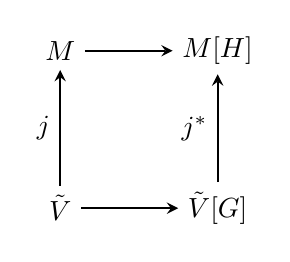
\begin{tikzpicture}[node distance=2cm]
			\node (M) {$M$};
			\node (MH) [right of=M] {$M[H]$};
			\node (V) [below of=M] {$\tilde{V}$};
			\node (VG) [right of=V] {$\tilde{V}[G]$};
			
			\draw [thick,->,>=stealth] (M) -- (MH);
			\draw [thick,->,>=stealth] (V) -- node [anchor=east] {$j$} (M);
			\draw [thick,->,>=stealth] (VG) --node [anchor=east] {$j^*$} (MH);
			\draw [thick,->,>=stealth] (V) -- (VG);
		\end{tikzpicture}
	\end{center}
\end{lemma}
\begin{proof}
	We define $j^*$ in the only way we can, and verify that the definition works. Let $S\in \tilde{V}[G]$ be a set. Let $\sigma$ be a $\PP$ name with $\sigma^G=S$. We fix
	
	$$j^*(S)=(j(\sigma))^H$$
	
	We must verify that $j^*$ is well defined. Suppose that $\sigma$ and $\tau$ are two $\PP$ names, and $\sigma^G=\tau^G$. Then there is some $p\in G$ such that $p\forces \sigma=\tau$. By elementarity $j(p)\forces j(\sigma)=j(\tau)$, and by assumption $j(p)\in H$. Hence $(j(\sigma))^H=(j(\tau))^H$.
	
	It is trivial to verify that $j^*$ extends $j$, and that the diagram commutes. The last thing to check is that $j^*$ is elementary, and this is done in a similar way to the ``well-defined" proof. Let $\varphi$ be a formula with parameters $\vec{S}=\vec{\sigma}^G$ and suppose that $\tilde{V}[G]\vDash \varphi(\vec{S})$. Then let $p\in G$ force $\varphi(\vec{\sigma})$; by elementarity $j(p)\forces \varphi(j(\vec{\sigma})$ and by assumption $j(p)\in H$. So $M[H]\vDash \varphi(j^*(\vec{S}))$.
\end{proof}

If we add some extra assumptions, we can also prove that $j^*$ preserves $\lambda$ sequences like a supercompact embedding.

\begin{lemma}
	Suppose the conditions of the above lemma hold, that $j(\PP)=\PP$, $H=G$ and that $\PP$ satisfies the $\lambda^+$ chain condition. Then $\tilde{V}[G]$ believes that $M[G]^\lambda \subset M[G]$.
\end{lemma}

In fact, this can be proved in much more general circumstances: rather than assuming that $j(\PP)=\PP$ and $H=G$ we only need that $G\in M[H]$ and $H\in \tilde{V}[G]$. But that's overkill for this proof.

\begin{proof}
	First, note that since $M$ is definable in $\tilde{V}$, $M[G]$ is definable in $V[G]$. Let $S=(S_\gamma)_{\gamma<\lambda}\in \tilde{V}[G]$ be a $\lambda$ sequence of elements of $M[G]$. Since $M$ and $G$ are definable in $\tilde{V}[G]$, we can also define a sequence $\dot{S}=(\dot{S}_\gamma)_{\gamma<\lambda}\in \tilde{V}[G]$ of names for the terms of $S$. (Note that $S$ itself is not a name, it's just a sequence of names.) Let $\dot{\Sigma}\in \tilde{V}$ be a $\PP$ name for $\dot{S}$. Let $p\in G$ force $\dot{\Sigma}$ to be a $\lambda$ sequence of $\PP$ names, each of which is an element of $M$.
	
	For $\gamma<\lambda$, let $A_\gamma$ be a maximal antichain of conditions below $p$ which decide which name $\dot{\Sigma}(\gamma)$ is going to be interpreted as. So for any $q\in A_\gamma$ there is some name $\sigma_{q,\gamma}\in M$ such that $q\forces \dot{\Sigma}(\gamma)=\sigma_{q,\gamma}$. Then $\dot{\Sigma}$ is forced by $p$ to be equal to
	
	$$\tau := \{\langle (\sigma_{q,\gamma},\check{\gamma}), q\rangle : \gamma<\lambda, q\in A_\gamma\}$$
	
	By the chain condition, $\lvert A_\gamma\rvert \leq \lambda$ for all $\gamma<\lambda$, and hence $\tau$ has cardinality $\leq \lambda$. All the elements of $\tau$ are in $M$, $\tau\in \tilde{V}$ and $M$ is closed under $\lambda$ sequences, so $\tau \in M$. So $\dot{S}=\tau^G\in M[G]$. The conclusion that $S\in M[G]$ is now immediate.
\end{proof}



%	\begin{lemma}\label{lemma M[H] closed under lambda sequences}
	%		Suppose the conditions of the above lemma hold, and that $\lambda$ is a cardinal of $\tilde{V}$ such that $\tilde{V}$ believes $M^\lambda \subset M$. Suppose also that $\PP$ satisfies the $\lambda^+$ chain condition over $\tilde{V}$, and that $G\in M[H]$. Then $\tilde{V}[G]$ believes $M[H]^\lambda\subset M[H]$.\footnote{My thanks to Philipp Schlicht for pointing out a mistake in the original version of this lemma.}
	%	\end{lemma}

%	This lemma is overkill for what we need at this point, but we'll need the full result later in the proof so we might as well get it out of the way now.

%	\begin{proof}
	%		First, note that since $j^*$ is an elementary embedding from $\tilde{V}[G]$ to $M[H]$, we know that $M[H]$ is contained in $\tilde{V}[G]$ and so the statement of the lemma makes sense.
	
	%		Suppose that $S=(S_\gamma)_{\gamma<\lambda}$ is a $\lambda$ sequence of elements of $M[H]$ which exists in $\tilde{V}[G]$. Working in $\tilde{V}[G]$, let $\dot{S}_\gamma \in M$ be a $j(\PP)$ name for $S_\gamma$ for each $\gamma<\lambda$. Let $\Sigma=(\dot{S}_\gamma)_{\gamma<\lambda}\in \tilde{V}[G]$ be the sequence of names. We can find a $\PP$ name $\dot{\Sigma}\in \tilde{V}$ for $\Sigma$: note that $\dot{\Sigma}$ is a $\PP$ name for a sequence of $j(\PP)$ names, each of which is an element of $M$. Choose $p\in G$ forcing that this is the case (which we can do, since $\tilde{V}$ can define $M$).
	
	%		For $\gamma<\lambda$, let $A_\gamma$ be a maximal antichain of conditions below $p$ such that every element of $A_\gamma$ decides which $j(\PP)$ name $\sigma\in M$ of $M$ $\dot{\Sigma}(\check{\gamma})$ is going to be equal to. So $q\in A_\gamma$ implies that $q\leq p$ and there is some $\sigma_{q,\gamma}\in M$ such that
	
	%		$$q\forces \dot{\Sigma}(\check{\gamma})=\check{\sigma}_{q,\gamma}$$
	
	%		Since $q\leq p$ we know that $\sigma_{q,\gamma}$ must be a $j(\PP)$ name.
	
	%		Let $\tau$ be the following $j(\PP)$ name, defined in $\tilde{V}$:
	
	%		$$\tau:=\Big\{\Big(\widecheck{(\gamma,x_{q,\gamma})},q\Big): \gamma<\lambda, q\in A_\gamma\Big\}$$
	
	%		We are assuming $\PP$ satisfies the $\lambda^+$ chain condition, so the cardinality of $\tau$ is $\lambda$. Moreover, all of its elements are in $M$. So $\tau \in M$.
	
	%		Hence, $\tau^G\in M[H]$. An easy forcing argument shows that $\tau^G$ is a $\lambda$ sequence of $j(\PP)$ names, and that for all $\gamma<\lambda$,
	
	%		$$\tau^G(\gamma)=\dot{\Sigma}^G(\gamma)=\Sigma(\gamma)=\dot{S}_\gamma$$
	
	%		Hence, $M[H]$ contains the sequence $\Sigma=(\dot{S}_\gamma)$, and so it also contains the sequence $(\dot{S}_\gamma^H) = (S_\gamma)$.
	%	\end{proof}
	
	\begin{corollary}
		$\kappa$ is supercompact in $V$.
	\end{corollary}
	\begin{proof}
		Let $\lambda>\kappa$. Let $j:V_0\rightarrow M$ be a $\lambda$ embedding: i.e. elementary, with critical point $\kappa$, $j(\kappa)>\lambda$ and $M^\lambda \subset M$. Let $G$ be the $\PP:=\col(\omega,\lvert \alpha \rvert)$ generic filter used in constructing $V$ (so $V=V_0[G]$). Note that $\PP$ is small compared to $\kappa$, so $j(\PP)=\PP$ and $G$ is also generic over $M$. Clearly for all $p\in G$, $j(p)=p\in G$. So $j$ extends to an elementary embedding $j^*: V_0[G]\rightarrow M[G]$ by the first lemma. Since $j^*$ extends $j$ it has critical point $\kappa$ and sends $\kappa$ up above $\lambda$. Since $\PP$ is small compared to $\kappa$ it certainly satisfies the $\lambda^+$ chain condition, and therefore by the second lemma $V=V_0[G]$ believes that $M[G]^\lambda \subset M[G]$.
	\end{proof}
	
	From now on, we will forget about $V_0$ and the collapsing forcing, and just work in $V$, a universe where $\alpha$ is countable, GCH holds and $\kappa$ is supercompact, and where $\Reg_{<\alpha}$ is unbounded. Note that since $\kappa$ is supercompact it is hyperinaccessible, and therefore $\Reg_{<\alpha}$ is also unbounded below $\kappa$. We will also assume (by cutting off the top of the model if necessary) that $\Reg_{\alpha}\setminus \kappa^+=\emptyset$. Note that $\kappa$ will be an inaccessible limit of elements of $\Reg_{<\alpha}$ (so it is in $\Reg_{\beta}$ for some $\beta>\alpha$), and by the assumption we just made it is the largest element of this $\Reg_{\beta}$.
	
	\subsection{The Structure of the Proof}
	
	We will construct a forcing which will make $\kappa$ the first element of $\Reg_{\alpha}$ and ensure $\LST(I,Q^\alpha),\LST(I,R^\alpha)\leq \kappa$. The actual forcing we want to use is complex to define -- it's a delicate combination of several other forcings, some of which are rather complicated in their own right. We'll start by giving an informal sketch of how the proof is going to work, before we dive into the technicalities.
	
	The forcing $\PP$ we use has three components. The first is a non-Mahlo forcing $\NM_\lambda$ which adds a club $C$ of singular cardinals below some cardinal $\lambda$. The second is a collapsing forcing $\col_\lambda$ which collapses all the cardinals below that $\lambda$, except for those which are a ``short distance'' above some element of $C$. This will leave $\lambda$ as the first element of $\Reg_{\alpha}$.
	
	The third component is a Prikry-style forcing $\QQ_\lambda$, for a cardinal $\lambda$. It adds an $\NM_\lambda$ generic club, adds a new \textit{condition} to the $\col_\lambda$ forcing, and singularises $\lambda$.
	
	$\PP$ will be an iteration of $\QQ_\lambda$ forcings (for strategically chosen $\lambda<\kappa$), followed by $\NM_\kappa$ and then $\col_\lambda$.
	
	This gives us a universe $V^\PP$ in which $\kappa$ is the first element of $\Reg_\alpha$. How do we show that $\LST(I,Q^\alpha), \LST(I,R^\alpha) = \kappa$? We already know that $\kappa\leq \LST(I,R^\alpha)\leq \LST(I,Q^\alpha)$ from the previous lemmas; we need to show that given any language $\mathcal{L}\in V^{\PP}$ (of cardinality $<\kappa$) and any $\mathcal{L}$ structure $\mathcal{A}\in V^{\PP}$, we can find a substructure of cardinality less than $\kappa$ which is $\mathcal{L}\cup(I,Q^\alpha)$-elementarily equivalent to $\mathcal{A}$. We use a similar approach to Theorem \ref{theorem LST maximum}.
	
	Say that $\mathcal{A}$ has cardinality $\mu\geq\kappa$. Because $\kappa$ is supercompact in $V$, we can find an embedding $j:V\rightarrow M$ such that $j(\kappa)>\mu$ and such that $\mu$ is only a ``short distance" above $\kappa$ (in the sense we were discussing a moment ago). With a good deal of effort, we can show that $\PP$ embeds nicely into $j(\PP)$, and that the conditions of 
	Lemma \ref{lemma j and j*} and Lemma \ref{lemma M[H] closed under lambda sequences} hold for some suitable $j(\PP)$ generic extension of $M$. For this to happen, we need the club of singulars added by $\NM_\kappa$ in $\PP$ to be an initial segment of the club of singulars added by $\NM_{j(\kappa)}$ in $j(\PP)$. So we need $\kappa$ to be singular. This is one of the reasons for introducing the Prikry-style forcing $\QQ_\lambda$: we will show that $j(\PP)$ contains $\QQ_\kappa$ and thus singularises $\kappa$. We will also need to ensure that the collapsing forcings in $\PP$ and $j(\PP)$ play nicely with each other.
	
	Now, in $M^{j(\PP)}$, we know that no cardinals between $\kappa$ and $\mu$ are collapsed or singularised, because $\mu$ is only a ``short distance'' above $\kappa$ and $\kappa$ is in the club of singulars added by $\NM_{j(\kappa)}$. And below $\kappa$ we can also show that $V^{\PP}$ and $M^{j(\PP)}$ agree about the cardinals and the regular cardinals. Hence, $\mathcal{L}\cup \{I,Q^\alpha\}$ interprets all statements about $\mathcal{A}$ in the same way in $V^{\PP}$ and $M^{j(\PP)}$. (There are some technicalities involved with dealing with $\kappa$ itself here, but they turn out not to be a problem.)
	
	From there, the proof follows that of Theorem \ref{theorem LST maximum}.
	
	So in summary, the proof will consist of the following steps:
	
	\begin{enumerate}
		\item Define a function $f$ that formalises the concept of ``a short distance''
		\item Define the non-Mahlo and collapsing forcings $\NM_\lambda$ and $\col_\lambda$ we discussed above
		\item Define the forcing $\QQ_\lambda$, which adds an $\NM_\lambda$ generic filter, adds a condition to $\col_\lambda$ and singularises $\lambda$
		\item Show that $\NM_\lambda * \col_\lambda$ embeds nicely in $\QQ_\lambda * \col_\lambda$
		\item Put these forcings together in some way to get the forcing $\PP$ we will be using
		\item Show that in a $\PP$ generic extension, the $\LST$ is number at most $\kappa$
	\end{enumerate}
	
	\subsection{Defining $f$}
	
	Recall the Laver function, for any supercompact cardinal $\kappa$:
	
	\begin{lemma*}\cite{laverMakingSupercompactnessIndestructible}
		There is a function $h:\kappa \rightarrow V_\kappa$ such that given any $x\in V$ and any $\mu \geq \kappa$, there is an $M$ with  $M^{\mu}\subset M$ and an embedding $j:V\rightarrow M$ with critical point $\kappa$, such that $j(\kappa)>\mu$ and $j(h)(\kappa)=x$.
	\end{lemma*}
	
	We use this $h$ to define a related function $f$ specifically for the ordinals.
	
	\begin{lemma}\label{lemma defining f}
		There is a strictly increasing function $f:\kappa\rightarrow \kappa$, whose range is a subset of $\Reg_\alpha$, such that:
		\begin{enumerate}
			\item For all $\gamma<\kappa$, the interval $(\gamma,f(\gamma))$ contains unboundedly many elements of $\Reg_\beta$ for every $\beta<\alpha$, but no elements of $\Reg_{\alpha}$
			\item For any $\mu>\kappa$, there is a model $M$ with $M^{\mu}\subset M$ and an elementary embedding $j:V\rightarrow M$ with critical point $\kappa$ such that $j(\kappa)>\mu$ and $j(f)(\kappa)>\mu$.
		\end{enumerate}
	\end{lemma}
	\begin{proof}For $\gamma<\kappa$, let $g(\gamma):=h(\gamma)$ if the latter is an ordinal greater than $\gamma$ but smaller than $\kappa$, and $(\gamma,g(\gamma) ) \cap \Reg_{\alpha}=\emptyset$, and otherwise let $g(\gamma):=\gamma$. Let $f(\gamma)$ be the least element of $\Reg_{\alpha}$ which is (strictly) above $g(\gamma)$. It is trivial to see that $f$ is strictly increasing and satisfies the first requirement.
		
		Fix $\mu>\kappa$. Using the previous result, let $M$ and $J:V\rightarrow M$ be such that $j(h)(\kappa)=\mu$. We know that $M$ is closed under $\mu$ sequences, so it correctly calculates the cardinalities and cofinalities of all cardinals below $\mu$. In particular, $\Reg_\alpha^M$ agrees with $\Reg_\alpha^V$ up to $\mu$, and hence $(\kappa,\mu)\cap \Reg_\alpha=\emptyset$ from the perspective of $M$. Hence $j(g)(\kappa)=j(h)(\kappa)=\mu$. So $j(f)(\kappa)>\mu$.
		
	\end{proof}
	
	In the language we used in the preamble to this proof, $\delta$ is ``a short distance" above $\gamma$ if $\delta \in (\gamma,f(\gamma))$.
	
	\subsection{NM and Col}
	Now we have $f$, we can define the simpler forcings used in this construction, $\NM_\lambda$ and $\col_\lambda$. Throughout this section, let $\tilde{V}$ be any universe which contains the $f$ we found in the previous section. We will also assume that $f$ has the same relation to $\Reg$ in $\tilde{V}$ as it does in $V$ (although we do \textit{not} assume that $\Reg_\beta^{\tilde{V}}=\Reg_\beta^V$ for any particular $\beta\leq \alpha$), and (in preparation for the future) we assume that GCH holds in $\tilde{V}$ except that there are perhaps a few singular cardinals $\lambda$ such that $2^\lambda=\lambda^{++}$. Let us fix $\lambda\leq \kappa$ to be a $\lambda^+$ supercompact cardinal in $\tilde{V}$.
	
	%In preparation for some technical work later, we will also fix some set $X\subset \lambda$ such that $(\Reg_\alpha\setminus X)\cap \lambda$ is unbounded below $\lambda$.
	
	A Mahlo cardinal is one for which the class of regulars below it is stationary, so to stop it being Mahlo we need to add a club which consists only of singular cardinals. We use a variant of the usual club shooting forcing which also chooses some elements of $\Reg_\alpha$.
	
	\begin{definition}
		We define the non-Mahlo forcing $\NM_\lambda$ as follows. Its elements are closed bounded subsets of $\lambda$, whose minimum element is $\omega$, whose successors are all taken from $\Reg_{\alpha}$, and whose limits are all singular. We order $\NM_\lambda$ by end inclusion.
	\end{definition}
	
	Note that this is not quite the usual non-Mahlo forcing: it gives us a club whose \textit{limits} are singular, but whose successors are elements of $\Reg_{\alpha}$. (Since $\Reg_\alpha$ is unbounded below $\lambda$, we do get an unbounded subset of $\lambda$ despite the odd requirement for successors.) By contrast, a standard non-Mahlo forcing would just add a club of singular cardinals. Of course, we can obtain a fully singular club here simply by deleting all the successors, so $\NM_\lambda$ does indeed force that $\lambda$ is no longer Mahlo.
	
	Although $\NM_\lambda$ is not strictly $<\lambda$ closed (since the limit of a sequence of conditions could be inaccessible) it is almost $<\lambda$ closed, and we can prove the usual results of $<\lambda$ closed-ness.
	
	\begin{lemma}
		Let $\mu<\lambda$. Then there are densely many conditions $p$ such that $\NM_\lambda {\upharpoonleft} p$ is $\mu$ closed.
	\end{lemma}
	\begin{proof}
		Let $p\in \NM_\lambda$ be any condition whose final element is larger than $\mu$. Let $p\geq p_0\geq p_1\geq \ldots$ be a descending sequence of conditions of length $\mu$. Then $p_0 \subset p_1 \subset \ldots$ are all end extensions of one another, so $\bigcup_{i<\mu}p_i$ is a set whose successors are all in $\Reg_\alpha$ and whose limit \textit{elements} are all singular. It is closed, except that it might not contain its supremum $\gamma$. But $\gamma\geq \sup p>\mu$ has cofinality $\cof(\mu)$, so it is singular. This implies that $\gamma<\lambda$, and that $\bigcup_{i<\mu}p_i \cup \{\gamma\}\in \NM_\lambda$.
	\end{proof}
	
	\begin{corollary}\label{corollary basic facts about NM}
		$\NM_\lambda$ is $<\lambda$ distributive, does not collapse or singularise any cardinals, and preserves GCH, except perhaps that $2^\lambda$ becomes $\lambda^{++}$.
	\end{corollary}
	\begin{proof}
		Let $\mu<\lambda$. Let $D_i: i<\mu$ be a collection of dense sets. Fix some $p$ such that $\NM_\lambda {\upharpoonleft} p$ is $\mu$ closed. For $i<\mu$ let $D_i'=D_i\cap (\NM_\lambda {\upharpoonleft} p)$. Then $D_i'$ is a dense subset of $\NM_\lambda{\upharpoonleft} p$. We know that $\NM_\lambda {\upharpoonleft} p$ is $\mu$ distributive since it is $\mu$ closed, and hence $\emptyset \neq \bigcap D_i'\subset \bigcap D_i$.
		
		It follows immediately from distributivity that $\NM_\lambda$ preserves all cardinals $<\lambda$ and does not singularise any of them, and that it preserves GCH below $\lambda$.
		
		Showing that $\lambda$ is not collapsed or singularised requires a slightly more technical argument, imitating the standard proof we'd use for a $\lambda$ closed forcing. Suppose that $\tilde{V}[G]$ collapses $\lambda$. Let $g:\mu\rightarrow \lambda$ be a bijection for some $\mu<\lambda$, and let $\dot{g}$ be a name for $g$. Let $p \in G$ force ``$\dot{g}$ is a bijection from $\mu$ to $\lambda$". Let $q\leq p$ be such that $\NM_\lambda {\upharpoonleft} q$ is $\mu$ closed. We construct a descending sequence of conditions $q = q_0\geq q_1\geq \ldots$ (not necessarily elements of $G$) of length $\mu+1$ as follows. If $i=j+1$ then we choose $q_i\leq q_j$ which decides the value of $\dot{g}(j)$. If $i$ is a limit, then by $\mu$ closed-ness, we can choose some $q_i$ below every earlier $q_j$. At the end, $q_\mu$ has decided $\dot{g}(i)$ for every $i$, and hence has defined a bijection from $\mu$ to $\lambda$ in $\tilde{V}$. Contradiction. A similar proof shows that $\lambda$ is not singularised.
		
		Finally, note that $\NM_\lambda \subset \lambda^{<\lambda}$, so
		
		$$\lvert \NM_\lambda \rvert \leq \sum_{\gamma<\lambda} \lambda^\gamma = \sum_{\gamma<\lambda}\lambda=\lambda$$
		
		Hence $\NM_\lambda$ has the $\lambda^+$ chain condition, and so does not collapse or singularise any cardinals $\geq \lambda^+$, and preserves GCH for cardinals above $\lambda$.
		
		Finally, then, in the generic extension $2^\lambda\leq 2^{\lambda^+}=\lambda^{++}$.
	\end{proof}
	
	Throughout this proof, we shall write $C$, and variants thereof, to refer to the generic club added by $\NM_\lambda$. It should (hopefully) always be clear from context to which $\lambda$ we are referring. Notice that for any $\gamma\in C$, we know $\Succ(\gamma)\geq f(\gamma)$, because there are no $\Reg_{\alpha}$'s between $\gamma$ and $f(\gamma)$.
	
	Next, we define the collapsing forcing. Recall that if $\gamma$ is regular and $\delta$ is strongly inaccessible, the forcing $\col(\gamma,<\delta)$ collapses all the cardinals between $\gamma$ and $\delta$ down to $\gamma$.
	
	For the rest of this section, let us fix a club $C$ which is generic for $\NM_\lambda$. We will work in some generic extension $\tilde{V}[G]$ of $\tilde{V}$ containing $C$, but we \textit{do not} assume that $\tilde{V}[G]=\tilde{V}[C]$. We will, however, assume that $G$ does not collapse or singularise any cardinals below $\lambda$, and preserves GCH below $\lambda$. In particular, this means that all the successors of $C$ will be strongly inaccessible in $\tilde{V}[G]$. The reason for this slightly arcane scenario is that we will eventually need to have definitions for $\col_\lambda$ in two different universes: $\tilde{V}^{\NM_\lambda}$, and $\tilde{V}^{\QQ_\lambda}$. We have already seen that $\NM_\lambda$ preserves GCH; once we define $\QQ_\lambda$ we will discover that it also preserves GCH below $\lambda$.
	
	The forcing we want to work with is a combination of these collapsing forcings, and is defined in terms of $C$. We want a forcing which will collapse, for each $\gamma \in C$, every cardinal between $f(\gamma)$ and $\Succ_C(\gamma)$. Once we have done this, it will be easy to see that it makes $\lambda$ the first element of $\Reg_{\alpha}$. The forcing we want to use is the Easton product of all the collapsing forcings:
	
	\begin{definition}
		Let $\tilde{V}[G]$ be some generic extension of $\tilde{V}$, which contains an $\NM_\lambda^{\tilde{V}}$ generic club $C$, and preserves GCH below $\lambda$. We define the forcing $\col_\lambda$ to be the set of all the elements $h$ of
		
		$$\prod_{\gamma\in C} \col(f(\gamma),<\Succ_C(\gamma))$$
		
		such that for all regular cardinals $\mu \leq \lambda$, the set
		
		$$\{\gamma \in C\cap \mu : h(\gamma)\neq \emptyset\}$$
		
		is bounded in $\mu$.
		
		We order $\col_\lambda$ in the obvious way.
	\end{definition}

Note that $\col_\lambda$ depends critically on our choice of $\NM_\lambda$ generic club $C$. So really, we should include $C$ as a subscript. But there will never be more than a single generic club below $\lambda$, so we will leave this implicit.

$\col_\lambda$ also depends on which cardinals are regular. So even if two universes both contain the same generic club $C$, we may find that $\col_\lambda$ is different. In particular, once we have defined $\QQ_\lambda$ we will find that $\col_\lambda$ will be different in $\tilde{V}^{\NM_\lambda}$ and $\tilde{V}^{\QQ_\lambda}$, even if both generic extensions add the same club.
	
	If $c$ is a closed subset of $\lambda$, then we extend the above definition by defining $\col(c)$ in the obvious way, as the Easton support product of $\col(f(\gamma),<\Succ_c(\gamma))$ forcings for $\gamma\in c \setminus \max(c)$. If $c\in \tilde{V}$ then this can be defined in the ground model $\tilde{V}$, before we add an $\NM_\lambda$ generic club $C$. Of course, once we do add $C$, we know that if $c$ is an initial segment of $C$ then $\col(c)$ will be a subset of $\col(C)=\col_\lambda$. (Technically, this is only true if we allow a minor abuse of notation about the domains of the functions in $\col(c)$ and $\col_\lambda$.)
	
	\begin{proposition}\label{proposition col(c) closed}
		Let $c$ be a closed set of cardinals (in $\tilde{V}$ or $\tilde{V}[G]$) whose successors are all inaccessibles below $\kappa$. If $\gamma=\min(c)$ then $\col(c)$ is $<f(\gamma)$ closed in any universe where this makes sense. In particular, this means it is $\gamma^+$ closed.
	\end{proposition}
	\begin{proof}
		An easy definition chase we leave to the reader.
	\end{proof}
	
	
	\begin{lemma}\label{lemma basic facts about col}
		In any universe where $\col_\lambda$ is defined (i.e. any universe containing an $\NM_\lambda$ generic club $C$ whose successors are strongly inaccessible), it does not collapse any cardinals except those which it is supposed to (i.e. those in the interval $(f(\gamma), \Succ_C(\gamma))$ for some $\gamma \in C$). Nor does it singularise any other cardinals.
	\end{lemma}
	\begin{proof}
		Let $\mu$ be a cardinal which is not in any of the intervals that are supposed to be collapsed by $\col_\lambda$. Let $\PP=\col(C {\upharpoonleft} \mu)$ (in the sense of $\tilde{V}[C]$, not $\tilde{V}$) and let $\RR=\col(C\setminus \mu)$. Then $\col_\lambda=\PP\times \RR$. Now $\PP$ has cardinality less than $\mu$ (by GCH) and therefore does not collapse or singularise $\mu$. On the other hand, $\RR$ is $\mu$ closed, and so again it does not collapse or singularise $\mu$.
	\end{proof}
	
	\begin{corollary}
		In any universe where $\col_\lambda$ is defined, if $0<\beta<\alpha$ then $\col_\lambda$ does not modify $\Reg_\beta$, other than removing those elements which are in an interval $(f(\gamma),\Succ_C(\gamma))$.
	\end{corollary}
	\begin{proof}
		Let $\mu\in \Card$ not be in $(f(\gamma),\Succ_C(\gamma))$ for any $\gamma \in C$. We show that $\mu\in \Reg_\beta$ in the $\col_\lambda$ generic extension if and only if $\mu \in \Reg_\beta$ in $\tilde{V}[G]$.
		
		Case 1: $\mu<\min(C)$, $\mu \in (\gamma,f(\gamma)]$ or $\mu>\lambda$. All the cardinals in these intervals are preserved, and not singularised, by $\col_\lambda$. So $\Reg_\beta$ is preserved over these intervals too.
		
		Case 2: $\mu \in C$ is a successor of $C$. By definition of $\NM_\lambda$, we know $\mu$ is an element of $\Reg_\alpha$ in $\tilde{V}[G]$, and hence not in $\Reg_\beta$. In the generic extension $\mu$ becomes a successor cardinal, and hence again not in $\Reg_\beta$.
		
		Case 3: $\mu \in C$ is a limit of $C$. By definition of $\NM_\lambda$, we know $\mu$ is a successor cardinal in $\tilde{V}[G]$ and hence also in the $\col_\lambda$ generic extension.
		
		Case 4: $\mu=\lambda$. In $\tilde{V}$, we know that $\lambda>\beta$ is hyperinaccessible, and therefore a limit of elements of $\Reg_\beta$. By assumption, $\tilde{V}[G]$ agrees with $\tilde{V}$ on $\Reg{\upharpoonleft} \lambda$, so in particular in $\tilde{V}[G]$ we know that $\lambda$ is still a limit of $\Reg_{\beta}$. So it cannot be an element of $\Reg_\beta$. Recall that every interval $(\gamma,f(\gamma)]$ contains an element of $\Reg_\beta$. So by Case 1, we know that in the generic extension $\lambda$ is still a limit of elements of $\Reg_\beta$, and hence cannot be in $\Reg_\beta$.
	\end{proof}	
	
	Notice also that in the $\col_\lambda$ generic extension, there are no elements of $\Reg_\alpha$ below $\lambda$, and that $\lambda$ is a limit of elements of $\Reg_\beta$ for all $\beta<\alpha$. So if $\lambda$ is regular in $\tilde{V}[G]$ (and hence in the $\col_\lambda$ generic extension) then it will be the first element of $\Reg_\alpha$.
	
	\subsection{The Prikry-style forcing Q}
	
	Again, we fix a $\lambda^+$ supercompact $\lambda\leq\kappa$ in a universe $\tilde{V}$ which knows about $f$.% Assume also that $\col(C)$ is well defined for every $\NM_\lambda^{\tilde{V}}$ generic club $C$.
	
	The forcing $\QQ_\lambda$ is similar to a Prikry forcing, but with some extra components. We want any $\QQ_\lambda$ generic filter to not only singularise $\lambda$, but also to define a $\NM_\lambda$ generic club $C$. For reasons that will become clearer later, we also want it to define some kind of ``generic \textit{element}" of $\col_\lambda$.
	
	Where a standard Prikry forcing would add an $\omega$ sequence of single ordinals, we will arrange for $\QQ_\lambda$ to add an $\omega$ sequence whose terms are taken from the following set:
	
	\begin{definition}
		$K_\lambda$ is the set of all triples $\langle c,x,\epsilon\rangle$ where:
		\begin{enumerate}
			\item $c\in \NM_\lambda$;
			\item $h\in \col(c)$;
			\item $\epsilon \in \On$ and $\max(c)<\epsilon<\lambda$.
		\end{enumerate}
		
		For $\beta<\lambda$, $K_\lambda^\beta$ is the subset of $K_\lambda$ consisting of all the triples $\langle c,h,\epsilon \rangle$ where the least element of $c$ is greater than $\beta$ (and thus also $\epsilon>\beta$).
	\end{definition}
	
	The Prikry-style generic sequence we're aiming for will consist of an element $\langle c_0,h_0,\epsilon_0 \rangle$ of $K_\lambda$, then an element $\langle c_1,h_1,\epsilon_1 \rangle$ of $K_\lambda^{\epsilon_0}$, and so on up through the all $n\in\omega$.
	
	From such a sequence $G$, we will be able to extract a club $C=\bigcup_{n\in \omega} c_n$ in $\lambda$, an element $H=\bigcup_{n\in \omega} h_n$ of $\prod_{\gamma\in C} \col(\gamma,<\Succ_C(\gamma))$ and an $\omega$-sequence $(\epsilon_n)$. If we set up the forcing correctly, we will later discover that $C$ is $\NM_\lambda$ generic, that $H\in \col^{\tilde{V}[G]}_\lambda$, and that $(\epsilon_n)$ is cofinal in $\lambda$.
	
	Recall that a condition in a Prikry forcing consists of two components: a finite stem of the sequence we're constructing, and a ``large" (i.e. measure $1$) set of places that are allowed to be in later parts of the sequence.
	
	It's fairly easy to see what the finite stem should look like in this context. But how can we find an analogue of a measure $1$ set of ordinals? We must define a measure on $K_\lambda$, and in fact on $K_\lambda^\beta$ for every $\beta<\lambda$.
	
	To do this, we first define an ordering on $K_\lambda$:
	
	\begin{definition}
		Let $\langle c,h,\epsilon\rangle$ and $\langle \tilde{c},\tilde{h},\tilde{\epsilon}\rangle$ be elements of $K_\lambda$. We say that $\langle\tilde{c},\tilde{h},\tilde{\epsilon}\rangle\leq^* \langle c,h,\epsilon\rangle$ if:
		
		\begin{enumerate}
			\item $\tilde{c}\leq c$, that is, $\tilde{c}$ is an end extension of $c$;
			\item $\tilde{h}{\upharpoonleft} \max(c) = h$;
			\item $\tilde{\epsilon}\geq \epsilon$.
		\end{enumerate}
	\end{definition}
	
	Notice the unusual nature of the second clause. It's not enough that $\tilde{h}\leq h$ in the $\col(\tilde{c})$ ordering. It must actually agree completely with $h$, although it is allowed to add more things once we're above the area where $h$ is defined. This is because $H=\bigcup h_n$ is supposed to be a \textit{condition} in $\col_\lambda$, not a $\col_\lambda$ generic filter.
	
	Of course, this also defines an ordering on $K_\lambda^\beta\subset K_\lambda$ for every $\beta<\lambda$.
	
	\begin{lemma}
		Let $\beta<\lambda$. Let $F$ be the family of all subsets of $K_\lambda^\beta$ which contain a $\leq^*$ dense open subset of $K_\lambda^\beta$. Then $F$ is a $\lambda$ complete filter in $K_\lambda^\beta$ in the usual $\subset$ ordering of $\mathcal{P}(K_\lambda^\beta)$.
	\end{lemma}
	\begin{proof}
		Clearly, $F$ is upwards closed and nonempty. The intersection of fewer than $\lambda$ many $\leq^*$ dense open sets can be easily seen to be dense open, so $F$ is a $\lambda$ complete filter.
	\end{proof}
	
	The following is a standard consequence of $\lambda^+$ supercompactness:
	
	\begin{lemma}\cite[22.17]{kanamori}
		Let $S$ be a set of size $\lambda$, and let $F$ be a $\lambda$ complete filter on $\mathcal{P}(S)$. Then $F$ can be extended to a $\lambda$ complete ultrafilter $U$.
	\end{lemma}
	\begin{proof}
		Without loss of generality, let us assume $S=\lambda$. Note that $\lvert F\rvert \leq 2^\lambda=\lambda^+$. Let $j:\tilde{V}\rightarrow M$ be an embedding with critical point $\lambda$ such that $j(\lambda)>\lambda^+$ and $M^{\lambda^+}\subset M$. By elementarity $j(F)\in M$ is $j(\lambda)$ complete. Since $\lvert j''(F)\rvert\leq \lambda^+$ (in $\tilde{V}$) and $M$ is closed under $\lambda^+$ sequences, we know that $j''(F)\in M$. Since also $\lambda^+\leq j(\lambda)$ and $j''(F)\subset j(F)$, we know by $j(\lambda)$ completeness of $j(F)$ that $\cap j''(F) \in j(F)$. In particular, there is some $\gamma\in \cap j''(F)$. Now define an ultrafilter $U \in \tilde{V}$ by:
		
		$$X\in U \iff X\subset \lambda \wedge \gamma \in j(X)$$
		
		It is easy to check that $F\subset U$, that $U$ is an ultrafilter, and that it is $\lambda$ complete.
	\end{proof}
	
	\begin{corollary}
		Let $\beta<\lambda$. There is an ultrafilter $U_\beta$ on $K_\lambda^\beta$ which contains all the $\leq^*$ dense open subsets of $K_\lambda^\beta$.
	\end{corollary}
	
	In fact, of course, there will be many such ultrafilters, but we will fix a single one for the rest of this section to call $U_\beta$.
	
	With $U_\beta$ in hand, we can define the analogue of the measure $1$ set of ordinals in a Prikry forcing.
	
	\begin{definition}
		Let $T$ be a tree of height $\omega$, whose nodes are all elements of $K_\lambda$. We abuse notation by allowing the same element of $K_\lambda$ to appear multiple times, provided no element appears twice as direct successors of the same node. We say $T$ is \textit{nice} if the following hold:
		
		\begin{enumerate}
			\item If $\langle \tilde{c},\tilde{h},\tilde{\epsilon}\rangle <_T \langle c,h,\epsilon\rangle\in T$, then $\langle \tilde{c},\tilde{h},\tilde{\epsilon}\rangle\in K_\lambda^\epsilon$;
			\item If $\langle c,h,\epsilon \rangle \in T$ then the set of its direct successors (which is a subset of $K_\lambda^\epsilon$ by the previous condition) is in $U_\epsilon$.
		\end{enumerate}
	\end{definition}
	
	Recall that a condition in a Prikry forcing contains two components: a finite sequence of ordinals, and a measure $1$ set. The finite sequence fixes an initial segment of the $\omega$ sequence we are going to add, and the rest of the sequence is chosen from elements of the measure $1$ set. Analogously, in the forcing $\QQ_\lambda$, our conditions will have two components: a finite sequence $s$ of terms from $K_\lambda$ and a nice tree $T$ which gives us a map of where the sequence is allowed to go from there. The root of $T$ will the final term of $s$. Then for $n>0$, the $n$'th level contains all the elements of $K_\lambda$ which we are allowing to appear as the $n$'th term in the \textit{undetermined} part of the sequence. A branch through the tree corresponds to a (not necessarily generic) way to complete the sequence.
	
	\begin{definition}
		The forcing $\QQ_\lambda$ has conditions of the form
		
		$$\big((\langle c_0,h_0,\epsilon_0\rangle, \langle c_1,h_1,\epsilon_1\rangle,\ldots,\langle c_{n-1},h_{n-1},\epsilon_{n-1}\rangle),T\big)$$
		
		for some $n\in \omega$, where
		
		\begin{enumerate}
			\item $\langle c_0,h_0,\epsilon_0\rangle \in K_\lambda$ if $n>0$;
			\item For $0<i<n$, $\langle c_i,h_i,\epsilon_i\rangle \in K_\lambda^{\epsilon_{i-1}}$;
			\item $T$ is a nice tree
			\item The root of $T$ is $\langle c_{n-1},h_{n-1},\epsilon_{n-1}\rangle$.
		\end{enumerate}
		
		We call $\epsilon_{n-1}$ the height of the condition (writing $\height$ in symbols).
		
		The conditions are ordered in the usual way for a Prikry style forcing: $(s',T') \leq (s,T)$ if $s'$ is an end extension of $s$ and there is a path $B=b_0,b_1,\ldots,b_k$ through $T$ of length $k:=\lvert s'\setminus s\rvert+1$ such that:
		\begin{enumerate}
			\item $b_0$ is the root of $T$ (i.e. the last element of $s$)
			\item For all $0<i\leq k$, $b_i$ is the $i$'th element of $s'\setminus s$
			\item $T'$ is a subtree of $T$ whose root is $b_k$
		\end{enumerate}
		
		As usual for Prikry forcings, if $s'=s$ we say $(s',T')$ is a direct extension of $(s,T)$ and write $(s',T')\leq^*(s,T)$.
	\end{definition}
	
	Note: We now have two different definitions of $\leq^*$. One talks about elements of $K_\lambda$ and the other about conditions in $\QQ_\lambda$, so it should be easy to understand which one we are talking about.
	
	\begin{proposition}\label{proposition Qlambda quasi closed}
		The forcing $(\QQ_\lambda, \leq^*)$ is ${<}\lambda$ closed. That is, any descending sequence $T_0\supset T_1\supset T_2\ldots$ of nice trees with the same root will have a nice tree as their intersection.
	\end{proposition}
	\begin{proof}
		Follows from the fact that $U_\epsilon$ is closed under $<\lambda$ intersections.
	\end{proof}
	
	\noindent The following lemma is very standard for Prikry style forcings.
	
	\begin{lemma}
		Let $p\in \QQ_\lambda$. Let $\varphi$ be first order (perhaps with parameters). Then there is some $q\leq^* p$ deciding $\varphi$.
	\end{lemma}
	\begin{proof}
		We'll essentially follow the standard proof of this result for Prikry forcings. However, the argument gets rather technical to state, because we need to construct a tree analogue of the diagonal intersection of measure $1$ sets. The way we do this is really quite simple and natural, but unfortunately it's also rather messy to write out.
		
		Let $p=(s,T)$. We shall recursively construct a condition $r=(s,T')\leq^* p$, together with a collection of nice subtrees $\{T_t \subset T: t \in T'\}$, where $T_t$ has root $t$. For $t\in T'$, we define $s_t$ to be the sequence of predecessors of $t$ in $T'$, starting at the root of $T'$ and ending at $t$ itself. For each $t\in T'$, the intention is that $(s\cup s_t,T'{\upharpoonleft} t)$ should be a condition of $\QQ_\lambda$ below $(s\cup s_t,T_t)$; and that if at all possible both will decide $\varphi$.
		
		First, suppose $t$ is the root of $T$ (which will also have to be the root of $T'$, since $(s,T')$ is supposed to be a condition of $\QQ_\lambda$). If there is some $r_t\leq^* p$ which decides $\varphi$, then let $T_t$ be its associated tree. (Of course, if such an $r_t$ exists, then we're already done!). Otherwise, let $T_t=T$.
		
		Now, let $n>0$ and assume that we have already defined levels $1\ldots,n$ of $T'$, as well as $T_t$ for all $t$ in these levels of $T'$. Let $t\in T'$ be at level $n$. Then we define the direct successors of $t$ in $T'$ to be the level $1$ elements of $T_t$ (all of which are, by inductive hypothesis, direct successors of $t$ in $T$). In doing this, we have define the whole of level $n+1$ of $T'$. It remains to define the trees $T_u$ of elements $u$ of this level.
		
		If $u\in T'$ is a direct successor of $t$, then let $T_u^0$ be the restriction $T_t{\upharpoonleft} u$ of $T_t$ to $u$. (So $T_u^0$ has root $u$ and consists of all elements of $T_t$ which are below $u$.) Consider the condition $p_u:=(s \cup s_u, T_u^0)$. Since $u\in T$ and $T_t$ is a subtree of $T$, we know that $p_u\leq p$. If there is some direct extension $r_u \leq^* p_u$ which decides $\varphi$, then let $T_u$ be the tree in $r_u$. If no such $r_t$ exists, then we define $T_u:=T_u^0$. This completes the recursive definition.
		
		It is easy to verify that $r:=(s,T')\leq^* p$, and that it has the following property: if $\tilde{r}=(\tilde{s},\tilde{T})\leq r$ decides $\varphi$, then so does $(\tilde{s},T' {\upharpoonleft} \max\tilde{s})$.
		
		The next step is to recursively construct another condition $q=(s,T'')\leq^* r$ which actually decides $\varphi$ itself. This time, the construction is a little simpler: we don't need the auxiliary $T_t$ trees. The root of $T''$ is the same as that of $T'$ and $T$, of course.
		
		Say that we have built the first $n$ levels of $T''$. Let $t$ be in the $n$'th level of $T''$, and let $A\subset K_\lambda$ be the set of all its direct successors in $T'$. Recall that $A$ is measure $1$ in the sense of $U_\beta$, where $\beta$ is the height of $t$. We partition $A$ into three parts: we say that $u\in A$ is in $A_1$ if $q_u := (s \cup s_u, T' {\upharpoonleft} u)$ decides that $\varphi$ is true, $u$ is in $A_2$ if $q_u$ decides $\varphi$ is false, and $u$ is in $A_3$ if $q_u$ doesn't decide $\varphi$ at all.
		
		One of $A_1$, $A_2$ and $A_3$ will be measure $1$ in the sense of $U_\beta$. The direct successors of $t$ in $T''$ are defined to be the elements of that measure $1$ set. It is again easy to verify that this defines a nice tree $T''$ and that $q:=(s,T'')\in \QQ_\lambda$. It is also easy to check that $q\leq^* r\leq^* p$ and that $q$ has the following two properties:
		\begin{enumerate}
			\item If $\tilde{q}=(\tilde{s},\tilde{T})\leq q$ decides $\varphi$, then so does $q':=(\tilde{s},T'' {\upharpoonleft} \tilde{s})$ (this follows from $q\leq r$); and
			\item For any extension $q'=(\tilde{s}, T'' {\upharpoonleft} \tilde{s})$ of $q$, either all the one step extensions of $q'$ fail to decide $\varphi$, or they all decide it and make the same decision.
		\end{enumerate}
		
		Let $\tilde{q}=(\tilde{s}, \tilde{T}) \leq q$ be some condition which decides $\varphi$, and let it be such that $\tilde{s}$ has minimal length among conditions which decide $\varphi$. Then by the first property, $\varphi$ is decided by $q':=(\tilde{s},T'' {\upharpoonleft} \tilde{s})$. Suppose, seeking a contradiction, that $\tilde{s}$ is a proper extension of $s$, and let $\tilde{s}'$ be $\tilde{s}$ with its final term $t$ omitted. (So by assumption, $\tilde{s}'$ still extends $s$.)
		
		Then $q'$ is a one step extension of $q'':=(\tilde{s}',T''{\upharpoonleft} \tilde{s}')$, and decides $\varphi$. So by the second property, all the one-step extensions of $q''$ decide $\varphi$, and agree on that decision. But then $q''$ decides $\varphi$ as well, and this is a contradiction since $\tilde{s}'$ is shorter than $\tilde{s}$.
		
		So in fact $\tilde{s}=s$ and $\tilde{q}\leq^* q$ decides $\varphi$.
	\end{proof}
	
	\begin{corollary}
		Let $\varphi(x)$ be a formula with one free variable, let $\mu\leq\lambda$, and let $p\forces \exists x<\check{\mu} \,\varphi(x)$. Then there is some $q\leq^* p$ and some $\gamma <\mu$ such that $q\forces \varphi(\check{\gamma})$.
	\end{corollary}
	\begin{proof}
		If no such $q$ exists, then let $p=q_0\geq^*q_1\geq^*q_2\ldots$ be a descending sequence of conditions of length $\mu+1$ defined as follows. For $i=j+1$, we choose $q_i\leq^*q_j$ deciding $\varphi(\check{j})$; by assumption $q_i\forces \neg \varphi(\check{j})$. At limit $i$ we take some $q_i$ which is $\leq^*$ every $q_j, j<i$. This exists by $<\lambda$ closure of $(\QQ_\lambda,\leq^*)$. Then $q_\mu\leq^* p\forces \forall x<\check{\nu} \neg \varphi(x)$. Contradiction.
	\end{proof}
	
	This tells us that $\QQ_\lambda$ does not do any unexpected collapsing or singularising of cardinals.
	
	\begin{lemma}\label{lemma facts about Qlambda}
		$\QQ_\lambda$ does not add any new bounded subsets of $\lambda$, collapse any cardinals, or singularise any cardinals apart from $\lambda$. It preserves GCH where it holds in $\tilde{V}$, except at $\lambda$.
	\end{lemma}
	\begin{proof}
		First, note that $\QQ_\lambda$ has the $\lambda^{+}$ chain condition, because any two conditions of $\QQ_\lambda$ with the same stem are compatible. Hence, it does not collapse or singularise any cardinals $\geq\lambda^+$, or change the cardinalities of their power sets.
		
		Let $\mu< \lambda$ be a cardinal of $\tilde{V}$, and suppose that $\QQ_\lambda$ collapses it to some cardinal $\nu<\mu$. Let $\dot{g}$ be a name for a bijection $g:\nu\rightarrow \mu$. Let $p\forces \dot{g}: ``\check{\nu}\rightarrow \check{\mu} \text{ is a bijection}"$. We construct a descending chain of direct extensions $p=p_0\geq^*p_1\geq^*\ldots$ of length $\nu+1$. If $i$ is a successor, then we use the previous corollary to take $p_i$ deciding the value of $\dot{g}(i)$; at limit $i$ we take some $p_i$ which is $\leq^*p_j$ for all $j<i$. Then $p_\nu$ decides what $g$ is, and hence $g\in \tilde{V}$. Contradiction. A similar proof shows that $\QQ_\lambda$ does not singularise $\mu$ either, and that it adds no bounded subsets of $\lambda$. (For the latter, we start with some $p\in \QQ_\lambda$ which decides what the bound will be, and then take a $\leq^*$ descending chain whose length is that bound, deciding which elements of $\lambda$ will be in the new subset.)
		
		This also means that $\lambda$ is a limit of cardinals in $\tilde{V}[G]$, and hence is still a cardinal, and that the power sets of cardinals below $\lambda$ are preserved.
	\end{proof}
	
	
	All our definitions of $\NM_\lambda$, $\col_\lambda$ and $\QQ_\lambda$ have been given only for $\lambda\leq \kappa$. The only reason for this is because we use $f$ in their definition, and $f$ is only defined up to $\kappa$. We will later want to deal with elementary embeddings $j:\tilde{V}\rightarrow M$ with critical point $\kappa$. From the perspective of such a model $M$, we can extend the definition by introducing analogous forcings in terms of $j(f)$, for any $\lambda \leq j(\kappa)$. We will extend the notation by referring to these forcings also as $\NM_\lambda$, $\col_\lambda$ and $\QQ_\lambda$. Since $j(f)$ will be an end-extension of $f$, for $\lambda\leq \kappa$ the forcings $\NM_\lambda$, $\col_\lambda$ and $\QQ_\lambda$ are defined the same way in $M$ whether we use $f$ or $j(f)$ in their definitions, so there is no ambiguity in doing this.
	
	\subsection{Embedding NM*Col into Q*Col}
	
	Once again, fix a $\lambda^+$ supercompact $\lambda\leq \kappa$ in a universe $\tilde{V}$ which knows about $f$. % and $X\subset \lambda$ such that $\Reg_\alpha \setminus X$ is unbounded in $\lambda$.
	As we discussed earlier, we can extract elements of $\NM_\lambda$ and $\col_\lambda$ from a $\QQ_\lambda$ condition.
	
	\begin{definition} We define two schemes of abbreviations.
		
		\begin{enumerate}
			\item Let
			$$p=((\langle c_0,h_0,\epsilon_0\rangle, \langle c_1,h_1,\epsilon_1\rangle,\ldots,\langle c_{n-1},h_{n-1},\epsilon_{n-1}\rangle),T)$$
			be a condition in $\QQ_\lambda$. We define $c_p=\bigcup_{i<n} c_i$ and $h_p=\bigcup_{i<n}h_i$.
			\item Let $G$ be $\QQ_\lambda$ generic. We define $C_G=\bigcup_{p\in G} c_p$ and $H_G=\bigcup_{p\in G} h_p$.
		\end{enumerate}
	\end{definition}
	
	An equivalent, but less friendly, definition is that
	
	$$C_G=\bigcup \{c: \exists h, \epsilon \,\, \langle c,h,\epsilon\rangle \text{ is a term in the first part of some } p\in G\}$$
	and that
	$$H_G=\bigcup \{h: \exists c, \epsilon \,\, \langle c,h,\epsilon\rangle \text{ is a term in the first part of some } p\in G\}$$
	
	We shall now establish what these four objects actually are, in terms of $\NM_\lambda$ and $\col_\lambda$. The first two objects, $c_p$ and $h_p$, are simply conditions of the relevant forcings in $\tilde{V}$:
	
	\begin{proposition}\label{proposition c_p h_p}
		Let $p\in \QQ_\lambda$. Then $c_p\in \NM_\lambda$ and $h_p \in \col(c_p)$ in $\tilde{V}$.
	\end{proposition}
	\begin{proof}
		$c_p$ is a union of finitely many conditions in $\NM_\lambda$, so it is certainly closed, bounded, and its successors and limits have the right properties. So $c_p\in \NM_\lambda$.
		
		In the notation used in the definition, $h_p$ is a union of one condition from each $\col(c_i)$, $i<n$. Thus it's certainly an element of
		
		$$\prod_{\gamma\in c\setminus\{\max(c)\}} \col(f(\gamma),<\Succ_C(\gamma))$$
		
		Moreover, $\max(c_{i-1})<\epsilon_{i-1}<\min(c_i)$ for all $0<i<n$, so the domain of $h_p$ is trivially bounded below $\min(c_i)$ for $i<n$. It is also bounded below all other regular ordinals, by definition of $\col(c_i)$. Hence, $h_p\in \col(c_p)$.
	\end{proof}
	
	$C_G$ will be generic for $\NM_\lambda$, and there is a useful correspondence between $\NM_\lambda$ and $\QQ_\lambda$:
	
	\begin{lemma}
		If $G$ is $\QQ_\lambda$ generic, then $C_G$ is a club which is $\NM_\lambda$ generic (over $\tilde{V}$). Moreover, given any $\NM_\lambda$ name $\sigma$, there is a $\QQ_\lambda$ name $\varphi(\sigma)$ such that for any $\QQ_\lambda$ filter $G$ (not necessarily generic), $\sigma^{C_G}=\varphi(\sigma)^{G}$.
	\end{lemma}
	(As usual, in the statement of the lemma we are muddling the definition of a generic filter over $\NM_\lambda$, and the club corresponding to that generic filter.)
	\begin{proof}
		It is easy to see that $C_G$ is a club in $\lambda$, and that all its closed initial segments are elements of $\NM_\lambda$. We must show that it is generic.
		
		Let $D\subset \NM_\lambda$ be open dense. We will show that $X_D:=\{p\in \QQ_\lambda: c_p\in D\}$ is dense in $\QQ_\lambda$. This implies $G\cap X_D\neq \emptyset$ and so $C_G$ contains an element of $D$ as required.
		
		Fix a condition $p=(s,T)\in \QQ_\lambda$.
		
		$D$ is dense in $\NM_\lambda$, so the set
		
		$$S_{D,p}:=\{\langle c,h,\epsilon\rangle \in K_\lambda^{\height(p)} : c_p\cup c\in D\}$$
		
		is $\leq^*$ dense in $K_\lambda^{\height(p)}$. Clearly, it is also open.
		
		So $S_{D,p}\in U_{\height(p)}$ because $U_{\height(p)}$ contains all the open dense subsets of $K_\lambda^{\height(p)}$. Since the set of all successors of the root of $T$ is also in $U_{\height(p)}$, there must be a level $1$ element of the tree $T$ which is in $S_{D,p}$. But then that gives us a $1$ step extension $q\leq p$ in $\QQ_\lambda$, such that the extra term $\langle c,h,\epsilon\rangle$ in $q$ is an element of $S_{D,p}$. It follows that $c_q=c_p\cup c \in D$, and hence $q\in X_D$ as required.
		
		The second part of the lemma is an easy recursive definition: we take
		
		$$\varphi(\sigma):=\{\langle \varphi(\tau),p\rangle: p\in \QQ_\lambda \wedge \langle \tau,c_p\rangle \in \sigma\}$$
		
		and verify that the required equality holds for any $\QQ_\lambda$ filter $G$.
	\end{proof}
	
	So $\QQ_\lambda$ behaves well regarding $\NM_\lambda$. What about $\col_\lambda$? We want $\QQ_\lambda * \col^{\tilde{V}[G]}_\lambda$ to play nicely with $\NM_\lambda * \col^{\tilde{V}[C_G]}_\lambda$. Recall that in both cases, $\col_\lambda$ is defined using the same club $C_G$. However, $\col^{\tilde{V}[G]}(C_G)$ and $\col^{\tilde{V}[C_G]}(C_G)$ are not the same. Remember that the Easton product we used to define $\col$ only asks for its conditions to be bounded below regular ordinals. $\lambda$ is regular in $\tilde{V}[C_G]$ but is singular in $\tilde{V}[G]$. So there are sets in $\tilde{V}[C_G]$ which are in $\col^{\tilde{V}[G]}(C_G)$ but not in $\col^{\tilde{V}[C_G]}(C_G)$. On the other hand, we do at least know that $\col^{\tilde{V}[C_G]}(C_G)\subset \col^{\tilde{V}[G]}(C_G)\cap \tilde{V}[C_G]$.
	
	This is where the condition $H_G$ named by $G$ comes in. It is a sort of ``generic element'' of $\col^{\tilde{V}[G]}(C_G)$ which forces any generic extension containing it to cooperate in the way we want despite this difficulty.
	
	First, we must verify that $H_G$ really is a condition.
	
	\begin{lemma}
		Let $G$ be $\QQ_\lambda$ generic. Then $H_G\in \col^{\tilde{V}[G]}_\lambda$.
	\end{lemma}
	\begin{proof}
		It is easy to see that $H_G\in \prod_{\gamma\in C_G} \col(\gamma,<\Succ_{C_G}(\gamma))$. We must verify that its support is bounded below every $\tilde{V}[G]$ regular cardinal $\mu\in[0,\lambda]$. If $\mu<\lambda$, this follows from Proposition \ref{proposition c_p h_p}: take $p\in G$ such that $\sup c_p > \mu$, and then $H_p\vert \mu = h_p \in \col(c_p)$ and hence (since $\mu$ is regular in $\tilde{V}$) the support of $H_p$ is bounded below $\mu$.
		
		On the other hand, we know that $\QQ_\lambda$ singularises $\lambda$, so the case $\mu=\lambda$ is vacuous.
	\end{proof}
	
	The value of $H_G$ is shown in the following rather technical lemma.
	
	\begin{lemma}\label{lemma difficult magidor lemma}
		Let $G$ be $\QQ_\lambda$ generic. Let $G^*$ be $\col^{\tilde{V}[G]}_\lambda$ generic over $\tilde{V}[G]$, and contain $H_G$. Then the filter $G^{**}:=G^*\cap \col^{\tilde{V}[C_G]}_\lambda$ is $\col^{\tilde{V}[C_G]}_\lambda$ generic over $\tilde{V}[C_G]$.
	\end{lemma}
	\begin{proof}
		It is easy to check that $G^{**}$ is indeed a filter; the challenge is showing that it's generic. So let $\dot{D}$ be an $\NM_\lambda$ name for a dense open subset of $\col^{\tilde{V}[C_G]}(C_G)=\col^{\tilde{V}[C_G]}_\lambda$. (Formally, this means $\mathbbold{1}_{\NM_\lambda}$ should force that $\dot{D}$ is a dense subset of $\col(C)$, where $C$ is the generic club added by $\NM_\lambda$.)
		
		For any $\QQ_\lambda$ generic filter $G$, and for any $\col^{\tilde{V}[G]}(C_G)$ generic filter $G^*$ containing $H_G$, the set $G^*\cap D \neq \emptyset$, where $D=\dot{D}^{C_G}$.
		
		To begin with, we shall work in $\tilde{V}[C_G]$ for a fixed filter $G$. Let $D=\dot{D}^{C_G}$ as above. For $\delta\in \Succ(C_G)$, consider the two forcings $\PP^\delta:=\col^{\tilde{V}[C_G]}(C_G\setminus \delta+1)$ and  $\PP_\delta:=\col^{\tilde{V}[C_G]}(C_G\cap (\delta+1))$.
		
		For $h\in \PP^\delta$ we define the set
		
		$$D_h:=\{h'\in \PP_\delta: h'\cup h\in D\}$$
		
		Then we define
		
		$$D^\delta:=\{h\in \PP^\delta: D_h\text{ is open dense}\}$$
		
		\begin{claim}
			$D^\delta$ is an open dense subset of $\PP^\delta$.
		\end{claim}
		\begin{proof}
			$D$ is open, so if $\tilde{h}\leq h\in \PP^\delta$ then $D_{\tilde{h}}\supset D_h$. Hence $D_{\tilde{h}}$ is dense. Moreover, $D_{\tilde{h}}$ is also open, since $D$ is open. Hence $D^\delta$ is open.
			
			To show $D^\delta$ is also dense, let us fix $h\in \PP^\delta$.
			
			Now $\PP_\delta$ has cardinality $\delta$, so we can enumerate its elements $\{h_\gamma: \gamma<\delta\}$. We construct a decreasing sequence $(h_\gamma')_{\gamma<\delta+1}$ of length $\delta$ of conditions in $\PP^\delta$. Let $h_0'=h$. For $\epsilon<\delta$, we choose some $h_{\epsilon+1}'\leq h_\epsilon'$ such that for some $h^*\leq h_\epsilon$, the condition $h^*\cup h_{\epsilon+1}'\in D$. We can do this easily, since $D$ is dense: just take some element of $D$ below $h_\epsilon \cup h_\epsilon'$ and let $h_{\epsilon+1}'$ be the part of it which is above $\delta$.
			
			For limit $\gamma\leq \delta$, we take $h_\gamma$ to be below every earlier term of the sequence, which we can do since $\PP^\delta$ is $\delta^+$ closed by Proposition \ref{proposition col(c) closed}.
			
			Now, $h_\delta'\leq h$ is such that for all $h_\gamma\in \PP_\delta$, there exists $h^*\leq h_\gamma$ such that $h^*\cup h_\delta'\in D$, since $h_\delta'\leq h_{\gamma+1}'$ and $D$ is open. It follows immediately that $D_{h_\delta'}$ is dense. Since $D$ is open, it's also immediate that $D_{h_\delta'}$ is open. Hence $h_\delta' \in D^\delta$. But $h'_\delta\leq h$ so $D^\delta$ is dense.
		\end{proof}
		
		We now work in $\tilde{V}$. We shall show that $\mathbbold{1}_{\QQ_\lambda}$ forces the following statement:
		
		\begin{quotation}``There are two ordinals $\delta<\beta$ in $C_G$, with $\delta$ a successor element of $C_G$, such that $H_G{\upharpoonleft} [\delta,\beta]\in D^\delta$.''\end{quotation}
		
		This statement makes sense, since $\tilde{V}[C_G]$ is a definable subclass of $\tilde{V}[G]$  and so $\tilde{V}[G]$ knows what $D^\delta$ looks like for any $\delta$. Note that it implicitly assumes that $H_G{\upharpoonleft} [\delta,\beta]\in \tilde{V}[C_G]$, but that's automatically true since it's an element of $\col(C_G\cap \beta+1)\in \tilde{V}$.
		
		So fix $p\in \QQ_\lambda$. Let $\height(p)=\epsilon$. We shall show there is a one step extension of $p$ which forces the above statement.
		
		Let us say an element $\langle c,h,\gamma\rangle $ of $K_\lambda^\epsilon$ is \textit{cooperative} if there is some element $\delta \in \Succ(c)$ such that ${c_p\cup c \Vdash_{\NM_\lambda} h{\upharpoonleft} (c\setminus \delta)\in D^\delta}$. (Recall that by definition of $K_\lambda$, we know $h\in \col^{\tilde{V}}(c)$, so $h\in \col^{\tilde{V}[C_G]}(C_G)$. So $h{\upharpoonleft} (c\setminus \delta)\in \PP^\delta$ in $\tilde{V}[C_G]$, and thus it makes sense ask whether it is in $D^\delta$.)
		
		\begin{claim}The set of all cooperative elements of $K_\lambda^\epsilon$ is $\leq^*$ dense.
		\end{claim}
		\begin{proof}
			Let $\langle c,h,\gamma\rangle \in K_\lambda^\epsilon$. Without loss of generality, we can assume $c$ has a largest element. (If it doesn't, then we can simply extend $c$ arbitrarily by one step to get a $(c',h,\gamma')<^*(c,h,\gamma)$ and work with that instead.) Let $\delta$ be that largest element.
			
			$c_p\cup c$ forces that $\delta$ is a successor element of the club that $\NM_\lambda$ adds, so it forces that $D^\delta$ is an open dense subset of $\PP^\delta$. Hence, there is some end extension $c'\leq c$ and some name $\dot{h}'$ for an element of $\PP^\delta$ such that $c_p\cup c'\Vdash_{\NM_\lambda} \dot{h}'\in D^\delta$. 
			
			Now, in $\tilde{V}[C_G]$ an element of $\PP^\delta$ is a sequence of conditions in collapsing forcings whose support is bounded below $\lambda$. Each of these collapsing forcings also has cardinality less than $\lambda$. So any element of $\PP^\delta$ in $\tilde{V}[C_G]$ can be coded as a subset of $\lambda$. $\NM_\lambda$ is $\lambda$ distributive, so by Theorem \ref{theorem distributivity consequences} all the elements of $\PP^\delta$ in $\tilde{V}[C_G]$ actually already existed in $\tilde{V}$. (Of course, $\PP^\delta$ itself does not exist in $\tilde{V}$, though!)
			
			So without loss of generality, we can choose $\dot{h}'$ to be a check name for some $h'\in \tilde{V}$. Now $h'$ is certainly bounded below $\lambda$, so without loss of generality we may assume that $c'$ is longer than the support of $h'$, that is, that $h'\in \col^{\tilde{V}}(c')=\col^{\tilde{V}[C_G]}(c')$. In fact, since $h'\in P^\delta$, we know $h'\in \col(c'\setminus \delta)$. In particular, since $h \in \col(c)$ and $\sup(c)=\delta$, we know $h\cup h'$ is a well defined element of $\col(c')$. Take $\gamma'\geq \gamma$ to be some ordinal which is larger than $\sup (c')$.
			
			Then $\langle c',h\cup h',\gamma'\rangle \in K_\lambda^\epsilon$ and $\langle c',h\cup h',\gamma'\rangle\leq^*\langle c,h,\gamma\rangle$. Using the same $\delta$ as above, we can see by construction that $c_p\cup c' \Vdash_{\NM_\lambda} (h\cup h') {\upharpoonleft} (c'\setminus \delta)=h'\in D^\delta$. Hence $(c',h\cup h',\gamma')$ is cooperative.
		\end{proof}
		
		So the set $\tilde{K}$ of all cooperative elements of $K_\lambda^\epsilon$ is in $U_\epsilon$. Since the set of all valid one step extensions of $p$ is also in $U_\epsilon$, there is a cooperative $\langle c,h,\gamma\rangle $ which is a valid way to extend $p$ by one step. Let $q$ be this one step extension of $p$. Since $\langle c,h,\gamma\rangle$ is cooperative, we can find $\delta\in \Succ(c)$ such that $c_p\cup c \Vdash_{\NM_\lambda} h{\upharpoonleft} (c\setminus \delta)\in D^\delta$. Let $\beta=\sup(c)$.
		
		Now, let $G$ be a $\QQ_\lambda$ generic filter with $q\in G$. Then $H_G{\upharpoonleft} [\delta,\beta]=h{\upharpoonleft} (c\setminus \delta)$, and $c_p\cup c \in C_G$. So $H_G{\upharpoonleft} [\delta,\beta]\in D^\delta$. Hence $q$ forces ``There are two ordinals $\delta<\beta$ in $C_G$, with $\delta$ a successor element of $C_G$, such that $H_G{\upharpoonleft} [\delta,\beta]\in D^\delta$''. The condition $p$ was arbitrary, so $\mathbbold{1}_{Q_\lambda}$ forces the statement, which is what we wanted to show.
		
		Now let $G$ be an arbitrary $\QQ_\lambda$ generic filter $G$, and work over $\tilde{V}[G]$. The statement is true of $\tilde{V}[G]$, so find $\delta<\beta$ that fit it. Let $G^*$ be a $\col^{\tilde{V}[G]}(C_G)$ generic filter containing $H_G$. Recall that we are aiming to show that $G^*\cap D=G^*\cap \dot{D}^{C_G}\neq \emptyset$. Let $h=H_G{\upharpoonleft} [\delta,\beta]$. So $h\in D^\delta$. Hence, $D_h$ is open and dense in $\PP_\delta=\col^{\tilde{V}[C_G]}(C_G\cap(\delta+1))$. Also, $h\in G^*$ since $H_G\leq h$.
		
		Now, $\QQ_\lambda$ adds no new bounded subsets of $\lambda$ by Lemma \ref{lemma facts about Qlambda}, so in fact $\col^{\tilde{V}}(C_G\cap (\delta+1))=\col^{\tilde{V}[C_G]}(C_G\cap(\delta+1))=\col^{\tilde{V}[G]}(C_G\cap(\delta+1))$. So $D_h$ is open dense over the latter forcing. Since $G^*$ is generic over $\col^{\tilde{V}[G]}(C_G)$, the restriction of $G^*$ to $\col^{\tilde{V}[G]}(C_G\cap (\delta+1))$ is generic over that forcing. Hence $G^*\cap D_h\neq \emptyset$, so it contains some $h'$. But then $h'\cup h\in D$ by definition of $D_h$ (and hence also $h'\cup h\in \col^{\tilde{V}[C_G]}(C_G)$). Since $h',h\in G^*$ also $h'\cup h\in G^*$. So $G^{**}\cap D=G^*\cap \col^{\tilde{V}[C_G]}(C_G)\cap D$ contains $h'\cup h$ and is therefore nonempty.
		
		So fixing an arbitrary $\QQ_\lambda$ filter $G$, we know that if $G^*$ is any $\col^{\tilde{V}[G]}(C_G)$ generic filter containing $H_G$ and $D$ is any $\col^{\tilde{V}[C_G]}(C_G)$ dense set in $\tilde{V}[C_G]$, then $G^{**} := G^*\cap \col^{\tilde{V}[C_G]}(C_G)$ meets $D$. Hence this $G^{**}$ is generic over $\tilde{V}[C_G]$, as required.
	\end{proof}
	
	As a consequence of our earlier results about $\NM$, $\QQ$ and $\col$, we can also conclude that the generic extensions agree about $\Card$ and $\Reg_\beta$ for all $\beta<\alpha$
	
	\begin{lemma}\label{lemma Qlambda, NMlambda, Col don't collapse/singularise badly}
		Let $G$ be $\QQ_\lambda$ generic, let $G^*$ be $\col^{\tilde{V}[G]}_\lambda$ generic and contain $H_G$, and let $G^{**}$ be obtained from $G^*$ as in lemma \ref{lemma difficult magidor lemma}. The cardinals of $\tilde{V}[G][G^*]$ and $\tilde{V}[C_G][G^{**}]$ are both precisely the cardinals of $\tilde{V}$ which are not in the interval $(f(\gamma),\Succ_C(\gamma))$ for any $\gamma \in C$. Moreover, in both these generic extensions, for all $0<\beta<\alpha$, the class $\Reg_\beta$ in the generic extension is precisely $\Reg_\beta^{\tilde{V}}$ but with the intervals $(f(\gamma),\Succ_C(\gamma))$ omitted. In particular, $\Reg_\beta^{\tilde{V}}$ and $\Card$ agree up in $\tilde{V}[G][G^*]$ and $\tilde{V}[C_G][G^{**}]$, for all $\beta<\alpha$.
	\end{lemma}
	\begin{proof}
		Corollary \ref{corollary basic facts about NM} tells us that $\tilde{V}[C_G]$ has the same cardinals, and regular cardinals, as $\tilde{V}$. Likewise, Lemma \ref{lemma basic facts about col} tells us that $\tilde{V}[G]$ has the same cardinals and regular cardinals as $\tilde{V}$, except that $\lambda$ has been singularised (which does not modify $\Reg_\beta$ for $\beta<\alpha$). Then Lemma \ref{lemma facts about Qlambda} tells us that the generic extensions of $\tilde{V}[G]$ and $\tilde{V}[C_G]$ by $G^*$ and $G^{**}$ respectively both remove all the cardinals in the intervals $(f(\gamma),\Succ_C(\gamma))$ but do not otherwise change $\Card$ or $\Reg_\beta$ for $0<\beta<\alpha$. For the final sentence, we've covered the case $\beta>0$; and showing that the two models agree on $\Reg_0$ just requires us to recall that $\Reg_0$ can be trivially calculated from $\Card$.
	\end{proof}
	
	\begin{corollary}
		Let $G, G^*, G^{**}$ be as above. Then $\tilde{V}[C_G][G^{**}]$ and $\tilde{V}[G][G^*]$ have the same cardinals, and their $\Reg_{\beta}$'s are the same for all $\beta< \alpha$.
	\end{corollary}
	
	\subsection{Putting the forcings together}
	
	We are finally ready to put together these forcings, and define the overall forcing we're going to be using. We use a Prikry style iteration of $\QQ_\lambda$ forcings, followed by an $\NM_\kappa$ forcing and the corresponding $\col_\kappa$ forcing. This will give us a universe in which $\kappa$ is the first element of $\Reg^\alpha$, and is also $\LST(I,Q^\alpha)$. We now drop our discussions of $\tilde{V}$, and just work in the universe $V$ we fixed near the start of the proof. Recall that $V$ believes GCH.
	
	%From now on, let $X$ be the club generated by the set of all $\lambda^+$ supercompact cardinals $\lambda<\kappa$.
	
	\begin{definition}
		Recursively, we define forcings $P_\gamma$ ($\gamma\leq \kappa)$ with two orders $\leq$ and $\leq^*$, and (for $\gamma<\kappa$) $P_\gamma$ names $\dot{Q}_\gamma$ for forcings, also with two orders $\leq$ and $\leq^*$, as follows.
		\begin{itemize}
			\item For $\gamma\leq\kappa$, the elements of $P_\gamma$ are sequences $\langle \tau_\epsilon\rangle_{\epsilon<\gamma}$ of length $\gamma$ such that:
			\begin{enumerate}
				\item For $\delta<\gamma$, the sequence $\langle \tau_\epsilon\rangle_{\epsilon<\delta}\in P_\delta$ and forces $\tau_\delta \in \dot{Q}_\delta$.
				\item The sequence has Easton support. That is, for every $V$ regular $\lambda\leq \gamma$, the set $$\{\delta<\lambda:  \langle \tau_\epsilon \rangle_{\epsilon<\delta} \not\Vdash \tau_\delta= \mathbbold{1}_{\dot{Q_\delta}}\}$$ is bounded below $\lambda$.
			\end{enumerate}
			\item The $\leq$ order of $P_\gamma$ is defined as follows: $\langle \tau_\epsilon'\rangle_{\epsilon<\gamma}\leq \langle \tau_\epsilon\rangle_{\epsilon<\gamma}$ if:
			\begin{enumerate}
				\item For all $\delta<\gamma$, $\langle \tau_\epsilon'\rangle_{\epsilon<\delta}\Vdash \tau_\delta'\leq \tau_\delta$.
				\item For all but finitely many $\delta$, either $\tau_\delta$ is forced to be $\mathbbold{1}_{\dot{Q}_\delta}$ by $\langle \tau_\epsilon\rangle_{\epsilon<\delta}$, or we can replace $\leq$ with $\leq^*$ (in the sense of $\dot{Q}_\delta$) on the previous line.\label{Gitik iteration order step}
			\end{enumerate}
			\item $\langle \tau_\epsilon'\rangle_{\epsilon<\gamma}\leq^* \langle \tau_\epsilon\rangle_{\epsilon<\gamma}$ if in the above, \ref{Gitik iteration order step} holds for \textit{every} $\delta$.
			\item For any $\gamma<\kappa$, $\dot{Q}_\gamma$ is a $P_\gamma$ name for a forcing:
			\begin{enumerate}
				\item If $\gamma$ is $\gamma^+$ supercompact in $V$ and $P_\gamma$ forces: ``$\gamma$ is a cardinal which is $\gamma^+$ supercompact", then $\dot{Q}_\gamma$ is a name for the forcing $\QQ_\gamma$ we defined earlier.
				\item Otherwise, $\dot{Q}_\gamma$ is the canonical name for the trivial forcing.
			\end{enumerate}
		\end{itemize}
	\end{definition}
	
	This gives us a well defined forcing $P_\kappa$. But we don't immediately know very much about it. For the rest of the proof to work, we need to verify that it does in fact singularise every $\lambda^+$ supercompact $\lambda<\kappa$ with a $\QQ_\lambda$ style forcing, but that $\kappa$ remains Mahlo. There is also a further complication: we need to make sure that when we do our $\NM_\kappa*\col_\kappa$ portion of the forcing, we will end up with $\kappa =\min (\Reg_\alpha)$. Showing that there are no elements of $\Reg_\alpha$ below $\kappa$ is pretty much immediate. But making sure that unboundedly many elements of $\Reg_\beta$ survive below $\kappa$, for every $\beta<\alpha$, is harder.
	
	Of course, once we know that $\kappa$ is a Mahlo cardinal in the $P_\kappa$ generic extension, it follows that $\Reg_\beta$ will certainly be unbounded in $\kappa$ at that point. But remember that $\col_\kappa$ collapses nearly all the cardinals below $\kappa$. So if we're not careful, we might get unlucky and find that we've collapsed all the elements of $\Reg_\beta$ in the final stage of hte forcing. To avoid this, we need to make sure that there are elements of $\Reg_\beta$ in the intervals $(\gamma,f(\gamma)), \gamma\in C$.
	
	Now because of how we defined $f$, we know that there are such regulars in that interval in $V$. But when we choose $\gamma\in C$, we need to be sure that these regulars have survived in the $P_\kappa$ generic extension. This is non-trivial, since we cannot (easily) prove $P_\kappa$ preserves all the cardinals, let alone that it doesn't singularise anything we didn't ask it to.
	
	%However, it is possible to show that cardinals and cofinalities are preserved in the gaps between successor elements of $X$, the club generated by the set of cardinals $\lambda$ which $P_\kappa$ is supposed to be singularising. So provided the club added by the $\NM_\kappa$ forcing avoids $X$, we should be fine. This is where the use of $X$ in $\NM_\kappa^X$ comes in.
	
	%But we are getting ahead of ourselves. First, we must prove that $P_\kappa$ does what we want it to. First, we shall show a quick general result about forcing and supercompacts.
	
	We start with some technical lemmas. The first is a special case of\cite[1.3]{gitik_changingCofinalities} and we do not re-prove it here.
	
	\begin{lemma}\label{lemma Pkappa properties chain and cardinality}Let $\gamma \leq \kappa$ be a Mahlo cardinal (of $V$). Then $P_\gamma$ has the $\gamma$ chain condition, and has cardinality $\leq\gamma$.
	\end{lemma}
	
	\begin{corollary}\label{corollary Pkappa properties general size}
		Let $\gamma \leq \kappa$. Then $\lvert P_\gamma \rvert \leq \gamma^{++}$.	
	\end{corollary}
	\begin{proof}
		Case 1: $\gamma$ is a Mahlo cardinal. Then $\lvert P_\gamma \rvert \leq\gamma$ by the previous lemma.
		Case 2: $\gamma$ is a limit of Mahlo cardinals. Let $(\epsilon_i)_{i<\cf(\gamma)} \subset \gamma$ be a sequence of Mahlo cardinals which is cofinal below $\mu$. Again by Lemma \ref{lemma Pkappa properties chain and cardinality}, for all $i$, $\lvert P_{\epsilon_i}\rvert = \epsilon_i$.	A condition of $P_\gamma$ can be expressed as a collection of conditions, one from each $P_{\epsilon_i}$, which all agree with each other. So
		
		\begin{align*}
			\lvert P_\gamma\rvert &\leq \prod_{i<\cf(\gamma)}\lvert P_{\epsilon_i}\rvert\\
			&=\prod_{i<\cf(\gamma)} \epsilon_i\\
			&\leq \prod_{i<\cf(\gamma)}\gamma\\
			&\leq \gamma^\gamma\\
			&=\gamma^+
		\end{align*}
		Case 3: $\gamma$ is neither a Mahlo cardinal nor a limit of Mahlo cardinals. Let $\delta<\gamma=\sup\{\text{Mahlo cardinals}\}\cap \gamma$. Any $\lambda^+$ supercompact cardinal $\lambda$ is Mahlo, so we know that $\dot{Q}_\epsilon$ is trivial for all $\epsilon \in (\delta,\gamma)$. So
		
		\begin{align*}
			\lvert P_\gamma\rvert &\leq \lvert P_\delta * \dot{Q}_\delta\rvert\\
			&\leq \delta^{++}\\
			&< \gamma^{++}
		\end{align*}
	\end{proof}
	
	Similarly, this next lemma is a special case of \cite[1.4]{gitik_changingCofinalities}, and again we don't prove it here:
	
	\begin{lemma}\label{lemma Pkappa properties decidability}
		Let $\varphi$ be a statement (with parameters) and $p\in P_\gamma$. There is some $q\leq^* p$ which decides $\varphi$. The same is true of the forcing $P_\gamma/P_\delta$ if $\delta<\gamma$ is a Mahlo cardinal.
	\end{lemma}
	
	Here $P_\gamma/P_\delta$ is the ($P_\delta$ name for the) forcing defined in the usual way in a $P_\delta$ generic extension $V[G]$: we simply take $P_\gamma$ and delete all those conditions which are incompatible with an element of $G$.
	
	\begin{lemma}\label{lemma Pkappa properties quasi closedness}
		For any $\delta<\gamma\leq \kappa$, the forcing $P_\gamma/P_\delta$ is closed under $\leq^*$ sequences of length less than $\delta$.
	\end{lemma}
	\begin{proof}
		Let $p_0\geq^* p_1\geq \ldots$ be a $\geq^*$ decreasing sequence of $P_\gamma/P_\delta$ length $\lambda<\delta$. We want to find a $p=p_\lambda={\tau_\epsilon}_{\delta\leq \epsilon<\gamma}$ which is $\leq^*$ below every $p_i$. We define it recursively as follows. Let $\delta\leq \epsilon<\gamma$.
		
		If for all $i$, the $\epsilon$ component of $p_i$ is trivial (either because $\dot{Q}_\epsilon$ is trivial, or because $\epsilon$ is not in the support of $p_i$) then we define $\tau_\epsilon$ to be trivial as well.
		
		Otherwise, if say $p_j(\epsilon)$ is nontrivial, then we know that $p_j(\epsilon)\geq^*p_{j+1}(\epsilon)\geq^*\ldots$ are names for an $\leq^*$ decreasing sequence of conditions in $\QQ_\epsilon$ of length $\lambda<\epsilon$. We know by Proposition \ref{proposition Qlambda quasi closed} that there is a condition in $\QQ_\epsilon$ below them; let $\tau_\epsilon$ be a name which is forced to be that condition by $p{\upharpoonleft} \epsilon$.
		
		If this construction works, it will obviously give a condition which is $\leq^* p_i$ for all $i<\lambda$. We must check that $p{\upharpoonleft} \epsilon$ is a condition of $P_\gamma/P_\delta$, for all $\epsilon$. It suffices to check that $p$ has Easton support, i.e. its support is bounded below every regular cardinal of $V[G]$. But we can easily see that
		
		$$\supp(p)=\bigcup_{i<\lambda} \supp(p_i)$$
		
		For all $i$, we know that $\supp(p_i)$ is bounded below every regular cardinal of $V[G]$, and $\supp(p_i)\cap \delta = \emptyset$. So if $\mu$ is regular in $V[G]$, then either $\mu\leq \delta$ (and $\supp(p)\cap \mu=\emptyset$) or $\supp(p)\cap \mu$ is a union of $\lambda<\mu$ many bounded sets, and therefore is bounded below $\mu$.
	\end{proof}
	
	\begin{lemma}\label{lemma Pkappa properties preservation of small cardinals}
		If $\delta<\gamma$ is a Mahlo cardinal, then the forcing $P_\gamma/P_\delta$ does not collapse or singularise any cardinals below $\delta$, or add any new bounded subsets of $\delta$.
	\end{lemma}
	\begin{proof}
		This is similar to Lemma \ref{lemma facts about Qlambda}. Let us write $P$ for $P_\gamma/P_\delta$. First, let $p\in P$, and let $\varphi(x)$ be a statement such that 
		
		$$p\forces \exists x\in \check{\lambda}\, \varphi(x)$$
		
		We claim there is some condition $q\leq^* p$ which forces, for some $\epsilon\in \lambda$, that $\varphi(\check{\epsilon})$ holds. By Lemmas \ref{lemma Pkappa properties decidability} and \ref{lemma Pkappa properties quasi closedness} we can construct a descending chain of conditions $p=p_0\geq^*p_1\geq^*\ldots$ in $P$ of length $\lambda+1$ such that $p_i$ decides $\varphi(\check{i})$. But then $q:=p_\lambda$ decides $\varphi(\check{\epsilon})$ for every $\gamma\in \lambda$, so it must decide at least one of them positively.
		
		Now let $\lambda<\delta$ be a cardinal of $V[G]$, a generic extension of $V$ by $P_\delta$. Suppose that $\lambda$ is collapsed by $P$. Let $\dot{h}$ be a name for a bijection $h:\nu\rightarrow \lambda$ for some $\nu<\lambda$. Let $p\in P$ be a condition forcing this. Using the above and Lemma \ref{lemma Pkappa properties quasi closedness}, we construct a descending sequence $p=p_0\geq^*p_1\geq^*\ldots$ of length $\nu+1$, such that for all $i$, $p_i$ decides the value of $\dot{h}(\check{i})$. Then $p_\nu$ defines bijection between $\nu$ and $\lambda$ in $V[G]$. Contradiction.
		
		Showing that $\lambda$ is not singularised by $P$, and that $P$ adds no bounded subsets of $\delta$, are  both similar.
	\end{proof}
	
	\begin{corollary}\label{corollary Pkappa properties GCH}
		If $\gamma$ is a Mahlo cardinal, and $G$ is a $P_\gamma$ generic filter, then GCH holds in $V[G]$ except perhaps at the cardinals $\lambda$ for which $\dot{Q}_\lambda$ is nontrivial. (In other words, if $\lambda$ is \textit{not} $\lambda^+$ supercompact in $V$, or $\lambda\geq \gamma$, then $2^\lambda=\lambda^+$ in $V[G]$.)
	\end{corollary}
	\begin{proof}
		Let $\lambda$ be a cardinal of $V$ which is not $\lambda^+$ supercompact. We first examine the case $\lambda\geq \gamma$. By Lemma \ref{Lemma CH preservation for forcing} and Lemma \ref{lemma Pkappa properties chain and cardinality} we know that if $\lambda>\gamma^+$ then $2^\lambda=\lambda^+$ in any $P_\gamma$ generic extension. Similarly, if $\lambda=\gamma$ or $\lambda=\gamma^+$, then by regularity we know that for all $\delta<\lambda, \lambda^\delta=\lambda$. So again by the same two lemmas, we know $P_\gamma$ preserves $2^\lambda$.
		
		Now suppose that $\lambda<\gamma$. Let $\mu\leq \lambda=\sup\{\delta\leq \lambda: \delta \text{ is }\delta^+\text{ supercompact}\}$ and let $\nu$ be the least $\delta>\lambda$ such that $\delta$ is $\delta^+$ supercompact. Then up to some trivial notation changes,
		
		$$P_\gamma=P_\mu * \dot{Q}_\mu * P_\gamma/P_\nu$$
		
		We have just seen that $P_\mu$ preserves $2^\lambda$. If $\dot{Q}_\mu$ is nontrivial, then $\mu$ is $\mu^+$ supercompact in $V$, and hence $\mu<\lambda$. If so, then $\dot{Q}_\mu$ is $\QQ_\mu$, which we saw in Lemma \ref{lemma facts about Qlambda} preserves $2^\lambda$. And finally, $P_\gamma/P_\nu$ adds no new bounded subsets of $\nu>\lambda$, so it doesn't change $\mathcal{P}(\lambda)$ at all. Hence $P_\gamma$ preserves $2^\lambda$.
	\end{proof}
	
	\begin{lemma}\label{lemma Pkappa properties preservation of supercompacts} If $\gamma\leq \kappa$ is $\gamma^+$ supercompact in $V$ then it is still $\gamma^+$ supercompact in the $P_\gamma$ generic extension.
	\end{lemma}
	\begin{proof}
		Let $V[G]$ be a $P_\gamma$ generic extension of $V$. Let $j:V\rightarrow M$ be an $\gamma^+$ supercompact embedding with critical point $\gamma\geq \kappa$, such that $\gamma$ is no longer $\gamma^+$ supercompact in $M$. Let $U$ be the ultrafilter on $\mathcal{P}_\gamma(\gamma^+)$ generated by $j$. Let
		$$(P_\delta^*: \delta\leq j(\gamma)):=j((P_\delta: \delta\leq \gamma))$$
		and
		$$(\dot{Q}_\delta^*: \delta<j(\gamma)):=j((\dot{Q}_\delta: \delta<\gamma))$$
		
		Now $\gamma$ is strongly inaccessible in $V$, so by Corollary \ref{corollary Pkappa properties general size} we know that for $\delta<\gamma$, $\lvert P_\delta\rvert \leq \delta^{++}<\gamma$. Also, $\lvert \QQ_\delta\rvert<\lambda$ for $\delta<\gamma$. Hence, for all $\delta<\gamma$, $P_\delta^*=P_\delta$ and $\dot{Q}_\delta^*=\dot{Q}_\delta$. It follows that also $P_\gamma^*=P_\gamma$. So $j(P_\gamma)=P^*_{j(\gamma)}$ is an end extension of $P_\gamma$. Moreover, $\dot{Q}_\gamma^*$ is trivial, as $\gamma$ is not $\gamma^+$ supercompact in $M$. Note that $G$ is also generic for $P_\gamma$ over $M$.
		
		By Lemma \ref{lemma Pkappa properties chain and cardinality}, $P_\gamma$ satisfies the $\gamma$ chain condition and has cardinality $\gamma$ from the perspective of $V$, and hence also from the perspective of $M$. Also, $M$ is closed under $\gamma^+$ sequences. So $\gamma^+$ and $\gamma^{++}$ are both absolute between $V$, $M$, $V[G]$ and $M[G]$. In particular, since $2^{\gamma^+}=\gamma^{++}$ from the perspective of $V$ (and $V[G]$, see Corollary \ref{corollary Pkappa properties GCH}) we can find in $V$ a collection of $\gamma^{++}$ many names such that in any $P_\gamma$ generic extension, every element of $\mathcal{P}_\gamma(\gamma^+)$ will be equal to one of these names. To ward off a technical issue later in the proof, we will insist that we include in this collection all the check names $\check{X}$ for elements $X$ of $(\mathcal{P}_\gamma(\gamma^+))^V$. Let us enumerate these names $\sigma_i: i<\gamma^{++}$.  Since $M^{\gamma^+}\subset M$ and $P_\gamma \in M$, we know for $k<\gamma^{++}$ that $(j(\sigma_i))_{i<k}\in M$.
		
		Now $\gamma$ is a Mahlo cardinal in $M$, because $M$ and $V$ agree on the singular cardinals below $\kappa$ and any club of such singulars in $M$ would also be definable in $V$. We can localise the proof of Lemmas \ref{lemma Pkappa properties quasi closedness} and \ref{lemma Pkappa properties decidability} to $M$ and $P_{j(\gamma)}^*$. In particular, since $\gamma$ is still a Mahlo cardinal in $M$, we know that $P_{j(\gamma)}^*/P_\gamma$ is closed under $\leq^*$ sequences of length $\gamma^+$, and any statement can be decided by $\leq^*$ densely many conditions of $P_{j(\gamma)}^*/P_\gamma$. Note also that for $i<\gamma^{++}$, $j(\sigma_i)$ is a $P^*_{j(\gamma)}$ name for a subset of $j(\gamma^{++})$; in $V[G]$ we can think of it as a $P^*_{j(\gamma)}/P_\gamma$ name.
		
		We shall use this to recursively define a descending $\gamma^{++}$ sequence of conditions $p_0\geq^* p_1\geq^* \ldots$ of $P_{j(\gamma)}^*/ P_\gamma$. (Technically, this means $p_i$ will be a $P_\gamma$ name in $M$ for a condition of $P^*_{j(\gamma)}$ which is compatible with the $P_\gamma$ generic filter.)
		
		To get a canonical choice function for the definition, let us fix some well ordering $\succ$ in $M$ on the elements of $P_{j(\gamma)}^*/P_\gamma$. (Note that $\succ$ need not have any particular relation to $\geq^*$.) As part of the recursion, we will also inductively show that all the initial segments $(p_l)_{l<i}$ of the sequence are definable in terms of $G$, $j''\gamma^+$, and $(j(\sigma_k))_{k_i}$. The sequence itself, however, will not be in $M$ but only in $V$.
		
		Now, we take $p_0=\mathbbold{1}$. For $i=k+1<\gamma^{++}$, we define $p_i$ to be the $\succ$ least element of $M$ which is $\leq^* p_k$ and which decides
		$$\check{j'' {\gamma}^+}\in j(\sigma_k)$$
		
		$p_i$ is definable in terms of $\succ$, $j''{\gamma}^+$, $j(\sigma_k)$ and $p_k$, which by inductive hypothesis is itself definable in terms of $\succ$, $j''\gamma^+$ and $(j(\sigma_l))_{l<k}$. So $(p_l)_{l<i+1}$ is definable in terms of $\succ$, $j''\gamma^+$ and $(j(\sigma_l))_{l<i+1}$.
		
		Now suppose that $i<\gamma^{++}$ is a limit. Then $(p_l)_{l<i}$ is definable in terms of $\succ$, $j''\gamma^+$ and $(j(\sigma_k))_{k<i}$. These are in $M$, so the sequence $(p_l)_{l<i} \in M$. Hence there exist $p\in M$ such that $p\leq^* p_l$ for all $l<i$. Let $p_i$ be the $\succ$ least such $p$. $p$ is definable in terms of $(p_l)_{l<i}$ and $\succ$, so it is also definable in terms of $\succ$, $j''\gamma^+$ and $(j(\sigma_k))_{k<i+1}$.
		
		Now, the overall sequence $(p_i)_{i<\gamma^{++}}$ does not exist in $M$, but it does exist in $V$ and hence in $V[G]$. Working in $V[G]$, let $U^*$ be defined by:
		$$\sigma_i^G\in U^*\iff p_i \forces \check{j''\gamma}^+\in \check{j(\sigma_i)}$$
		
		Here we are viewing $j(\sigma_i)$ as the $P_{j(\gamma)}^*/P_\gamma$ name for a subset of $j(\gamma^+)$.
		
		\begin{claim}$U^*$ is a well-defined normal ultrafilter on $\mathcal{P}_\gamma(\gamma^+)$.
		\end{claim}
		\begin{proof}
			We go through the properties of a normal ultrafilter on $\mathcal{P}_\gamma(\gamma^+)$.
			
			Well-defined: Suppose that $\sigma_i^G=\sigma_k^G$, $i<k$. Then $p_i$ decides whether $j''\gamma^+ \in j(\sigma_i)$ or not. $p_k\leq* p_i$ so it agrees with $p_i$ about this.
			
			Filter: If $\sigma_i^G, \sigma_k^G\in U^*$ then let $l$ be such that $\sigma_l^G=\sigma_i^G\cap \sigma_k^G$. Let $m=\max\{i,l,m\}$. Then $p_m$ forces that $j''\gamma^+\in j(\sigma_i)\cap j(\sigma_k)=j(\sigma_l)$. Also $p_m\leq^* p_l$ so $p_l$ cannot decide $j''\gamma^+ \not \in j(\sigma_l)$. So $p_l$ decides $j''\gamma^+\in j(\sigma_l)$ and hence $\sigma_l^G\in U^*$. Similarly, if $\sigma_i^G\subset \sigma_k^G$ and $\sigma_i^G\in U^*$ then let $l=\max \{i,k\}$; then $p_l$ cannot decide that $j''\gamma^+\not\in j(\sigma_k)$, so $p_k$ decides that $j''\gamma^+ \in j(\sigma_k)$.
			
			Ultrafilter: Suppose that $\sigma_i^G\not \in U^*$; let $\gamma^+\setminus \sigma_i^G=\sigma_k^G$, and let $l=\max\{i,k\}$. Then $p_l$ cannot decide that $j''\gamma^+\not \in j(\sigma_k)$ so $p_k$ decides that $j''\gamma^+\in j(\sigma_k)$.
			
			Complete: Let $\sigma_{i_\epsilon}^G: \epsilon<\delta$ be a collection of elements of $U^*$, with $\delta<\gamma$. Let $k$ be such that $\sigma_k^G=\bigcap \sigma_{i_\epsilon}$. Let $l=\max\{i_\epsilon: \epsilon<\delta\}\cup \{k\}<\gamma$. Then $p_l$ cannot decide that $j''\gamma^+\not \in j(\sigma_k)$ so $p_k$ decides that $j''\gamma^+\in j(\sigma_k)$.
			
			Fine: Fix $\delta<\gamma^+$. Let $X=\{x\in (P_\gamma(\gamma^+))^V: \delta \in x\}$. By definition of $U$, we know that $X\in U$ and hence that $j''\gamma^+\in j(X)$. Since $X\in V$, we know that $\check{X}=\sigma_i$ for some $i$. (This is the reason we insisted on including all the check names in our collection of $\sigma_i$'s near the start of the lemma.) And of course, $j(\check{X})=\check{(j(X))}$. So clearly $\mathbbold{1}\forces \check{j''\gamma^+}\in \check{j(X)}$, and hence $X\in U^*$. But $X\subset \{x\in P_\gamma(\gamma^+)^{V[G]}: \delta \in x\}$, so the latter is also in $U^*$. 
			
			Normal: Let $\sigma_{i_\epsilon}^G: \epsilon<\gamma^+$ be a collection of elements of $U^*$. Let $k$ be such that $\sigma_k^G=\bigtriangleup_{\epsilon < \gamma^+} \sigma_\epsilon^G$. Let $l=\max \{i_\epsilon: \epsilon<\gamma^+\}\cup \{k\}<\gamma^{++}$. Then $p_l$ cannot decide that $j'' \gamma^+ \not \in j(\sigma_k)$, so $p_k$ decides that $j'' \gamma^+ \in j(\sigma_k)$.
		\end{proof}
		
		Hence $\gamma$ is $\gamma^+$ supercompact in $V[G]$ by \cite{kanamori}[22.7,22.11].
	\end{proof}
	
	\begin{corollary}\label{lemma Pkappa properties nontriviality of Q}
		For $\gamma<\kappa$, $\dot{Q}_\gamma$ is nontrivial if any only if $\gamma$ is $\gamma^+$ supercompact in $V$.
	\end{corollary}
	
	\begin{lemma}\label{lemma Pkappa properties preservation of f}
		Let $\gamma\leq \kappa$ and let $G$ be a $P_\gamma$ generic filter. Suppose that $\delta<\gamma$ is in $\Reg^\alpha$ from the perspective of $V[G]$. Then $V[G]$ believes that $(\delta,f(\delta))$ contains unboundedly many elements of $\Reg_\beta$ for all $\beta<\alpha$, but no elements of $\Reg_\alpha$. Also, $V[G]$ does not believe that $f(\delta)$ is in $\Reg_\alpha$.
	\end{lemma}
	\begin{proof}
		Since the interval contains no elements of $\Reg_\alpha$ even in $V$ by definition of $f$, it is immediate that it contains none in $V[G]$ either. Similarly, $f(\delta)\not \in \Reg_\alpha^{V[G]}$.
		
		Let $\mu\leq \delta$ be be the supremum of the class of $\lambda^+$ supercompacts $\lambda$ which are $\leq \delta$. Let $\nu>\delta$ be the least $\lambda>\delta$ which is $\lambda^+$ supercompact. Note that $P_\gamma=P_\mu * \dot{Q}_\mu * (P_\gamma / P_\nu)$ (or, if we want to be very formal, these two forcings are equivalent via a trivial relabelling of conditions).
		
		It follows trivially from Corollary \ref{corollary Pkappa properties general size} that $P_\mu$ satisfies the $\mu^{++}$ chain condition, and therefore does not collapse or singularise any cardinals $\geq \mu^{++}$. But we know that $f(\delta)$ is a limit of elements of $\Reg_0=\Succ$, so $f(\delta)$ is a limit cardinal. Hence, $\mu^{++}\leq \delta^{++}<f(\delta)$.
		
		$\dot{Q}_\mu$ is either trivial, or is of the form $\QQ_\mu$, which we know by Lemma \ref{lemma facts about Qlambda} does not collapse or singularise any cardinals other than $\mu$.
		
		$\nu$ is a successor element of $X$, and hence is $\nu^+$ supercompact in $V$. In particular, then, it is Mahlo. So by Lemma \ref{lemma Pkappa properties preservation of small cardinals}, $P_\gamma / P_\nu$ does not collapse or singularise any cardinals below $\nu$. But since $\nu>\delta>\alpha$, and (again) $\nu$ is Mahlo in $V$, there are certainly elements of $\Reg_\alpha$ in the interval $(\delta,\nu)$. It follows that $\nu>f(\delta)$.
		
		Putting these facts together, we find that $P_\gamma$ does not collapse or singularise any cardinals in the interval $((\delta^{++})^V,f(\delta))$, and hence that in $V[G]$ there are unboundedly many elements of $\Reg_\beta$ for all $\beta<\alpha$.
	\end{proof}
	
	%We prove all the desired properties simultaneously.
	
	%\begin{lemma}\label{Lemma Pkappa properties}
	%	\begin{enumerate}
		%		\item\label{Pkappa properties quasi closedness} For any $\delta<\gamma$, the forcing $P_\gamma/P_\delta$ is closed under $\leq^*$ sequences of length less than $\delta$.
		%		\item\label{Pkappa properties preservation of small cardinals} If $\delta<\gamma$ is a Mahlo cardinal, then the forcing $P_\gamma/P_\delta$ does not collapse or singularise any cardinals below $\delta$.
		%		\item\label{Pkappa properties preservation of regulars} If $\delta<\gamma$ is a successor element of $X$, and $\epsilon<\gamma$ is its successor in $X$, then no cardinals in the interval $(\delta,\epsilon)$ are collapsed or singularised by $P_\gamma$.
		%		\item\label{Pkappa properties preservation of supercompacts} If $\lambda\geq\gamma$ is $\lambda^+$ supercompact in $V$ then it is still $\lambda^+$ supercompact in the $P_\gamma$ generic extension.
		%		\item\label{Pkappa properties unbounded reg} If $\gamma$ is $\gamma^+$ supercompact from the perspective of $V$, then in the $P_\gamma$ generic extension $\Reg_\alpha \setminus X$ is unbounded below $\gamma$.
		%		\item\label{Pkappa properties nontriviality of Q} For $\gamma<\kappa$, $\dot{Q}_\gamma$ is nontrivial if any only if $\gamma$ is $\gamma^+$ supercompact in $V$.
		%	\end{enumerate}
	%\end{lemma}
	%\begin{proof}
	%	\ref{Pkappa properties quasi closedness}: 
	%	
	%	\ref{Pkappa properties preservation of small cardinals}
	%	
	%	
	%	
	%	\ref{Pkappa properties preservation of regulars}: Note that (up to trivial notational tweaks)
	
	%	$$P_\gamma=P_\delta * Q_\delta^{X\cap \delta} * (P_\gamma/P_\epsilon)$$
	
	%	Note that both $\delta$ and $\epsilon$ are part of the set generating $X$, and are therefore $\delta^+$ and $\epsilon^+$ supercompact respectively. In particular, they are both measurable and hence Mahlo cardinals.
	
	%	By Lemma \ref{lemma Pkappa properties chain and cardinality} we know that $P_\delta$ has the $\delta$ chain condition, and therefore does not collapse or singularise any cardinals above $\delta$.
	
	%	By \ref{lemma facts about Qlambda}, we know that $Q_\delta^{X\cap \delta}$ does not collapse or singularise any cardinals at all, other than singularising $\delta$.
	
	%	Finally, by \ref{Pkappa properties preservation of small cardinals} we know $P_\gamma/P_\epsilon$ does not collapse or singularise any cardinals below $\epsilon$.
	
	%	Putting this together, $P_\gamma$ does not collapse or singularise any cardinals in the interval $(\delta,\epsilon)$.
	
	%	\ref{Pkappa properties preservation of supercompacts}:
	
	%	\ref{Pkappa properties unbounded reg}: Note that $\gamma \in X$. Suppose first that $\gamma$ is the successor of some $\delta$ in $X$. Then $\gamma$ is $\gamma^+$ supercompact in $V$, and hence by \ref{Pkappa properties preservation of supercompacts} it is also $\gamma^+$ supercompact in the $P_\gamma$ generic extension. Hence it is Mahlo, and in particular $\Reg_\alpha$ is unbounded below $\gamma$, in the generic extension. On the other hand, $X\cap \gamma \subset \delta$ is bounded below $\gamma$, so $\Reg_\alpha\setminus X$ is unbounded below $\gamma$.
	
	%	Now suppose $\gamma$ is a limit element of $X$. Let $\delta<\gamma$ be a successor element of $X$, and let $\epsilon$ be the successor of $\delta$ in $X$. By \ref{Pkappa properties preservation of regulars} we know that all the regular cardinals in the interval $(\delta,\epsilon)$ are preserved. But also, $\epsilon$ is $\epsilon^+$ supercompact and hence Mahlo in $V$, so there are certainly elements of $\Reg_\alpha$ in that interval $(\delta,\epsilon)$; and they are not elements of $X$. So given any successor element $\delta<\gamma$ of $X$, we can find an element of $\Reg_\alpha\setminus X$ which is between $\delta$ and $\Succ_X(\delta)<\gamma$. Hence $\Reg_\alpha \setminus X$ is again unbounded below $\gamma$ in the generic extension.
	
	%	\ref{Pkappa properties nontriviality of Q}: Recall that $\dot{Q}_\gamma$ is nontrivial if and only if $P_\gamma$ forces that $\gamma$ is an $\gamma^+$ supercompact cardinal, and $\Reg_\alpha \setminus X$ is unbounded below $\gamma$. If $\gamma$ is not $\gamma^+$ supercompact in $V$, then by Lemma \ref{lemma forcing doesn't add lambda+ supercompacts}, $\gamma$ is not $\gamma^+$ supercompact in any $P_\gamma$ generic extension and so $\dot{Q}_\gamma$ is trivial. On the other hand, if $\gamma$ is $\gamma^+$ supercompact in $V$, then by \ref{Pkappa properties preservation of supercompacts} it is forced to be $\gamma^+$ supercompact in the generic extension as well, and by \ref{Pkappa properties unbounded reg} $P_\gamma$ also forces that $\Reg_\alpha\setminus X$ is unbounded below $\gamma$.
	%\end{proof}
	
	So now we know that $P_\kappa$ is a well-defined forcing which combines a $\QQ_\lambda$ on every $\lambda^+$ supercompact $\lambda<\kappa$. Also, $\kappa$ is still $\kappa^+$ supercompact and hence Mahlo in the generic extension, so the following forcing is well-defined.
	
	\begin{definition}
		The forcing $\PP$ is defined as
		
		$$P_\kappa * \NM_\kappa * \col_\kappa$$
	\end{definition}
	
	\subsection{The LST number}
	
	Now, let us fix  a $\PP$ generic extension $V^{**}$ of $V$. Let the corresponding generic filter be $\tilde{G}*C*G^{**}$. So $\tilde{G}$ is a $P_\kappa$ generic filter, and $C$ is an $\NM_\kappa$ generic club over $V[\tilde{G}]$, and $G^{**}$ is a $\col_\kappa$ generic extension over $V[\tilde{G}][C]$.
	
	% Let $\delta=\min X$; then $\delta$ is a Mahlo cardinal in $V$, so by Lemma \ref{lemma Pkappa properties preservation of small cardinals} $P_\kappa$ does not singularise any cardinals below $\delta$. So in particular, since $\delta>\alpha$ and again $\delta$ is Mahlo, there are elements of $\Reg_{\alpha}$ in $V$ and $V[\tilde{G}]$ which are below $\delta$. So all small enough elements of $\Reg_\alpha$ are candidates for $\min(C)$.
	
	To tidy up our notation, let us write $\tilde{V}$ for $V[\tilde{G}]$. By Corollary \ref{corollary basic facts about NM} and Lemma \ref{lemma basic facts about col} we know that the cardinals of $V^{**}$ below $\kappa$ are precisely the cardinals of $\tilde{V}$ which are either below $\min(C)=\omega$ or are in some interval $[\gamma,f(\gamma)]$ for some $\gamma \in C$. By Lemma \ref{lemma Pkappa properties preservation of f} it follows that in $V^{**}$ there are unboundedly many elements of $\Reg_\beta$ below $\kappa=\sup(C)$ for all $\beta<\alpha$, but no elements of $\Reg_\alpha$.
	
	Also, $\kappa$ is regular (since it was Mahlo in $\tilde{V}$ and neither $\NM_\kappa$ nor $\col_\kappa$ singularise it). So $\kappa=\min (\Reg_\alpha^{V^{**}})$.
	
	Our goal now is to show that in $V^{**}$,
	
	$$\LST(I,Q^\alpha) =\LST(I,R^\alpha) = \kappa$$
	
	By Theorem \ref{theorem arranging LST numbers} and \ref{theorem LST R minima}, we know that $\LST(I,Q^\alpha)\geq \LST(I,R^\alpha)\geq \kappa$. (Recall that $\alpha$ is countable, so there are certainly no hyperinaccessibles below it.) So it suffices to show that $\LST(I,Q^\alpha)\leq \kappa$.
	
	Let $\mathcal{A}\in V^{**}$ be a structure in some first order language $\mathcal{L}$ for cardinality less than $\kappa$. Without loss of generality, let us assume $\lvert \mathcal{A}\rvert = \mu$ is much larger than $\kappa$. (Any smaller structure can be easily padded out by gluing on a extra structure of large cardinality over which all the symbols of $\mathcal{L}$ are interpreted trivially, and adding one extra predicate to let us identify the original structure.) In fact, without loss of generality, we can just assume that the domain of $\mathcal{A}$ is $\mu$ itself. We want to find an $\mathcal{L}\cup \{I,Q^\alpha\}$ elementary substructure of $\mathcal{A}$ of cardinality less than $\kappa$.
	
	By Lemma \ref{lemma defining f}, we can find a model $M$ with $M^{\mu}\subset M$ (from the perspective of $V$) and an elementary embedding $j:V\rightarrow M$ with critical point $\kappa$, such that $j(\kappa)>\mu$ and $j(f)(\kappa)>\mu$.
	
	We want to use Lemma \ref{lemma j and j*} to extend $j$ to an elementary embedding $j^*$ of $V^{**}$ into some $j(\PP)$ generic extension of $M$. The first step is to work out what $j(\PP)$ generic filter we're going to use.
	
	Let's start by working out what $j(\PP)$ looks like. Since the critical point of $j$ is $\kappa$, we know that $j(P_\gamma)=P_\gamma$ for $\gamma<\kappa$. (We saw the proof of this in Lemma \ref{lemma Pkappa properties preservation of supercompacts}.) What about $j(P_\kappa)$? It will start off by just constructing $P_\kappa$, but will then have some extra steps of the iteration to get it up to $j(\kappa)$ stages. To be precise, it will add in $\QQ_\lambda$ for all $\lambda^+$ supercompacts $\lambda$ in the interval $[\kappa,j(\kappa))$ in $M$.
	
	Now, since $M^\mu\subset M$ we know that below $\mu$, $M$ and $V$ agree on the cardinals and their cofinalities. Also, we know that $\kappa$ is $\kappa^+$ supercompact in $M$: by \cite{kanamori}[22.7,22.11] this is equivalent to the existence of a normal ultrafilter on $P_\kappa(\kappa^+)$, and since $M$ is closed under $\mu$ sequences and $\mu>\kappa^{++}$ this is absolute between $V$ and $M$. On the other hand, there are no other $\lambda^+$ supercompact cardinals $\lambda$ between $\kappa$ and $\mu$ in $M$: there are no even any elements of $\Reg_\alpha$ in this interval, since $\Reg_\alpha^V\subset \kappa$. So $j(P_\kappa)$ is the iterated forcing:
	
	$$P_\kappa * \QQ_\kappa * P_{j(\kappa)}/P_\nu$$
	
	where $j(\kappa) \geq\nu>\mu$ is the least cardinal above $\mu$ such that $M$ believes $\nu$ is $\nu^+$ supercompact. (We are slightly abusing notation: strictly speaking, we only defined $P$ up to $P_\kappa$, within $V$. By $P_\nu$ for $\nu\leq j(\kappa)$ we mean the forcing in $M$ which is defined analogously to $P_\gamma$ for $\gamma\leq \kappa$ in $V$.)
	
	Then $j(\PP)$ is
	
	$$P_\kappa * \QQ_\kappa * P_{j(\kappa)}/P_\nu * \NM_{j(\kappa)} * \col_{j(\kappa)}$$
	
	In order to make $j^*$ exist, we need to find a $j(\PP)$ generic filter which extends $\tilde{G}*C*G^{**}$. We will need the following well-known lemma.
	
	%\todo[inline]{Just state the lemma, and cite it?}
	
	\begin{lemma}\label{lemma quotient forcing}
		Let $\QQ$ be a complete Boolean algebra, and let $\PP\subset \QQ$ be a complete Boolean subforcing. Suppose that $H$ is a $\QQ$ generic filter, and that $G:=H\cap \PP$ is $\PP$ generic. Then there is a forcing $\QQ_G\subset \QQ$ (defined in $V[G]$) such that $H$ is a $\QQ_G$ generic filter.
	\end{lemma}
	\begin{proof}
		We define a function $\pi: \QQ\rightarrow \PP$ by
		
		$$\pi(q)=\inf\{p\in \PP: p\geq q\}$$
		
		Notice that $\pi(q)\geq q$ for all $q\in \QQ$. We then define
		
		$$\QQ_G:=\{q\in \QQ: \pi(q)\in G\}$$
		
		Although we will avoid using this terminology, our goal is essentially to show that $\pi$ is a projection map from $\QQ=\PP* \QQ_G$ onto $\PP$.
		
		First, we shall establish that $H\subset \QQ_G$. Let $q\in H$. Let
		
		$$D_q:=\{\pi(q)\} \cup \{\neg p\in \PP: p\geq q\}\subset \PP$$
		
		Now, $D_q$ is clearly predense: if $r\in \PP$ is incompatible with $\neg p$ for all $p\geq q$, then $r\leq p$ for all $p\geq q$, and hence $r\leq \pi(q)$ Since $G$ is generic, $G\cap D_q \neq \emptyset$. But for all $p\geq q$, we know $p\in H$ and hence $p\in G$, so $\neg p \not \in G$. By process of elimination, $\pi(q)\in G$, and so $q\in \QQ_G$. Hence $H\subset \QQ_G$.
		
		We know $H$ is a filter; it remains to show that it is generic over $\QQ_G$.
		
		Let $D \in V[G]$ be an open dense subset of $\QQ_G$. Let $\dot{D}$ be a $\PP$ name for $D$, which is forced by $\mathbbold{1}$ to be dense and open in $\QQ_{\dot{G}}$. Let
		
		$$D' := \{q\in \QQ: \pi(q)\Vdash \check{q}\in \dot{D}\}$$
		
		Note that $D'\in V$. We shall show that it is dense in $\QQ$. Fix $q\in \QQ$. Let $\bar{G}$ be any $\PP$ generic filter containing $\pi(q)$. Then $q\in \QQ_{\bar{G}}$.
		
		Now, $\dot{D}^{\bar{G}}$ is dense in $\QQ_{\bar{G}}$, so let $r\in \dot{D}^{\bar{G}}$ be an element of $\QQ_{\bar{G}}$ which is below $q$. Find $p\in \bar{G}$ which forces $\check{r}\in \dot{D}$.
		
		Since $r\in \QQ_{\bar{G}}$ we know $\pi(r)\in \bar{G}$. So $p\parallel \pi(r)$. Without loss of generality, say $p\leq \pi(r)$.
		
		\begin{claim}
			There is a condition $s\leq r$ with $\pi(s)\leq p$.
		\end{claim}
		In fact, the existence of such an $s$ for all $p\leq \pi(r)$ is one way to define a projection map $\pi$.
		\begin{proof}
			We claim that $r \parallel p$. Note that $\neg p = \sup\{p'\in \PP: p' \perp p\}$. So if $r\perp p$ then $r\leq \neg p$. But then $\pi(r)\leq \neg p$, by definition of $\pi$ and the fact that $\neg p \in \PP$. Hence $p\leq \pi(r) \leq \neg p$, a contradiction. So $r\parallel p$.
			
			So let $s\leq p, r$. Since $p\in \PP$, we know by definition of $\pi$ that $\pi(s)\leq p$, so $s$ is as required.
		\end{proof}
		
		Now, $p \Vdash \check{r}\in \dot{D}$, so since $\dot{D}$ is forced to be open and $s\leq r$, $p\Vdash \check{s}\in \dot{D}$ as well. And $\pi(s)\leq p$, so $\pi(s)\Vdash \check{s}\in \dot{D}$. So $s\in D'$. Since $s\leq r \leq q$ and $q$ was arbitrary, $D'$ is dense.
		
		Now, since $H$ is generic over $\QQ$, we know there is some $q\in H\cap D'$; that is, a $q\in H$ such that $\pi(q)\Vdash q\in \dot{D}$. But then $\pi(q)\geq q \in H$ so $\pi(q)\in H\cap \PP=G$. Hence, $q\in \dot{D}^G=D$. We also know $q\in H$, so $H\cap D \neq \emptyset$. Hence, $H$ is $\QQ_G$ generic.
	\end{proof}
	
	We use this lemma to extend $\tilde{G}*C*G^{**}$ to a $P_\kappa*\QQ_\kappa*\col_\kappa$ generic filter.
	
	\begin{lemma}\label{lemma G,G* exist}
		There exists a $(\QQ_\kappa)^{\tilde{V}}$ generic filter $G$ and a $\col^{\tilde{V}[G]}_\kappa$ generic filter $G^*$ such that:
		\begin{enumerate}
			\item $C_G=C$
			\item $H_G\in G^*$
			\item $G^{**}=G^*\cap\col^{\tilde{V}[C]}_\kappa$
		\end{enumerate}
	\end{lemma}
	\begin{proof}
		Just for this proof, let us write $B(\QQ)$ for the Boolean completion of a forcing $\QQ$.
		
		First, we show that the claim will hold if and only if $V^{**}$ believes the following statement. (The technical details of this formalisation aren't very important; we just need to establish that it's something we can express within $V^{**}$.)
		
		\begin{quotation}
			``There is a forcing $\mathbb{R}\subset B(\QQ_\kappa * \col_\kappa)$ such that some condition in $\mathbb{R}$ forces that the $\RR$ generic filter is also generic over $B(\QQ_\kappa * \col_\kappa)$, and that the equivalent generic filter $G * G^*$ on $\QQ_\kappa* \col_\kappa$ is such that $C_G=C$, $\dot{H_G}\in G^*$ and $G^{**}=G^*\cap \col^{\tilde{V}[C]}_\kappa$.''
		\end{quotation}
		
		It is clear that if $V^{**}$ believes this, then we can find our filters $G$ and $G^*$ as required by the claim. On the other hand, suppose we can find $G$ and $G^*$ as the claim describes. Then apply Lemma \ref{lemma quotient forcing} in $\tilde{V}$, using $B(\NM_\kappa * \col_\kappa)$ as $\PP$ and $B(\QQ_\kappa * \col_\kappa)$ as $\QQ$. We use the Boolean analogue of $C * G^{**}$ in place of $G$ and the analogue of $G * G^{*}$ in place of $H$. This gives us a subforcing $\RR$ (denoted $Q_G$ in the lemma) of $B(\QQ_\kappa * \col_\kappa)$, which exists in $\tilde{V}[C* G^{**}]=V^{**}$, and which is such that the Boolean analogue of $G * G^*$ is generic over this subforcing. This witnesses that the statement is then true. So $V^{**}$ knows whether such a $G$ and $G^*$ exist (although of course it won't know what they look like).
		
		Now, suppose that for some choice of $C$ and $G^{**}$, no such $G$ and $G^*$ exist. Then we can find some condition $(c,\dot{h})\in \NM_\kappa * \col_\kappa$ forcing that $G$ and $G^*$ do not exist. Since $\col^{V^{**}[C]}_\kappa\subset \tilde{V}$, we know $h:=\dot{h}^C\in \tilde{V}$, and so without loss of generality we can choose $c$ such that $c\Vdash \dot{h}=\check{h}$. Further, without loss of generality, we can then assume that $\dot{h}=\check{h}$.
		
		Working in $\tilde{V}$, let $G$ be a $\QQ_\kappa$ generic filter such that $c$ is an initial segment of $C_G$ and $h\subset H_G$. (Note that we aren't insisting that $C_G=C$. It is easy to see that such a $G$ exists: $h$ is bounded below $\kappa$, so by extending $c$ if necessary we may assume $h\in \col(c)$, and then we can just take a condition $p$ with $c_p=c, h_p=h$ and take a generic containing $p$.) Let $G^*$ be a $\col^{\tilde{V}[G]}_\kappa$ generic filter containing $H_G$, and hence also containing $h$. Let $G^{**}_{\text{new}}:=G^*\cap \col^{\tilde{V}[C_G]}_\kappa$. As we saw in Lemma \ref{lemma difficult magidor lemma}, $G^{**}_{\text{new}}$ is $\col^{\tilde{V}[C_G]}_\kappa$ generic. Let $C_{\text{new}}=C_G$.
		
		Consider the model $\tilde{V}[C_{\text{new}}][G^{**}_{\text{new}}]$. Clearly, there exist $G$ and $G^*$ corresponding to $C_{\text{new}}$ and $G^{**}_{\text{new}}$ in the way described in the claim: the $G$ and $G^*$ we have already defined are the ones we need. And since $c\in C_{\text{new}}=C_G$ and $h \in G^*\cap \col^{\tilde{V}[C_G]}_\kappa=G^{**}_{\text{new}}$ we know that $(c,\check{h})\in C_{\text{new}} * G^{**}_{\text{new}}$. But $(c,\check{h})$ was supposed to force that there were no such $G$ and $G^*$. Contradiction.
	\end{proof}
	
	Now, let us define the $j(\PP)$ filter $G^M$. Recall that
	
	$$j(\PP)=P_\kappa * \QQ_\kappa * P_{j(\kappa)}/P_\nu * \NM_{j(\kappa)} * \col_{j(\kappa)}$$
	
	We shall define generic filters $G_1,\ldots,G_5$ on each of these forcings in turn, which together will make up $G^M$. Recall that we already have fixed generic sets $\tilde{G}$ (over $P_\kappa$), $C$ (over $\NM_\kappa$ in $V[\tilde{G}]$) and $G^{**}$ (over $\col_\kappa$ in $V[\tilde{G}][C]$), $G$ (over $\QQ_\kappa$ in $V[\tilde{G}]$) and $G^*$ (over $\col_\kappa$ in $V[\tilde{G}][G]$). The generic filters $G_1,\ldots,G_5$ are defined as follows:
	
	\begin{itemize}
		\item $G_1:=\tilde{G}$;
		\item $G_2:=G$;
		\item $G_3$ is some arbitrary $P_{j(\kappa)}/P_\nu$ generic filter over $V[G_1*G_2]$;
		\item $G_4$ is an $\NM_\kappa$ generic club extending $C=C_G$. This is possible since $\kappa$ is singular in $V[G_1*G_2*G_3]$, and $C\in \tilde{V}[C]\subset V[G_1*G_2]$, and neither $\QQ_\kappa$ nor $P_{j(\kappa)}/P_\nu$ collapse or singularise any cardinals below $\kappa$, so $C$ is a condition of $\NM_{j(\kappa)}$ in $V[G_1*G_2*G_3]$.
	\end{itemize}
	
	Defining $G_5$ is a little more complicated. We know that $C$ is an initial segment of the generic club $G_4$, so we can break down
	
	\begin{align*}\col^{V[G_1 * \ldots * G_4]}_{j(\kappa)}&=\col^{V[G_1 * \ldots * G_4]}(G_4)\\
		&= \col^{V[G_1 * \ldots * G_4]}(C) * \col^{V[G_1 * \ldots * G_4]}(G_4\setminus \kappa)
	\end{align*}
	
	We know that $P_{j(\kappa)}/P_\nu$ and $\NM_{j(\kappa)}$ do not collapse or singularise any cardinals below $\kappa$, or otherwise add any new elements or subsets of $\col(C)$.\ So
	
	$$\col^{V[G_1*\ldots*G_4]}(C)=\col^{V[G_1*G_2]}(C)=\col^{\tilde{V}[G]}_\kappa$$.
	
	Moreover, this forcing has the same dense subsets in $\tilde{V}[G]$ and $V[G_1*\ldots*G_4]$. So the filter $G^*$, defined in Lemma \ref{lemma G,G* exist}, is $\col^{V[G_1*\ldots*G_4]}(C)$ generic over $V[G_1*\ldots*G_4]$.
	
	Now, let $G'$ be some arbitrary $\col^{V[G_1*\ldots*G_4]}(G_4\setminus \kappa)$ generic filter over $V[G_1*\ldots*G_4][G^*]$.
	
	Finally, we define $G_5:= G^* * G'$, and
	
	$$G^M:= G_1*G_2*G_3*G_4*G_5$$
	
	We now verify that $G^M$ satisfies the requirements for Lemmas \ref{lemma j and j*} and \ref{lemma M[H] closed under lambda sequences}.
	
	\begin{claim}
		Let $p\in \tilde{G} * C * G^{**}$. Then $j(p)\in G^M$.
	\end{claim}
	\begin{proof}
		Let us write $p=(q,c,h)$. (Formally, $c$ is a \textit{name for} an element of $\NM_\kappa$, etc. In order to reduce notation, we will write $c$ for both this name and its interpretation in $V[\tilde{G}]$, and similarly for $h$.) To verify that $j(p) \in G^M$, it suffices to check that $j(q)\in \tilde{G}$, that $j(c) \subset C^M$ and that $j(h) \in G^* * G'$. (Again, strictly speaking we mean that $j(c)$ is a name whose interpretation in $V[G_1*G_2*G_3]$ is an element of $C^M$, and give a similar statement for $h$.)
		
		$q$ is easy: $j(P_\kappa)=P_\kappa$, so $j(q)=q\in \tilde{G}$ by assumption.
		
		Similarly, $j(c)=c\in \NM_{j(\kappa)}$. By assumption $c\subset C$, and by definition of $C^M$, we know $C\subset C^M$.
		
		Once again, $j(t)=t$. By assumption, $t\in G^{**}$, and so since $G^{**} = G^* \cap \tilde{V}[C]$, we know $t\in G^*$.
	\end{proof}
	
	Hence, by Lemma \ref{lemma j and j*} we can extend $j$ to an elementary embedding $j^*:V^{**}\rightarrow M[G^M]$.

Recall that the domain of $\mathcal{A}$ is $\mu$. Consider $j {\upharpoonleft} \mu= j^* {\upharpoonleft} \mu$. Since $\mu \subset V$ and $M$ is closed under $\mu$ sequences, we know that $\text{range}(j{\upharpoonleft} \mu)\in M$ and hence $\text{range}(j^*{\upharpoonleft} \mu) \in M[G^M]$. Also, since the critical point of $j^*$ is $\kappa$ and $\lvert \mathcal{L}\rvert<\kappa$, we also know that $j^*(\mathcal{L})=\mathcal{L}$. Hence, $j^*(\mathcal{A})$ is an $\mathcal{L}$ structure in $M[G^M]$, which is elementarily equivalent to $\mathcal{A}$ in $V^{**}$ (even in the language $\mathcal{L}\cup \{I,Q^\epsilon,R^\epsilon\}$ since $j^*$ is fully elementary). Let $\mathcal{B}$ be the substructure of $j^*(\mathcal{A})$ whose domain is $\text{range}(j^* {\upharpoonleft} \mu)$. Note that $\mathcal{B}\in M[G^M]$, and since $j^*$ is elementary and $\mathcal{A}$ has domain $\mu$, we can easily see that $\mathcal{B}$ is isomorphic to $\mathcal{A}$. Also, $M[G^M]$ believes that $\mathcal{B}$ has cardinality less than $j^*(\kappa)$.

By construction, $M[G^M]$ and $V^{**}$ have the same cardinals and regulars below $\kappa$. Also, since $\PP$ and $j(\PP)$ do not collapse or singularise any cardinals in the interval $(\kappa,\mu]$, and the cardinals and cofinalities of $V$ and $M$ agree up to $\nu$, $M[G^M]$ and $V^{**}$ have the same cardinals and regulars in that interval. So in fact, the two models agree completely on the cardinals and regulars $\leq \mu$, except that $M[G^M]$ thinks that $\kappa$ has cofinality $\omega$ and $V^{**}$ thinks it is in $\Reg^\alpha$.

In particular, this means that $I$ and $Q^\alpha$ are interpreted the same way about subsets of $\mathcal{A}$ in $V^{**}$ and the $\mathcal{L}$ isomorphic structure $\mathcal{B}$ in $M[G^M]$. The only case which is nontrivial is when we are using $Q^\alpha$ to compare two linear orders, one or both of which have cofinality $\kappa$ in $V^{**}$ and therefore $\omega$ in $M[G^M]$. In that case, since $Q^\alpha$ only tells us about cofinalities in $\Reg_{<\alpha}$, we know that in $V^{**}$ it will always be false regardless of whether the two linear orders actually have the same cofinality, and regardless of the third (auxiliary) formula we choose. Likewise, we know that $\omega \not \in \Reg_{<\alpha}$, so $Q^\alpha$ will also be false in $M[G^M]$.

So the map

$$j^* {\upharpoonleft} \mu: \mathcal{A}^{V^{**}} \rightarrow \mathcal{B}^{M[G^M]}$$

is an $\mathcal{L}\cup\{I,Q^\epsilon\}$ isomorphism.

But we also know that
$$j^*{\upharpoonleft}\mathcal{A} : \mathcal{A}^{V^{**}} \rightarrow j^*(\mathcal{A})^{M[G^M]}$$

is an $\mathcal{L}\cup\{I,Q^\epsilon)$ elementary embedding, since $j^*: V^{**}\rightarrow M[G^M]$ is fully elementary. So $M[G^M]$ believes that $\mathcal{B}$ is an $L(I,Q^\epsilon)$ elementary substructure of $j^*(\mathcal{A})$.
	
	But now we know $M[G^M]$ believes 
	
	\begin{quotation}
		``$j^*(\mathcal{A})$ contains an $\mathcal{L}\cup\{I,Q^\alpha\}$ elementary substructure of cardinality less than $j^*(\kappa)$''.
	\end{quotation}
	
	Since $j^*:V^{**}\rightarrow M[G^M]$ is elementary, $j^*(\mathcal{L})=\mathcal{L}$ and $j^*(\alpha)=\alpha$, it follows that $V^{**}$ believes
	
	\begin{quotation}
		``$\mathcal{A}$ contains an $\mathcal{L}\cup\{I,Q^\alpha\}$ elementary substructure of cardinality less than $\kappa$''.
	\end{quotation}
	
	But $\mathcal{A}$ was an arbitrary structure in $V^{**}$, so 
	
	$$\LST(I,Q^\alpha)\leq \kappa$$
	
	in $V^{**}$. As we've already seen, $\LST(I,Q^\alpha)\geq \LST(I,R^\alpha)\geq \kappa$, so
	
	$$\LST(I,Q^\alpha)=\LST(I,R^\alpha)=\kappa$$
\end{proof}

\section{Open Questions}

This proof suggests several possible extensions, and improvements to the result. These are beyond the scope of this thesis,  but would be interesting avenues for future research.

Firstly, the results in this section have shown that $\LST(I,Q^\alpha)$ and $\LST(I,R^\alpha)$ can be the least element of $\Reg_\alpha$. Could they be a larger element?

\begin{question}
	Let $\gamma>0$ and $\alpha>0$ be ordinals. Granting the consistency of a supercompact, is it consistent that $\LST(I,Q^\alpha)$ and $\LST(I,R^\alpha)$ are the $\gamma$'th element of $\Reg_\alpha$?
\end{question}

One could also ask for an element of $\Reg_\beta$ for some $\beta>\alpha$. I hypothesise that the answer to this question is ``yes", and that we can adjust the proof as above to preserve an initial segment of the regular cardinals. The main difficulty would be in making sure that the $\LST$ number doesn't drop below $\kappa$: in the proof above, we knew this automatically by Theorem \ref{theorem LST R minima}.
If the question were answered positively, then we would have shown that $\LST(I,R^\alpha)$ and $\LST(I,Q^\alpha)$ can be any element of $\Reg_{\geq \alpha}$.

\begin{question}
	Let $\alpha>0$ be an ordinal. Is it possible that $\LST(I,Q^\alpha)$ or $\LST(I,R^\alpha)$ exist, and are not elements of $\Reg_{\geq \alpha}$?
\end{question}

I hypothesise the answer to this question to be ``no". An element of $\Reg_{\geq \alpha}$ is somehow the simplest object which $Q^\alpha$ and $R^\alpha$ don't know about, so it seems natural that this should be the dividing line. A natural approach to proving it would be to imitate the proof of Theorem \ref{theorem LST R minima}, but let $\mathcal{A}$ contain constant symbols for all the elements $H_\lambda$ for all $\lambda \in \Reg_\alpha \cap \kappa$. But this would not work for limits of $\Reg_\alpha$, or for cardinals which were only slightly above an element of $\Reg_\alpha$.

These two questions, together, could give us an exact characterisation of the possible cardinals which can be $\LST$ numbers of these predicates. But there's still some information missing here. The technique we used for proving this rather critically assumed that there were no elements of $\Reg_\alpha$ above $\kappa$. So $\kappa$ is not just the smallest element of $\Reg_\alpha$, but the \textit{only} one. The adaptations I propose above address the idea of adding inaccessibles below $\kappa$, but would still leave $\kappa$ as the largest element of $\Reg_\alpha$.

\begin{question}
	Let $\alpha>0$ be an ordinal. Assuming sufficient large cardinal hypotheses, is it consistent that $\LST(I,Q^\alpha)$ or $\LST(I,R^\alpha)$ are elements of $\Reg_\alpha$, but not its largest element? How about that $\Reg_\alpha$ is unbounded?
\end{question}

Another natural question to ask is whether we can separate $\LST(I,Q^\alpha)$ from $\LST(I,R^\alpha)$.

\begin{question}
	For $\alpha>0$, is it consistent that $\LST(I,Q^\alpha)>\LST(I,R^\alpha)=\min(\Reg_\alpha)$?
\end{question}

To avoid strange answers related to Theorem \ref{theorem arranging LST numbers}, it might be necessary to add the assumption that $\LST(I,R^\beta)\geq\beta$ for all $\beta\leq\alpha$.

Finally, thoughout this thesis we have been looking at hierarchies of inaccessibles. Can we prove similar results with hierarchies of other large cardinals?

\begin{question}
	Let $H$ be some large cardinal property (e.g. hyperinaccessibility, being Mahlo, etc.) For $\alpha>0$, let $H_\alpha$ be the class of elements of $H$ of Cantor-Bendixson rank $\alpha$. Let $S^\alpha$ be some second order predicate expressing $H_{<\alpha}$, in the same way that $R^\alpha$ and $Q^\alpha$ express $\Reg_{<\alpha}$.
	
	For what choices of $H$ and $\alpha$ can we show that $\LST(I,S^\alpha)\geq \min H_\alpha$, and that this inequality is optimal?
\end{question}

\bibliographystyle{plain}
\bibliography{references}

\end{document}